\documentclass[10pt,twoside]{book}

\usepackage{Razielstyle}
\addbibresource{library.bib}

\begin{document}

% <<< prevent words from overflowing into the margin
\emergencystretch 3em
% >>> prevent words from overflowing into the margin

\frontmatter

\begin{titlepage}

\begin{center}
\includegraphics[height=0.07\textheight]{img/cover/ub.png}
  
\vspace*{1ex}
FACULTAT DE BIOLOGIA

DEPARTAMENT DE GENÈTICA

Programa de Doctorat en Genètica

\vspace*{2ex}

{\huge\mdseries Unravelling the Role of Long Noncoding RNAs in the Context of Cell-growth and Regeneration\par}
\vspace*{2ex}

Memòria presentada per    

\textbf{Raziel Amador Rios}

per a optar al grau de Doctor per la

Universitat de Barcelona

\vspace*{3ex}
Treball realitzat al Departament de Genètica, Microbiologia i Estadística de la Facultat de Biologia de la Universitat de Barcelona i al Centre de Regulació Genòmica (CRG)

\vfill
\begin{minipage}[b]{1\linewidth}\centering
Doctorand
  
\textbf{Raziel Amador Rios}
\end{minipage}
\end{center}

\vspace*{5ex}
\begin{minipage}[b]{0.45\linewidth}\centering
Co-Director
  
\textbf{Montserrat Corominas}

Universitat de Barcelona
\end{minipage}
\hfill
\begin{minipage}[b]{0.45\linewidth}\centering

Co-Director

\textbf{Roderic Guigó}

Centre de Regulació Genòmica
\end{minipage}
\vspace*{2ex}

\begin{center}
\textbf{Barcelona, Novembre de 2021}
\end{center}

\end{titlepage}



\chapter{Acknowledgments}
I would like to express my profound gratitude to my thesis co-directors, Roderic Guigó and Montserrat Corominas, for their feedback, guidance, and for providing a research environment that was intellectually stimulating and in which I was able to improve my research skills. My work was also co-supervised by Assaf Bester, to whom I am also grateful for his guidance, and for the feedback in the second part of this study.  

Besides Roderic, Montse and Assaf, I also thank Carlos Camilleri, for his remarkable scientific contributions to the improvement of this thesis. I am grateful to all members of Roderic’s lab.
The administrative support provided by Montse Ruano, and Romina Garrido have been exceptional. This work also benefited from the computational help of Emilio Palumbo. 

Many thanks to the following people for useful feedback on various parts of the Thesis manuscript: Montserrat Corominas, Manuel Muñoz, David Brena, Reza Sodaei, Marc Elosua, Iman Sadeghi, and Roderic Guigó. 

Additionally, the following non-exhaustive list of people, which positively impacted my PhD experience and this work:  

Cecilia C. Klein, for your mentorship during the first year of PhD and share your insights in \textit{Drosophila}, regeneration and bioinformatic. From you I learned how to combine biology and computational analysis to obtain novel results. 

Manuel Muñoz, for making my adaptation process in the lab easier; help in statistics, plotting, programming, coding best practices; for introducing me into the Emacs world (the most efficient text editor/IDE) and, last but not least, the fun hackathon times we shared, we learned a lot. Your examples helped me realize the importance of hard working, curiosity-driven projects and never stop learning.

Reza Sodaei and Valentin Wucher, for giving the opportunity to collaborate with you in the circadian-seasonal manuscript. I learned why the science-core should be based on collaboration and use different expertise to solve a problem, and achieve a more complete conclusion.  

Iman Sadeghi, for your friendship, all the adventures we had through our PhD years, personal advice, and time to time scientific counseling in this research. Julien Lagarde, it was very helpful in sharing his LaTeX code to everybody,  using open-source software, providing thorough instructions of how his code works and helping when I needed it. Vasilis Ntasis, for the geek talks, sharing your linux/R tools and philosophy of mostly using the keyboard made me more productive and efficient.    

Thanks to my love Vanessa Vega for her constant support, in graphic design, revisions, polishing plots, and otherwise.

Por último, agradezco a mis padres y hermanos por todo el apoyo, amor y proporcionarme las herramientas necesarias para ser quien soy. Sin ustedes esto no sería posible.  



\clearpage

\chapter{Abstract}
\input{abstract}
\clearpage

\chapter{Table of Contents}
\tableofcontents % Generates table of contents from sections and subsections
\clearpage

\chapter{List of Figures}
\listoffigures
\clearpage

\chapter{List of Tables}
\listoftables
\clearpage

\chapter{List of Abbreviations}
\begin{scriptsize}
  \begin{myitemize}
  \item[] \textbf{bp} - \underline{b}ase\underline{p}air
  \item[] \textbf{cDNA} - \underline{c}omplementary DNA
  \item[] \textbf{CRISPR} - \underline{C}lustered \underline{R}egularly \underline{I}nterspaced \underline{S}hort \underline{P}alindromic \underline{R}epeats  
  \item[] \textbf{CRISPRi} - CRISPR \underline{i}nterference
  \item[] \textbf{Ctrl} - \underline{C}on\underline{t}\underline{r}o\underline{l}
  \item[] \textbf{DE} - \underline{D}ifferentially \underline{e}xpressed
  \item[] \textbf{DEG} - \underline{D}ifferentially \underline{e}xpressed \underline{g}enes
  \item[] \textbf{DNA} - \underline{D}eoxyribo\underline{n}ucleic \underline{A}cid
  \item[] \textbf{Down} - \underline{Down}regulated
  \item[] \textbf{ENCODE} - \underline{ENC}yclopedia \underline{O}f \underline{D}NA \underline{E}lements
  \item[] \textbf{FC} - \underline{F}old \underline{c}hange
  \item[] \textbf{FPKM} - \underline{F}ragments \underline{p}er \underline{k}ilobase \underline{m}illion
  \item[] \textbf{GEO} - \underline{G}ene \underline{e}xpression \underline{o}mnibus
  \item[] \textbf{GTEx} - \underline{G}enotype-\underline{T}issue \underline{Ex}pression
  \item[] \textbf{Gtf} - \underline{G}ene \underline{t}ransfer \underline{f}ormat
  \item[] \textbf{H3K4me1} - monomethylation of histone H3 at lysine 4
  \item[]\textbf{H3K4me2} - dimethylation of histone H3 at lysine 4
  \item[]\textbf{H3K4me3} - trimethylation of histone H3 at lysine 4
  \item[]\textbf{H3K9ac} - acetylation of histone H3 at lysine 9
  \item[]\textbf{H3K9me3} - trimethylation of histone H3 at lysine 9
  \item[] \textbf{H3K27ac} - acetylation of histone H3 at lysine 27
  \item[]\textbf{H3K27me3} - trimethylation of histone H3 at lysine 27
  \item[]\textbf{H3K36me3} - trimethylation of histone H3 at lysine 36
  \item[]\textbf{H3K56ac} - acetylation of histone H3 at lysine 56
  \item[]\textbf{KO} - \underline{K}nock\underline{O}ut
  \item[] \textbf{lincRNA} - \underline{l}ong \underline{i}ntervening (sometimes \underline{i}ntergenic) \underline{n}on\underline{c}oding RNA
  \item[] \textbf{lncRNA} - \underline{l}ong \underline{n}on\underline{c}oding RNA
  \item[] \textbf{ML} - \underline{M}achine \underline{L}earning
  \item[] \textbf{modENCODE} - \underline{m}odel \underline{o}rganisms \underline{ENCODE} 
  \item[] \textbf{mRNA} - \underline{m}essenger RNA (protein-coding)
  \item[] \textbf{ncRNA} - \underline{n}on\underline{c}oding RNA
  \item[] \textbf{NDE} - \underline{N}ot \underline{d}ifferentially \underline{e}xpressed
  \item[] \textbf{nt} - \underline{n}ucleo\underline{t}ide
  \item[] \textbf{PCG} - \underline{P}rotein \underline{c}oding \underline{g}ene
  \item[] \textbf{PCR} - \underline{P}olymerase \underline{C}hain \underline{R}eaction
  \item[] \textbf{Reg} - \underline{R}\underline{e}\underline{g}eneration
  \item[] \textbf{RFE} - \underline{R}ecursive \underline{F}eature \underline{E}limination 
  \item[] \textbf{RNA} - \underline{R}ibo\underline{n}ucleic \underline{A}cid
  \item[] \textbf{TPM} - \underline{T}ranscripts \underline{p}er kilobase \underline{m}illion
  \item[] \textbf{TSS} - \underline{T}ranscription \underline{S}tart \underline{S}ite
  \item[] \textbf{Up} - \underline{Up}regulated
  \item[] \textbf{UTR} - \underline{U}n\underline{t}ranslated \underline{R}egion
  \item[] \textbf{Wt} - \underline{W}ild-\underline{t}ype
  \end{myitemize}
\end{scriptsize}


\clearpage

\mainmatter

\chapter{Introduction}
\clearpage

\section[The noncoding genome]{The noncoding genome}
\label{sec:noncoding-genome}

One of the distinguishing hallmarks of eukaryotic genomes is their large size and low protein-coding content. Less than 2\% of the human genome consists of protein-coding genes.\autocite{djebali_2012_landscape} The question then arises as to the composition and function (if any) of the remaining genome.

Much of the noncoding regions of the human genome have historically been called "\textit{junk DNA}". Transcriptome genome-wide analyses over the past 18 years demonstrated that regions between protein-coding genes are frequently transcribed into RNA molecules of diverse lengths.\autocite{kapranov_2007_lncRNA,guttman_2009_chromatin,derrien_2012_gencode,brown_2014} The various types of non-protein-coding loci can be classified according to its length into: \textbf{1)} short (< 200 nucleotides) and \textbf{2)} long noncoding RNAs (> 200 nucleotides).

\begin{enumerate}
\item \textbf{Short noncoding RNAs}: carry out relative well-defined functions in cells, and are already accepted as fundamental players in gene regulation;\autocite{ulitsky_2018_interactions,pelechano_2013} these include: microRNAs (miRNAs), small nucleolar RNAs (snoRNAs), Piwi-interacting RNAs (piRNAs), small nuclear RNAs (snRNAs), tRNAs, and rRNAs. Conversely, short noncoding RNAs represent a tiny fraction of the human, mouse, and fruit fly genomes (see \autoref{tab:ncRNAs}). Usually short noncoding RNAs are recognized by 3D conformations by various proteins forming ribonucleoprotein complexes.\autocite{jarroux_2017_history,ulitsky_2018_interactions} 

\item \textbf{Long noncoding RNAs}: are the most common class of noncoding RNAs. Long noncoding RNAs (lncRNAs) are defined as RNAs longer than 200 nucleotides with no apparent coding potential. This poor definition encompasses a large and heterogeneous class of transcripts that differ in their biogenesis and genomic location, this poor definition comes from our limited understanding of lncRNAs. The majority of lncRNAs are transcribed by RNA polymerase II (Pol II) and often capped by 7-methyl guanosine (m$^7$G) at their 5’ ends, polyadenylated at their 3’ ends, and spliced similarly to protein-coding genes (PCGs).\autocite{statello_2021_lncRNA_reg,kopp_2018_functional} It is worthwhile highlighting that enhancer regions are also transcribed into enhancer RNAs (eRNAs).\autocite{statello_2021_lncRNA_reg,kim_2015_erna}

\end{enumerate}

\begin{table}[!htb]
  \caption[Short noncoding RNAs in the human, mouse and fruit fly genomes]{\textbf{Short noncoding RNAs in the human, mouse and fruit fly genomes}. Statistics are based on the following short noncoding RNAs: miRNAs, rRNAs, snoRNAs, snRNAs, and tRNAs.}
  \begin{scriptsize}
    \begin{tabulary}{0.65\linewidth}{ccccc}
      \textbf{Organism} & \textbf{Gene number} & \textbf{Genomic coverage (Kb)} & \textbf{Genome sequence covered} & \textbf{Annotation} \\ \hline
      Human & 8,130 & 783 & 0.027\% & GENCODE\autocite{frankish_2021_gencode} \\
      Mouse & 6,656 & 568 & 0.031\% & GENCODE\autocite{frankish_2021_gencode} \\
      Fruit fly & 1,019 & 161 & 0.134\% & FlyBase\autocite{thurmond_2019_flybase} \\
    \end{tabulary}
  \end{scriptsize}
  \label{tab:ncRNAs}
\end{table}

LncRNAs in contrast with short noncoding RNAs, are highly abundant and except for a few lncRNAs their function remains elusive; even with the constant efforts by reference annotations of coding and noncoding genes, including GENCODE\autocite{frankish_2021_gencode} or FlyBase\autocite{thurmond_2019_flybase} projects. Over the previous decades, the lncRNA literature has dramatically changed, from studying one single-lncRNA-locus to genome-wide analyses; perturbing several thousands of lncRNAs or their regulatory sequences with the aim to observe a phenotype and linking lncRNAs with a molecular function. This dramatic change was mainly ignited after the culmination of the human, mouse and fruit fly genome projects. Surprisingly, results from large genomic consortiums such as the Encyclopedia of DNA Elements (ENCODE) consortium have unveiled that most of the human genome is actively transcribed, whether it encodes a protein or not.\autocite{encode_2004,rao_2017_lncRNA_biology} After $\sim$200 experiments conducted in humans by the ENCODE consortium estimated that $\sim$80\% of the human genome is actively transcribed. Among these transcripts, $\sim$1\%-2\% mapped to protein-coding exons, whereas the rest mapped either to noncoding genes or protein-coding introns (where genic intronic lncRNAs are transcribed).\autocite{encode_2004,rao_2017_lncRNA_biology,djebali_2012_landscape} Similar results were obtained by the Functional Annotation of the Mammalian Genome (FANTOM) consortium.\autocite{hon_2017_fantom_cat}

These results fomented a deeper study of lncRNAs in diverse model organisms, developmental stages, tissues, and human conditions. In the next section, we are going to study the infancy of lncRNA biology, from \textit{H19} locus (the first uncovered lncRNA) to nowadays with the aim to give us a framework for future discoveries and perspectives.  

\clearpage

\subsection{LncRNA history: pre and post-genomic era}
\label{subsec:lncRNA-history}

\subsubsection{Early lncRNA discoveries}
\label{subsub:early_lncRNA_discoveries}

In the late 1980s, the first discovered eukaryotic lncRNA, \textit{H19}, was characterized in the pre-genomic era, even though at that time \textit{H19} was classified as a PCG\autocite{jarroux_2017_history} (\autoref{fig:lncRNA-time-line}). LncRNA \textit{H19} is a spliced, $\sim$2.3 Kb long transcript, with high sequence conservation across mammals, and localized in the cytosol. \textit{H19} is involved in the control of cell-growth during early mammal embryonic development.\autocite{jarroux_2017_history} However, the function of \textit{H19} as a lncRNA remained a mystery until the functional characterization of the second discovered eukaryotic lncRNA, \textit{X-inactive specific transcript} (\textit{Xist}).

LncRNA \textit{Xist} shortly discovered after \textit{H19} (\autoref{fig:lncRNA-time-line}), is involved in chromosome X inactivation in female mammals. In mammals, dosage compensation of X-linked genes between females (XX) and males (XY) is achieved through X-chromosome inactivation (XCI), from which \textit{Xist} is the master regulator.\autocite{loda_2019_xist} LncRNA \textit{Xist} is upregulated in one of the two X chromosomes in females at early embryonic stages, and its RNA spreads \textit{in cis} along the entire X chromosome.

\textit{Xist} recruits the Polycomb repressive complex 2 (PRC2) triggering the inactivation of the X chromosome.\autocite{jarroux_2017_history} Interestingly, \textit{Xist} is a very long lncRNA ($\sim$17 Kb) with six domains (A-F), and sometimes classified as macro and/or very-long lncRNA.\autocite{jarroux_2017_history}

The lncRNA relevance is not restricted to mammalian genomes, lncRNAs: \textit{roX1} and \textit{roX2} have a key role in fruit fly dosage compensation, and are another case of lncRNA functionality before the arrival of the genomic era (\autoref{fig:lncRNA-time-line}). In \textit{D. melanogaster}, dosage compensation involves the upregulation of X-linked genes in males to match the gene expression from the two X chromosomes in females.\autocite{kim_2018_rox}

The male-specific lethal (MSL) ribonucleoprotein complex, composed of five MSL proteins and the lncRNAs \textit{roX1} and \textit{roX2}, is involved in the upregulation of genes located in the X chromosome of \textit{Drosophila} males.\autocite{kim_2018_rox} The MSL subunits coat the male X chromosome and bring about histone acetylation (H4K16ac), resulting in increased male transcription.\autocite{gelbart_2009_drosophila} Remarkably, \textit{roX1} and \textit{roX2} report differences in size and sequence, but act redundantly to allow the binding of MSL2 and other subunits to target the male X chromosome.\autocite{meller_2002_rox}

\subsubsection{The dawn of the genomic era}
\label{subsubsection:dawn_genomic_era}

First cDNA sequencing efforts uncovered thousands of newly discovered lncRNAs in the human, mouse and fruit fly genomes.\autocite{ota_2004_complete_cDNA,carninci_2005_transcriptional,stapleton_2002_drosophila} Remarkably in the early 2000s, the FANTOM consortium pioneered the genome-wide discovery of lncRNAs, publishing a set of 34,030 lncRNAs in the mouse genome.\autocite{carninci_2005_transcriptional} Despite this explosion in the number of newly discovered lncRNAs, only a handful had been clearly characterized.

Previous studies were based on deep transcriptome sequencing, nonetheless, in 2009 Guttman \textit{et al.} used chromatin signatures to identify and validate $\sim$1,600 and 100 long intervening RNAs (lincRNAs), respectively across four mouse cell types; with many lincRNAs bearing signs of purifying selection.\autocite{guttman_2009_chromatin} The team realized that genes transcribed by Pol II are marked by H3K4me3 at their promoters and H3K36me3 at the transcript end, then the so-called "\textit{K4-K36 domain}" was used to identify lincRNAs genome-wide. 

A relevant discovery regarding the noncoding genome was made in 2010; when it was shown that enhancers are actively transcribed.\autocite{kim_2010_erna,de_2010_erna} The product of this transcription is termed eRNA, and its role has been the source of great debate and speculation. The role of most eRNAs has remained enigmatic, leading to suggest that enhancer transcription is the "\textit{noisy byproduct}" of the transcriptional machinery. Nevertheless, a growing number of studies suggest diverse roles for eRNAs, including promotion of enhancer-promoter interactions, and gene regulation.\autocite{arnold_2020_diversity,kim_2015_erna}

In 2012, Djebali \textit{et al.}, and Derrien \textit{et al.} results pinpointed the well-known lncRNA features including lncRNAs exhibit standard canonical splice site signals and alternative splicing, lncRNA loci are under weak selective constraints --in human lncRNAs many are primate-specific-- lncRNA TSS histone profiles are similar to those of PCGs for several active histone marks (H3K4me2, H3K4me3, H3K9ac, H3K27ac) and report slightly excess of silencing histone marks (H3K27me3, H3K36me3), lncRNA display lower and tissue-specific expression relative to PCGs, and lncRNAs are enriched in the nucleus.\autocite{derrien_2012_gencode,djebali_2012_landscape}

In 2017, Lagarde \textit{et al.} developed the RNA Capture Long Seq (CLS), which combines targeted RNA capture with short-read (Illumina) and long-read (PacBio) sequencing.\autocite{lagarde_2017_capture} CLS method tackles lncRNAs low expression and low read coverage by capture-oligos designed to tile lncRNA loci. This work is notable for producing full-length transcript models enabling us to characterize lncRNA genomic features, including promoter, gene structure and protein-coding-potential. Nevertheless, CLS method relies on PacBio technology due to its high price limits its application to most labs and other genomes. Moreover, CLS is tailored to uncover lincRNAs leaving overlapping lncRNAs aside.  

Nowadays, although tens of thousands of new lncRNAs have been identified by different catalogs such as GENCODE,\autocite{frankish_2021_gencode} NONCODE,\autocite{zhao_2021_noncodev6} RefSeq,\autocite{oleary_2016_refseq} MiTranscriptome,\autocite{iyer_2015_mitranscriptome} and FANTOM-CAT\autocite{hon_2017_fantom_cat} in different genomes, except for a handful of genes, the function of most lncRNAs remain elusive. In consequence, it is paramount to study and characterize lncRNA functions in different cell-specific contexts, using deep transcriptome sequencing to unveil new lncRNA loci, and functionally validate them searching for phenotypes after creating targeted mutations in candidate genes. 

\begin{figure}[!htb]
  \centering
  \includegraphics[width=0.9\textwidth]{img/introduction/lncRNA_timeline.png}
  \caption[LncRNA discoveries timeline]{\textbf{LncRNA discoveries timeline}. Main discoveries in noncoding RNAs, in particular lncRNAs.}
  \label{fig:lncRNA-time-line}
\end{figure}

\clearpage

\subsection{Long noncoding RNAs: a building block of biological processes}
\label{subsec:lncRNA_building_block}

Based on lncRNAs genomic positions relative to neighboring PCGs, lncRNAs can be classified as intergenic, genic exonic, or genic intronic if lncRNA loci come from an intergenic region, overlaps a protein-coding exon, or intron,\autocite{wucher_2017} respectively. LncRNAs are highly abundant in many organisms,\autocite{frankish_2021_gencode,thurmond_2019_flybase} such as humans (17,948 genes and 48,741 transcripts), mice (13,186 genes and 18,833 transcripts), and fruit flies (2,545 genes and 3,047 transcripts; see \autoref{fig:num-lncRNAs}), but other lncRNA annotations such as NONCODE\autocite{zhao_2021_noncodev6} estimates 96,411, 87,890, and 15,543 lncRNA genes for human, mouse, and fruit fly, respectively. 

\begin{figure}[!htb]
  \centering
  \includegraphics[scale=0.57]{plots/introduction/num.genes.transcripts.pdf}
  \caption[Statistics in the human, mouse and fruit fly genomes]{\textbf{Statistics in the human, mouse and fruit fly genomes}. Shown are the gene (left) and transcript (right) numbers for the PCG (left) and lncRNA (right) gene types. Inspired by.\autocite{derrien_2012_gencode}}
  \label{fig:num-lncRNAs}
\end{figure}

Mouse number of lncRNAs is mildly different from the human genome, however, it is unclear how much of this difference is biologically related rather than by the more mature status of the human genome annotation (\autoref{fig:num-lncRNAs}). For fruit fly \textit{Drosophila melanogaster} (\textit{D. melanogaster}) differences in the number of lncRNAs can be explained for the smaller \textit{Drosophila} genome with approximately 120 megabases, compared to the human and mouse genomes with 3,100 and 2,700 megabases,\autocite{adams_2000_dme_genome} respectively. Moreover, fewer differences for PCGs are observed among the human, mouse and fruit fly genomes, prompting the notion that PCGs are better annotated and conserved. 

There are at least three factors that make lncRNAs challenging to study. First, lncRNAs are poorly expressed compared to PCGs, meaning that lncRNA transcripts are underrepresented in any transcriptomic analysis, such as RNA sequencing (RNA-seq), expressed sequence tags (EST), tiling microarrays, and cap analysis of gene expression (CAGE) data.\autocite{uszczynska2018,derrien_2012_gencode} Second, lncRNAs show tissue-specific and condition-specific expression patterns, making it challenging to compare to other expression datasets.\autocite{djebali_2012_landscape,kopp_2018_functional} Third, lncRNAs tend to have little primary sequence conservation, meaning that ortholog and paralog analyses are challenging to implement.\autocite{zhao_2021_noncodev6,frankish_2021_gencode} See \autoref{tab:lncRNA_features} for further lncRNA and PCG comparisons. 

\begin{table}[!htb]
  \caption[Comparison of lncRNA and PCG features]{\textbf{Comparison of lncRNA and PCG features}. Only the longest transcript for each gene was considered; using the following gene annotations: the GENCODE Human, GENCODE Mouse, and/or Flybase reference annotations, versions: 37, M26, and r6.29, respectively (release: 2021).}
  \begin{scriptsize}
    \begin{tabulary}{0.65\linewidth}{cccc}
      \textbf{Feature} & \textbf{LncRNA} & \textbf{PCG} & \textbf{Reference} \\ \hline
      H3K4me1 & Low & Low & \autocite{jarroux_2017_history}  \\
      H3K4me3 & High & High & \autocite{jarroux_2017_history} \\
      H3K36me3 & Moderate/high & High & \autocite{jarroux_2017_history} \\
      H3K27ac & High & Low & \autocite{jarroux_2017_history} \\ \hline
      \multirow{4}*{\shortstack{Subcellular\\location}} & \multirow{4}*{\shortstack{Nucleus\\Cytosol\\Mitochondria\\Other organelles, \textit{e.g.} exosomes}} & \multirow{4}*{Cytosol} & \multirow{4}*{\autocite{statello_2021_lncRNA_reg}} \\ \\ \\ \\ \hline
      \multirow{3}*{\shortstack{Transcript\\length}} & \multirow{3}*{\shortstack{Human: 714 bp median\\ Mouse: 1087 bp median\\ Fruit fly: 646 bp median}} & \multirow{3}*{\shortstack{Human: $\sim$2.7 Kb median\\ Mouse: $\sim$2.5 Kb median\\ Fruit fly: $\sim$1.6 Kb median}} & \multirow{3}*{\shortstack{\autocite{frankish_2021_gencode}\\ \autocite{frankish_2021_gencode}\\\autocite{thurmond_2019_flybase}}} \\ \\ \\ \hline
      \multirow{2}*{\shortstack{RNA\\stability}} & \multirow{2}*{\shortstack{Variable, overall lower than PCG\\ Highly unstable: eRNA}} & \multirow{2}*{Variable} & \multirow{2}*{\autocite{jarroux_2017_history}} \\ \\
    \end{tabulary}
  \end{scriptsize}
  \label{tab:lncRNA_features}
\end{table}

In contrast with PCGs and short noncoding RNAs, the vast majority of lncRNAs functions remain enigmatic. LncRNA function has been subject of controversy, with few hundreds (or $\le$ 1\%) of experimentally validated or disease-associated lncRNAs.\autocite{uszczynska2018} Suggesting that lncRNA mere existence or production does not automatically imply functionality. Nevertheless, it is well documented that a growing number of lncRNAs are associated with relevant biological processes.\autocite{statello_2021_lncRNA_reg,kopp_2018_functional,li_2019_insights} Additionally, lncRNAs are predominantly localized in the nucleus and several lncRNAs control the expression of nearby genes (\textit{cis-acting lncRNAs}) by affecting their transcription and chromatin features. Other several lncRNAs function away from their loci (\textit{trans-acting lncRNAs}); their functions can be structural, involvement in signaling pathways, and regulation of PCGs including splicing and translation.

Consequently, lncRNAs interact with several paramount cellular functions that are of great importance, and alteration of their expression is inherent to numerous diseases such as neuronal disorders, hematopoiesis and immune response, cancer, etc. Thus, lncRNAs constitute a major gene class and unraveling their function will constitute a better understanding of our genome. 

\subsubsection{LncRNA conservation}
\label{subsubsec:conservation_lncRNAs}

Comparative analyses of genes across species can be a powerful tool for understanding their functions and action modes. For instance, the miRNA \textit{let-7} is conserved from humans to nematodes.\autocite{pasquinelli_2000_let} Comparative analyses require two main inputs: sets of genes or genomes that can be compared, and bioinformatic tools for evaluating the conservation. Applying comparative analyses to lncRNAs is challenging for two main reasons. First, only a few lncRNAs had been annotated in species other than human, mouse, and fruit fly. Second, lncRNAs lack long conserved sequences or regions with strong conserved structures, which are important features for conservation algorithms. Consequently, lncRNA loci from various species can be compared in the three following levels:

\begin{enumerate}
\item \textbf{Primary sequence conservation:} The first approach is to apply whole-genome multiple alignments (\textit{e.g.} those available in the \textit{UCSC} genome browser) or directly align the query lncRNA with lncRNA databases from other species using BLAST/BLAT or other alignment tools. Sequence conservation results demonstrated that lncRNA exons are less conserved than PCG exons.\autocite{necsulea_2014_evolution,haerty_2013_mutations} Interestingly, lncRNA exons on average are more conserved than PCG introns and random intergenic sequences.\autocite{cabili_2011_integrative,marques_2009_catalogues} However, there are two main drawbacks of using multiple alignments, as shown in \autoref{tab:lncRNA_features} the length of lncRNAs are shorter than PCGs, and the violation of the key assumption that lncRNA exons in one species align to lncRNA exons in the other species, in many cases lncRNA loci are homologous to non-conserved sequences in the other species.\autocite{necsulea_2014_evolution,washietl_2014_evolutionary}
  
\item \textbf{Structure conservation:} when comparing lncRNAs across more-distant species, sequence conservation might not be the best approach. An open debate is whether secondary structure plays an important role in lncRNA biology, as it does in short noncoding RNAs\autocite{ulitsky_2018_interactions} (such as miRNA, tRNA, etc.). Two observations support the secondary structure importance, the rapid rate of lncRNA evolution and lncRNA ability to fold into secondary structures, many of which are stable, nevertheless forming secondary structures \textit{per se} does not imply function. A successful usage of structure conservation is the detection of distant homologs on lncRNAs \textit{roX1} and \textit{roX2} in \textit{Drosophila} species\autocite{quinn_2016_rapid} (\autoref{tab:lncRNA-conserved}). Quinn \textit{et al.} identified 43 new \textit{roX} orthologs in diverse \textit{Drosophila} species across $\sim$40 million years of evolution distance despite limited sequence similarity. In Pegueroles \textit{et al.} study in 4  nematode species, a higher number of lncRNA orthologs were identified using secondary structures.\autocite{pegueroles_2019_synteny} Unfortunately, the currently available secondary structure predicting tools are not accurate enough for long sequences as lncRNAs,\autocite{novikova_2013_3s} thus prediction should be considered with caution. Additionally, there is no correlation between the amount of secondary structure and overall sequence conservation.\autocite{managadze_2011_negative, yang_2015_human}

\item \textbf{Positional conservation:} it has been proposed that in some cases, lncRNA function acts through transcription \textit{per se} instead of transcript displaying a function for itself.\autocite{kopp_2018_functional,pelechano_2013,statello_2021_lncRNA_reg} For instance in mice, one of the functions of the lncRNA \textit{Airn} (a genic-intronic lncRNA overlapping the PCG \textit{Igf2r}) can be explained for its position and not \textit{Airn} transcript itself, repressing \textit{Igf2r} by both transcription interference and DNA methylation.\autocite{pelechano_2013,schertzer_2019_airn,santoro_2013_airn} In such lncRNAs, we would expect that the position of the region that is transcribed would be conserved, whereas the exon positions would evolve neutrally. The lncRNA \textit{PVT1} can serve as an example of transcribed region conservation, \textit{PVT1} shows deep positional conservation (\autoref{tab:lncRNA-conserved}) but the transcript length and exon-intron architecture evolved rapidly.\autocite{hezroni_2015_principles} The \textit{LincOFinder} pipeline added its own worth by uncovering 16 homologous lncRNAs between very evolutionary distant species, humans and amphioxus by position conservation.\autocite{herrera_2019_microsyntenic} Although, positional conservation has shown promising results unveiling homologous lncRNAs, its approach is only applied to lincRNAs, leaving aside overlapping lncRNAs. Moreover, positional conservation deeply relies on orthologous PCGs discarding lincRNAs within low coding-gene content. 
\end{enumerate}

Given the different levels of lncRNA conservation based on probability of conserved functionality, proximity to PCGs, overlap with transposable elements, tissue specificity, and expression levels; it has been proposed three levels of lncRNA classification: class I, class II, and class III.\autocite{ulitsky_2016_evolution} In class I, lncRNA exon-intron structure and multiple sequences along the lncRNA locus are conserved across species, lncRNAs: \textit{MALAT1}, \textit{NEAT1}, and \textit{NORAD} can be classified as class I (\autoref{tab:lncRNA-conserved}). In class II, lncRNAs are those in which the act of transcription and some RNA elements are conserved, whereas the majority of lncRNA locus experienced drastic changes in exon-intron structure and length, \textit{lnc-ONECUT1} (\textit{LINC02490}) can serve as a class II example (\autoref{tab:lncRNA-conserved}). In class III, lncRNAs show promoter sequence conservation and the act of transcription on the specific region, for example, the lncRNA \textit{FENDRR} display promoter conservation. 

\begin{table}[!htb]
  \caption[Example of conserved lncRNAs]{\textbf{Example of conserved lncRNAs}. e-i$^*$= exon-intron structure.}
  \begin{scriptsize}
    \begin{tabulary}{0.65\linewidth}{lll}
      \textbf{LncRNA} & \textbf{Conservation level} & \textbf{Mechanism} \\ \hline
      \textit{roX1}-\textit{roX2}\autocite{flintoft_2013_rox} & Conserved in \textit{Drosophila} species & Fruit fly dosage compensation \\
      \textit{PVT1}\autocite{hezroni_2015_principles} & Deep positional conservation & Function as an oncogene in different cancers \\
      \textit{MALAT1}\autocite{statello_2021_lncRNA_reg} & Multiple conserved sequence and e-i$^*$ structure & Involved in structural functions \\
      \textit{NEAT1}\autocite{ulitsky_2016_evolution,statello_2021_lncRNA_reg} & Multiple conserved sequence and e-i$^*$ structure & A scaffold lncRNA of paraspeckles \\
      \textit{NORAD}\autocite{ulitsky_2016_evolution} & Multiple conserved sequence and e-i$^*$ structure & Promotes PCG stability for genome integrity\\
      \textit{lnc-ONECUT1}\autocite{ulitsky_2016_evolution} & Transcription and some elements are conserved & NA \\
      \textit{FENDRR}\autocite{ulitsky_2016_evolution} & Transcription and promoters are conserved & Is an essential regulator of heart \\
    \end{tabulary}
  \end{scriptsize}
  \label{tab:lncRNA-conserved}
\end{table}

\subsubsection{Small Open Reading Frames (smORFs) within lncRNA genes}
\label{subsubsec:smORFS}

By definition, lncRNAs lack coding potential. Surprisingly, 98\% of annotated lncRNAs contain at least one small Open Reading Frame (smORF) in the human, mouse and fruit fly genomes with a median of six smORFs per lncRNA.\autocite{couso_2017_smORF} In consequence, Couso \textit{et al.} results challenge the current definition of lncRNAs.

smORFs contain 10 to 100 codons, and millions of smORF sequences are found in eukaryotic genomes.\autocite{couso_2017_smORF,andrews_2014_smorf} The putative function of these peptides is, however, often neglected and the genes that encode them remain listed as noncoding. The \textit{tal} gene can be used as an example, which was previously annotated as noncoding, \textit{tal} gene encodes 4 small peptides of 11 amino acids.\autocite{couso_2017_smORF} Nevertheless, examples of small-functional-peptides have been described functioning as regulators of membrane-associated proteins, or as components of ancient protein complexes.\autocite{pueyo_2016_peptides}

There are six smORF classes based on their RNA type, median codon size, translation rate, coding features, and function. smORFs within lncRNAs represent the third most abundant class of smORFs with a low translation efficiency.\autocite{couso_2017_smORF} These results highlight our poor lncRNA definition, and the need for more classification parameters in addition to length cutoff.  

\clearpage

\section{LncRNA roles and mechanisms of action}
\label{sec:lncRNA-function}

LncRNA roles and mechanisms of action, to this day, still struggle to keep pace with the ever-growing lncRNA catalogs: of the thousands of currently discovered lncRNA loci, less than 500 have robustly assigned cellular function.\autocite{quek_2015_lncrnadb} Functional lncRNAs can be classified as "\textit{cis-acting lncRNAs}", when they influence the expression, splicing and/or chromatin state of nearby genes, or "\textit{trans-acting lncRNAs}", which act far from their locus.\autocite{kopp_2018_functional} Based on our current understanding, functional lncRNAs can influence gene expression at three main levels: \textbf{1)} chromatin regulation, \textbf{2)} transcriptional regulation, and \textbf{3)} post-transcriptional regulation.\autocite{statello_2021_lncRNA_reg,li_2019_insights}

\subsection{Chromatin regulation}
\label{sub-sec:lncRNA_chromatin_reg}

Two famous lncRNAs \textit{Xist} and \textit{Airn} involved in chromatin regulation were discovered before the Human Genome Project (see \autoref{fig:lncRNA-time-line}). \textit{Xist} involved in mammalian dosage compensation, and \textit{Airn} antisense to the imprinted \textit{Igf2r} gene.\autocite{loda_2019_xist,santoro_2013_airn}

\textit{Airn} was uncovered by Wutz \textit{et al.} as the first lncRNA in regulating the imprinted expression of neighboring PCGs.\autocite{wutz_1997_imprinted} \textit{Airn} is an intronic antisense lncRNA overlapping the PCG \textit{Igf2r}. Additionally, \textit{Airn} functions as \textit{trans-acting lncRNA} placing on the promoters of two distal imprinted target genes, \textit{Slc22a2} and \textit{Slc22a3}. Once there \textit{Airn} recruits PRC2, which catalyzes H3K27me3 leading to gene silencing in mouse stem cells.\autocite{schertzer_2019_airn}

As these two early unveiled lncRNAs were implicated in chromatin regulation, their discovery raised expectations that chromatin regulation might be a common feature of lncRNAs. Since then, several lncRNAs have been associated in displaying direct interaction with chromatin \textit{in cis} and \textit{in trans}, in the recruitment of chromatin modifiers, and acting as a decoy of chromatin modifiers. (See \autoref{tab:lncRNA_chromatin_reg} to have a summarized view of lncRNAs involved in chromatin regulation). 

\begin{table}[!htb]
  \caption[LncRNAs involved in chromatin regulation]{\textbf{LncRNAs involved in chromatin regulation}}
  \begin{scriptsize}
    \begin{tabulary}{0.65\linewidth}{llll}
      \textbf{LncRNA} & \textbf{Interacting with} & \textbf{Mechanism} & \textbf{Sequence features} \\ \hline
      \textit{Xist}\autocite{loda_2019_xist} & PRC2,YY1,hnRNPK,etc. & Silences X-linked genes & Long range interaction \\
      \textit{Airn}\autocite{schertzer_2019_airn} & PRC2 & Silences \textit{Slc22a2} and \textit{Slc22a3} genes & NA \\
      \textit{TARID}\autocite{arab_2019_gadd45a} & \textit{GADD45A} & Forms R-loops and recruits \textit{GADD45A} & Interacts with GC-rich seq. \\
      \textit{ANRIL}\autocite{holdt_2013_anril} & PRC1 and PRC2 & Regulate distal genes \textit{in trans} & \textit{Alu} retroelements motifs \\
      \textit{HOTTIP}\autocite{luo_2019_hottip} & \textit{WDR5}-\textit{MLL} & Activates HOXA genes & NA \\
      \textit{lncPRESS1}\autocite{jain_2016_lncpress1} & \textit{SIRT6} & Functions as \textit{SIRT6} decoy & NA \\
      \textit{APOLO}\autocite{mas_2020_apolo} & \textit{LHP1} & Functions as \textit{LHP1} decoy & Two TTCTTC boxes \\
    \end{tabulary}
  \end{scriptsize}
  \label{tab:lncRNA_chromatin_reg}
\end{table}

\subsubsection{Direct interaction with chromatin}
\label{sub-sub-sec:direct_interaction_chr}

Dueva \textit{et al.} conclusions that the negative charge of RNA can neutralize the positively charged histone tails and numerous lncRNAs localized in the chromatin where lncRNAs can interact with proteins, suggest a rapid switch of gene expression.\autocite{dueva_2019_neutralization} The well-studied lncRNAs \textit{Xist} and \textit{Airn} can serve as examples of lncRNAs with direct interaction with chromatin acting \textit{in cis} and \textit{in trans}, respectively (see \nameref{subsub:early_lncRNA_discoveries} for further \textit{Xist} mechanistic details).\autocite{loda_2019_xist,schertzer_2019_airn}

Moreover, lncRNAs can form RNA-DNA hybrids such as R-loops, by interacting with DNA. The lncRNA \textit{TARID} mechanism of action is explained through R-loops with \textit{GADD45A} locus, which drives the methylation of the \textit{TCF21} promoter and consequently silences \textit{TCF21} expression.\autocite{arab_2019_gadd45a} Holdt \textit{et al.} work reported that the lncRNA \textit{ANRIL} interacts with chromatin as a \textit{trans-acting lncRNA} through \textit{Alu} motifs, which drives \textit{ANRIL} recruitment of PCR1 and PCR2 to distal genes leading to increased cell proliferation, increased cell adhesion and decreased apoptosis.\autocite{holdt_2013_anril}

\subsubsection{Recruitment of chromatin modifiers}
\label{sub-sub-sec:recruitment_chromation_modifiers}

LncRNAs can interact with chromatin modifiers and recruit them to target PCG regulatory elements to activate or inactivate their locus expression \textit{in cis}, or \textit{in trans}. The lncRNA \textit{HOTTIP} is one of the several lncRNAs that regulate the \textit{HOXA} gene cluster, \textit{HOTTIP} is localized upstream of the \textit{HOXA} cluster, and \textit{HOTTIP} expression contributes to the maintenance of chromatin organization in \textit{HOXA} region.\autocite{wang_2011_hottip}

\textit{HOTTIP} recruits the mixed-lineage leukemia (MLL; also known as KMT2A) complex, which is a chromatin modifier, to activate the expression of the \textit{HOXA} genes through H3K4me3 chromatin mark and playing as a notable regulator of mouse hematopoietic stem cells.\autocite{luo_2019_hottip}

\subsubsection{Acting as a decoy of chromatin modifiers}
\label{sub-sub-sec:decoy_lncRNA}

In addition to interacting with chromatin and recruitment of chromatin modifiers, lncRNAs may function as decoys of chromatin modifiers by sequestering them from the DNA regulatory regions of target genes. For example, the lncRNA \textit{lncPRESS1} acts as a decoy of \textit{SIRT6} chromatin modifier.\autocite{jain_2016_lncpress1}

\textit{LncPRESS1} supports the pluripotency of human embryonic stem cells by sequestering \textit{SIRT6} from the promoters of numerous pluripotency genes by maintaining active H3K56ac and H3K9ac chromatin marks. During p53-mediated differentiation or \textit{lncPRESS1} depletion, \textit{SIRT6} localizes to the chromatin and inhibits the expression of pluripotency genes.\autocite{jain_2016_lncpress1}

The \textit{APOLO} gene is another lncRNA that functions as a decoy of chromatin modifiers.\autocite{mas_2020_apolo} In \textit{Arabidopsis thaliana} (\textit{A. thaliana}), \textit{APOLO} acts as a decoy of \textit{LHP1} during auxin response. Normally, \textit{APOLO} and auxin target genes are silenced by H3K27me3 and the presence of the Polycomb factor-like heterochromatin 1 (\textit{LHP1}). Then, in response to auxin \textit{APOLO} is expressed and acts \textit{in trans} to target its target gene promoters forming R-loops and acting as a decoy of \textit{LHP1}, thereby allowing target-gene expression.\autocite{ariel_2020_apolo}

\subsection{Transcriptional regulation}
\label{sub-sec:lncRNA_transcriptional_reg}

The non-random genomic arrangement of lncRNAs throughout genomes could represent a key determinant for lncRNAs to regulate PCGs transcription. Moreover, Seila \textit{et al.} reported antisense and bidirectional lncRNA transcription to be evolutionarily conserved, this could represent an evolutionary adaptation of genes to regulating their own transcription in a context-specific manner.\autocite{seila_2008_divergent}

Under Luo \textit{et al.} results, we analyzed lincRNAs with a locus-locus distance from their closest neighboring PCG lower of 5 Kb for the human and mouse genomes, and 1 Kb for the fruit fly genome. Our observations are in agreement with Luo \textit{et al.} study, where divergent lincRNAs are the most common lincRNA class in the human, mouse and fruitlfy genomes\autocite{luo_2016_divergent} (\autoref{fig:statistics_lincRNA}). In addition, we observed fewer differences between the divergent lincRNA class and the rest of the lincRNA classes within the fruit fly genome; this could explained by lower levels of bidirectionality in \textit{D. melanogaster}.\autocite{core_2012_defining} Consequently, these non-random genomic arrangements of divergent lincRNAs suggest lncRNAs play a pivotal role in regulating nearby PCGs transcription.

\begin{figure}[!htb]
  \centering
  \includegraphics[scale=0.57]{plots/introduction/lincRNA.subtypes.pdf}
  \caption[LincRNA classification for the human, mouse and fruit fly genomes.]{\textbf{LincRNA classification for the human, mouse and fruit fly genomes.}. Percentage of lincRNA classification for genes with a distance < 5 Kb between lincRNA locus and the closest neighboring PCG for human and mouse, and < 1 Kb for fruit fly. Inspired by.\autocite{luo_2016_divergent}}
  \label{fig:statistics_lincRNA}
\end{figure}

LncRNA regulates PCG transcription by two main mechanisms, and non-mutually exclusive \textbf{1)} transcript-dependent: the lncRNA transcript for itself can regulate PCG loci (\textit{in cis} or \textit{in trans}), or \textbf{2)} transcript-independent: the act of transcription of the lncRNA can generate a steric impediment or chromatin state that influence the expression of nearby genes.   

\subsubsection{Transcript-dependent regulation}
\label{subsub-sec:trans-dep-reg}

The \textit{cis-acting} lncRNA \textit{ANRASSF1} is an antisense genic-exonic of the PCG \textit{RASSF1}, which is a tumor suppressor gene in different cancers. The lncRNA \textit{ANRASSF1} can serve as an example of transcript-dependent regulation, \textit{ANRASSF1} is transcribed from the opposite strand of the \textit{RASSF1} locus and is responsible for recruiting PRC2 to the \textit{RASSF1} promoter region, leading to the H3K27me3 repressive marks. \textit{ANRASSF1} transcript has a function for itself, forming an RNA/DNA hybrid and recruiting PRC2 to the \textit{RASSF1} promoter.\autocite{statello_2021_lncRNA_reg}

In \textit{A. thaliana}, the \textit{cis-acting} lncRNA \textit{COOLAIR} is an antisense genic-exonic of the \textit{FLC} locus, which is a regulator of the transition to reproduction. \textit{COOLAIR} transcript is cold-induced and is involved in the epigenetic silencing of the PCG \textit{FLC} through changed H3K36me3/H3K27me3 dynamics. Cold strongly upregulates \textit{COOLAIR} transcript, which lingers at its site of transcription and coats the locus to promote PRC2-dependent H3K27me3 leading to \textit{FLC} silencing.\autocite{statello_2021_lncRNA_reg}

As a \textit{trans-acting} lncRNA with transcript functionality, we can highlight the lncRNA \textit{HOTAIR}. \textit{HOTAIR} is an antisense genic-intronic lncRNA of the \textit{HOXC} locus. \textit{HOX} transcription factors (TFs) encoded from four \textit{HOX} gene clusters (\textit{HOXA}, \textit{HOXB}, \textit{HOXC}, and \textit{HOXD}) are deeply conserved and involved in positional identity and differentiation.\autocite{carnesecchi_2018_hox,statello_2021_lncRNA_reg} \textit{HOTAIR} is required to maintain repressive chromatin marks at the distant \textit{HOXD} locus through interactions between \textit{HOTAIR} and components of PRC2.\autocite{kopp_2018_functional,pelechano_2013}  Depletion of \textit{HOTAIR} with small interfering RNAs (siRNAs) resulted in transcriptional activation of \textit{HOXD} genes with an associated decrease in the repressive chromatin mark H3K27me3.\autocite{statello_2021_lncRNA_reg}

\subsubsection{Transcript-independent regulation}
\label{subsub-sec:trans-indep-reg}

LncRNAs can suppress gene expression by interfering with the transcription machinery, which leads to alteration of the recruitment of TFs or Pol II at the inhibited promoter, alteration of histone modifications, and reduction of chromatin accessibility. Several transcript-independent mechanisms have been proposed (reviewed in \autocite{statello_2021_lncRNA_reg,kopp_2018_functional,pelechano_2013}), but in this thesis work we will analyze three main mechanisms: \textbf{1)} RNA polymerase collision, \textbf{2)} regulatory elements embedded within lncRNA loci, and \textbf{3)} the increasing roles of eRNAs.  

\paragraph{RNA polymerase collision}
\label{paragraph:rna_pol_coll}

LncRNA transcription can regulate neighboring PCG expression after transcriptional initiation by transcriptional interference that occurs co-transcriptionally. This mechanism can be mediated by direct RNA polymerase collision by "\textit{sitting-duck}" interference\footnote{When an elongating polymerase removes another that is already attached to a gene promoter.} or by one RNA polymerase acting as a "\textit{roadblock}" for other incoming elongating polymerase.\autocite{pelechano_2013} If a gene is simultaneously transcribed in both directions, this leads to RNA polymerase collision (\autoref{fig:transcriptional_reg}A).

Nonetheless, \textit{in vitro} phage polymerases that act in both directions are able to bypass each other; this is not the case for more complex bacterial or eukaryotic RNA polymerases.\autocite{hobson_2012_collision} Additionally, transcriptional interference by direct polymerase collision is most likely when two strong convergent genes are present, conversely, it is unlikely for two weak convergent genes.\autocite{pelechano_2013}

In \textit{D. melanogaster}, the lncRNA \textit{bsAS} (FlyBaseID=\textit{CR44811}) regulates its PCG by polymerase collision. \textit{bsAS} is an antisense genic-intronic of the PCG \textit{bs}, which is involved in wing development and formation.\autocite{nussbaumer_2000_bs} \textit{bsAS} is involved in the regulation of \textit{bs} isoform usage in flies in a tissue-specific manner, by the transcription of \textit{bsAS}.\autocite{perez_blister} Expression of \textit{bsAS} occurs specifically in wing intervein regions and impairs the transcription of the \textit{bs} long isoforms, thus promoting the expression of the short isoform. Pérez-Lluch \textit{et al.} proposed the RNA polymerase collision mechanism (\autoref{fig:transcriptional_reg}A) to explain the inhibition of the \textit{bs} long isoform. 

Furthermore, the lncRNAs \textit{Airn}\footnote{See \nameref{subsubsec:conservation_lncRNAs} for a detailed \textit{Airn} \textit{cis-acting} mechanism.} and \textit{Chaserr} mechanisms of action are explained by polymerase collision. \textit{Chaserr} is a conserved lncRNA and is located upstream of the \textit{Chd2} gene, which is a chromatin remodeler implicated in neurological disorders.\autocite{rom_2019_chaserr}

\paragraph{Regulatory elements embedded within lncRNA loci}
\label{paragraph:regulatory_within}

As described above, functional DNA elements within lncRNA loci can activate the expression of neighboring genes (\autoref{fig:transcriptional_reg}B). The lncRNA \textit{Bendr} regulates \textit{in cis} its neighboring gene, \textit{BEND4}, through the presence of enhancer elements in its locus. The enhancer element is activated by \textit{Bendr} transcription.\autocite{statello_2021_lncRNA_reg,engreitz_2016_local}

The lincRNA \textit{p21} provides another instructive example of regulatory elements within lncRNAs. \textit{p21} is a nuclear-localized transcript that neighbors the \textit{CDKN1A} gene in humans and mice. Genetic analyses of the lincRNA \textit{p21} uncovered that its locus contains \textit{cis-regulatory} DNA elements that modulate \textit{CDKN1A} expression.\autocite{statello_2021_lncRNA_reg} Other lncRNAs have been reported with similar roles in the activation of proximal enhancers,\autocite{engreitz_2016_local} such as the lncRNA \textit{Uph}.\autocite{anderson_2016_transcription}

\begin{figure}[!htb]
  \centering
  \includegraphics[width=0.7\textwidth]{img/introduction/transcriptional_reg.png}
  \caption[Transcript-independent mechanisms]{\textbf{Transcript-independent mechanisms}. \textbf{(A)} RNA polymerase collision. \textbf{(B)} Regulatory elements embedded within lncRNA loci.}
  \label{fig:transcriptional_reg}
\end{figure}

\paragraph{eRNAs}
\label{paragraph:eRNA}

Active enhancers can be transcribed into two main types of noncoding RNAs: eRNA and enhancer-associated lncRNAs (elncRNAs).\autocite{arnold_2020_diversity} The main distinction between eRNAs and elncRNAs is their genomic features. elncRNAs are mostly unidirectional, polyadenylated, spliced, longer (up to 4 Kb) and transcribed from higher-activity enhancers. By contrast, eRNAs are bidirectional capped transcripts, non-polyadenylated, unspliced, shorter (< 2 Kb), unstable and transcribed from H3K4me1 marked enhancers.\autocite{arnold_2020_diversity,statello_2021_lncRNA_reg,mikhaylichenko_2018_erna,syed_2021_heterogeneity} Moreover, the general features of eRNA and elncRNA are highly conserved from humans to flies.\autocite{mikhaylichenko_2018_erna}

The literature overall supports a model wherein eRNAs contribute to enhancer action by interacting with nuclear proteins to promote enhancer-promoter looping, and gene regulation.\autocite{arnold_2020_diversity,statello_2021_lncRNA_reg} For instance, the lncRNA \textit{eNRIP} is transcribed into an eRNA, which recruits cohesin to form enhancer-promoter looping. Thus, promoting contact between \textit{NRIP1} and \textit{TFF1} promoters leads to loci expression of these genes, this mechanism is regulated by estrogen receptor activation.\autocite{statello_2021_lncRNA_reg}

\subsection{Post-transcriptional regulation}
\label{sub-sec:lncRNA_post_trans_reg}

In addition to their roles in chromatin and transcriptional regulation, lncRNAs can act through their ability to establish interactions with proteins and nucleic acids regulating PCGs post-transcriptionally.\autocite{romero_2018_splicing,kopp_2018_functional} Here, we highlight a few of the many different modes lncRNA functions as post-transcriptional regulators, mainly focusing on: \textbf{1)} lncRNAs as a source of miRNAs and \textbf{2)} lncRNAs regulating PCG splicing. 

\begin{figure}[!htb]
  \centering
  \includegraphics[width=0.74\textwidth]{img/introduction/post_transcriptional_reg.png}
  \caption[Post-transcriptional regulation of lncRNAs]{\textbf{Post-transcriptional regulation of lncRNAs}. \textbf{(Aa)} LncRNAs as a source of miRNAs. \textbf{(Ab)} LncRNAs acting as miRNA "\textit{sponges}". \textbf{(B)} LncRNAs regulating isoform usage.}
  \label{fig:post-trans-reg}
\end{figure}

\subsubsection{LncRNAs as a source of miRNAs}
\label{subsub-sec:lncRNA-miRNA}

miRNAs are short noncoding RNAs ($\sim$22 nucleotides), which play a relevant role in the post-transcriptional regulation of gene expression.\autocite{siomi_2010_mirna} In many cases, miRNAs are derived from the introns or exons of larger genes ("\textit{host}"). If the miRNA is processed from the host exonic sequence, the processing reaction typically leads to rapid exonucleolytic degradation of the host. By contrast, if the miRNA is processed from the host intronic sequence the host RNA stability is typically not affected.\autocite{ulitsky_2018_interactions}

In \textit{D. melanogaster}, the lncRNA \textit{iab-8} acts as a source of miRNAs. Once transcribed, lncRNA \textit{iab-8} is processed into three miRNAs transcripts that are collectively called miR-iab-8, these miRNAs are processed from lncRNA \textit{iab-8} intronic sequence. These miRNAs are known to target and downregulate the homeotic genes \textit{abd-A} and \textit{Ubx}, as well as their cofactors \textit{hth} and \textit{exd}.\autocite{garaulet_2014_homeotic} Knocking down lncRNA \textit{iab-8} expression results in male and female sterility.\autocite{maeda_2018_lncrna}

In mammals, several lncRNAs have been described as precursors of miRNAs. A well-studied case is the maternally-imprinted \textit{H19} locus. During skeletal muscle differentiation and regeneration in mice, the lncRNA \textit{H19} is processed into the miRNA miR-675, which is embedded in \textit{H19} first intron. This miRNA functions by directly downregulating the \textit{Smad} TF.\autocite{kallen_2013_h19} In parallel, \textit{H19} is highly present in fetal tissues, where it is found to be processed into miR-675, which limits placental growth by targeting, among others, the PCG \textit{Igf1r}.\autocite{keniry_2012_h19} 

\paragraph{LncRNAs acting as "\textit{sponge}" of miRNAs}
\label{paragraph:lncRNA_mi_sponge}

Some lncRNAs contain miRNA complementary sites that can regulate gene expression as competitive endogenous RNAs or "\textit{sponges}" of miRNAs, thereby reducing miRNA availability to target PCGs.\autocite{cesana_2011_long,salmena_2011_cerna}

For instance, the lncRNA \textit{PNUTS} serves as a miRNA sponge of the microRNA miR-205. In tumors, the pre-mRNA \textit{PNUTS} generates the lncRNA \textit{PNUTS} through alternative splicing, the lncRNA locus contains seven miR-205 binding sites, decreasing the availability of miR-205 to bind and suppress its target genes (\textit{ZEB1} and \textit{ZEB2}).\autocite{grelet_2017_pnuts} In \textit{D. melanogaster}, the lncRNA \textit{yar} contains $\sim$33 miRNA binding sites, its cytoplasmic location, and its incapacity to affect transcription of neighboring genes suggest \textit{yar} may function as a miRNA sponge\autocite{soshnev_2011_yar}. Although, the exact mechanism remains enigmatic.

\subsubsection{LncRNAs regulating pre-mRNA splicing}
\label{subsub-sec:lncRNA-isoform}

Recently, certain lncRNAs have been shown to play a crucial role in regulating pre-mRNA alternative splicing (AS) in response to several stimuli or diseases.\autocite{romero_2018_splicing,he_2019_lncRNA_splicing} The main mechanisms involving lncRNAs in AS modulation can be classified in two ways: \textbf{1)} lncRNAs interacting with splicing factors (SFs), and \textbf{2)} lncRNAs forming RNA-RNA duplexes with pre-mRNA molecules. 

\paragraph{LncRNAs interacting with splicing factors}
\label{paragraph:lncRNA_sf}

Using genome-wide screenings, the intergenic lncRNAs \textit{NEAT1} and \textit{MALAT1} (or \textit{NEAT2}) were among the first lncRNA loci implicated to interact with SFs in mouse and human cells.\autocite{romero_2018_splicing} \textit{NEAT1}\autocite{romero_2018_splicing,statello_2021_lncRNA_reg} is localized in paraspeckles\footnote{Paraspeckles: nuclear domains that control sequestration of related proteins.}, whereas \textit{MALAT1}\autocite{romero_2018_splicing,statello_2021_lncRNA_reg} is part of the polyadenylated component of nuclear speckles\footnote{Nuclear speckles: nuclear domains enriched in pre-mRNA splicing factors.}. More recently, more lncRNAs were reported to modulate PCG AS (\textit{e.g.} \textit{SAF}, \textit{GOMAFU}, and \textit{LINC01133}).

Serine-arginine-rich (SR) proteins are part of a conserved protein family involved in splicing.\autocite{romero_2018_splicing} SR proteins are commonly localized in the nucleus (although several of them are known to shuttle between the nucleus and the cytoplasm) and their function in splicing is linked to its phosphorylation status.\autocite{romero_2018_splicing}

During adipocyte differentiation, \textit{NEAT1} modulates the AS profile of the \textit{PPAR}$\gamma$ pre-mRNA into \textit{PPAR}$\gamma$\textit{-1} or \textit{PPAR}$\gamma$\textit{-2} isoforms. \textit{NEAT1} modulates \textit{SRp40} phosphorylation status by interacting with the \textit{Clk} kinase.\autocite{jiang_2009_akt2} Phosphorylated \textit{SRp40} promotes the processing of the \textit{PPAR}$\gamma$ pre-mRNA into the \textit{PPAR}$\gamma$\textit{-2} isoform. By contrast, the dephosphorylation of \textit{SRp40} promotes the \textit{PPAR}$\gamma$\textit{-1} isoform expression.\autocite{cooper_2014_neat1} \textit{PPAR}$\gamma$ encodes for the major TF implicated in adipocyte differentiation, in consequence \textit{NEAT1} modulation plays a relevant for cell viability and function. Additionally, \textit{NEAT1} depletion causes a decrease of \textit{PPAR}$\gamma$\textit{-1} and \textit{PPAR}$\gamma$\textit{-2} isoforms, in particular \textit{PPAR}$\gamma$\textit{-2} isoform.  

The lncRNA \textit{MALAT1} acts as an oncogene and its abnormal transcription is implicated in the development and progression of many cancers.\autocite{wang_2016_malat1,malakar_2017_malat1} Results in human cells demonstrate that \textit{MALAT1} regulates splicing by modulating SR splicing factors distribution and phosphorylation dynamics\autocite{tripathi_2010_malat1}. Depletion of \textit{MALAT1} enhances the dephosphorylated pool of SR proteins resulting in the mislocalization of speckle components and changes in AS of pre-mRNAs. The control of the levels of phosphorylated SR proteins impacts not only AS but also other SR post-transcriptional mechanisms, including RNA export, translation and nonsense-mediated decay.\autocite{romero_2018_splicing} The exact \textit{MALAT1} mechanism by which \textit{MALAT1} depletion alters the ratios of phosphorylated to dephosphorylated SR proteins in the cell remains elusive. However, it is possible \textit{MALAT1} regulates the action of the \textit{SRPK1} kinase and the \textit{PP1/2} phosphatase, which modify SR proteins.\autocite{romero_2018_splicing}

\paragraph{LncRNAs forming RNA-RNA duplexes with pre-mRNA molecules}
\label{paragraph:lncRNA_duplexes}

Overlapping lncRNAs in antisense represent 31.8\%, 27.1\% and 33.7\% of the human, mouse, and fruit fly genomes\autocite{frankish_2021_gencode,thurmond_2019_flybase}, respectively (overlapping in the coding and in the noncoding regions). Krystal \textit{et al.} detected RNA-RNA duplexes \textit{in vivo}, when the team was studying the oncogene \textit{N-myc} and its overlapping gene in antisense.\autocite{krystal_1990_rna-rna_duplex} Thus, it was postulated that RNA-RNA duplexes can modulate pre-mRNA splicing.  

In \textit{D. melanogaster}, the lncRNA \textit{bsAS} controls its PCG isoform usage\autocite{perez_blister} (see \nameref{paragraph:rna_pol_coll} for \textit{bsAS} mechanism). In mammals, the lncRNA \textit{SAF} is linked with apoptosis and cancer through the interaction between the \textit{FAS} receptor and its ligand.\autocite{} In human cell lines, \textit{SAF} is transcribed from the first intron of the \textit{FAS} locus. \textit{SAF} interacts with the exon 6 of the \textit{FAS} pre-mRNA, forming RNA-RNA duplexes. \textit{SAF} recruits the splicing factor \textit{SPF45} facilitating AS and exclusion of exon 6. The exclusion of exon 6 from the \textit{FAS} pre-mRNA leads to producing soluble \textit{FAS}, which lacks the transmembrane domain rendering cell less sensitive to \textit{FAS}-mediated apoptosis.\autocite{villamizar_2016_saf,villamizar_2016_fas}

Epithelial-mesenchymal transition (EMT) can be highlighted as another biological context where lncRNAs regulate PCG isoform usage through RNA-RNA duplexes. The genic-exonic \textit{Zeb2AS} overlaps in antisense with the \textit{Zeb2} locus. After EMT, the \textit{Snail} TF induces the transcription of the lncRNA \textit{Zeb2AS} in epithelial cells. A specific RNA-RNA duplex around the 5’ splice site of the 5’ UTR intron prevents the binding of the spliceosome.\autocite{beltran_2008_zeb2} Thus, favoring \textit{Zeb2} translation. In absence of \textit{Zeb2AS} transcription, the resulting mRNA contains a stable secondary structure before the first codon, which is able to block \textit{Zeb2} translation.\autocite{beltran_2008_zeb2,romero_2018_splicing}

\subsection{Conservation of lncRNA functions}
\label{paragraph:conservation_func}

The percentage of lncRNA conservation is increasingly regarded as a key feature in evaluating the impact of a studied lncRNA. If a lncRNA is involved in a human illness, it is relevant to know whether it can be studied in a model organism. Conversely, if a lncRNA is uncovered in a model organism, evidence of conservation is important to establishing relevance to human biology.

One paramount riddle is --if conserved lncRNAs also function in similar mechanisms in other species?-- Several studies have found that lncRNA tissue specificity as well as specific expression patterns, are generally highly conserved.\autocite{hezroni_2015_principles,ulitsky_2016_evolution} Thus, conserved lncRNA could act in similar contexts in different species. For instance, the lncRNA \textit{CARMEN} is required for cardiomyogenesis for both human and mouse cells,\autocite{ulitsky_2016_evolution} \textit{XIST} is required for X inactivation in humans and mice,\autocite{ulitsky_2016_evolution} and the lncRNA \textit{NEAT1} causes loss of paraspeckles across species (\autoref{tab:lncRNA-conserved-function}). 

\begin{table}[!htb]
  \caption[LncRNAs with conserved functions]{\textbf{LncRNAs with conserved functions}. e-i$^*$= exon-intron structure; lof$^*$= loss-of-function.}
  \begin{scriptsize}
    \begin{tabulary}{0.65\linewidth}{lll}
      \textbf{LncRNA} & \textbf{Conservation level} & \textbf{Mechanism} \\ \hline
      \textit{CARMEN}\autocite{ulitsky_2016_evolution} & Conserved lof$^*$ phenotype in mouse and human & Required for cardiomyogenesis \\
      \textit{XIST}\autocite{loda_2019_xist,ulitsky_2016_evolution} & Conserved across mammals & X inactivation in female mammals \\
      \textit{NEAT1}\autocite{ulitsky_2016_evolution,statello_2021_lncRNA_reg} & Multiple conserved sequence and e-i$^*$ structure & A scaffold lncRNA of paraspeckles \\
    \end{tabulary}
  \end{scriptsize}
  \label{tab:lncRNA-conserved-function}
\end{table}

\clearpage

\section[High-throughput screens to uncover functional lncRNAs]{High-throughput screens to uncover functional lncRNAs}
\label{sec:crispr}

After conducting a genome-wide transcriptome study comparing two biological conditions, we obtain a list of differentially expressed genes -- among them lncRNAs. However, this approach explains little or nothing about lncRNA biology and its mechanisms of action. Several reverse-genetics assays\autocite{liu_2017_crispri,Haswell_2021_crispri,liu_2020_crispri,cai_2020_crispri,liu_2020_crispri_glioma} have been successfully used to uncover lncRNA functions, searching for phenotypes after creating targeted mutations (\textit{e.g.} knockout and knockdown experiments)  in candidate loci. 

For PCGs a single insertion or deletion can abolish the PCG functionality. In contrast, for lncRNAs this approach does not apply due to our limited understanding of lncRNA functional domains. Consequently, other strategies are used including full-length deletion of lncRNA locus or deletion of lncRNA promoter regions.\autocite{perry_2016_functions,gao_2020_reverse_genetics} These constraints condition the loss-of-function approaches implemented in lncRNAs. Moreover, it is advisable to minimize the removal of DNA regions for lncRNA functional analyses.

Reverse-genetics methods can be broadly classified according to their targets, for instance acting directly at the lncRNA locus level (\textit{e.g.} DNA cleavage or local recruitment of silencing histone marks at the lncRNA TSS) or at the lncRNA transcript level (\textit{e.g.} RNA knockdown through RNAi).\autocite{gao_2020_reverse_genetics,morelli_2021_crispr} Acting at the RNA-level represents the most direct method for assessing lncRNA functionality without confounding factors caused by disruptions of DNA regulatory elements. RNA interference (RNAi) and antisense oligos (AOs) represent the most implemented methods for studying lncRNAs acting at the transcript level, with more than 1,500 studies unveiling lncRNA functionality in diverse cellular contexts\autocite{gao_2020_reverse_genetics} (see \autoref{tab:reverse-genetics}). RNAi and AOs knockdown their target lncRNAs through RISC and RNase H mediated mechanisms, respectively.\autocite{gao_2020_reverse_genetics,morelli_2021_crispr} The lncRNAs \textit{Neat1}, \textit{SPRY4-IT1}, \textit{DGCR5}, and other lncRNAs have been reported to show phenotypic consequences using RNAi and AOs methodologies.\autocite{clemson_2009_neat1,khaitan_2011_spry4-it1,meng_2018_dgcr5}

Nonetheless, RNAi and AOs methods present important disadvantages including the inability of genome-wide screens.\autocite{morelli_2021_crispr} Additionally, Stojic \textit{et al.} work demonstrated considerable off-target defects and sequence-dependent nature applying RNAi and AOs technologies within the HeLa cell line transcriptome.\autocite{stojic_2018_specificity} Moreover, RNAi incapacity to knockdown nuclear lncRNAs is a well-known drawback, hampering the analysis of a large fraction of lncRNAs.\autocite{stojic_2018_specificity,gao_2020_reverse_genetics,morelli_2021_crispr} Finally, these hurdles have paved the way for the usage of CRISPR-related systems.

\subsection{CRISPRi: genome-wide lncRNA screening}
\label{subsec:crispr-systems}

The bacterial Clustered Regularly Interspaced Short Palindromic Repeats (CRISPR)-Cas9 nuclease system is a highly adaptable technique, and has been used in many genome-wide editing studies.\autocite{cong_2013_crispr,mali_2013_crispr} Briefly, the CRISPR-Cas9 system works through the guiding of the Cas9 protein to a target sequence through a single guide RNA (sgRNA), the sgRNA directs the enzyme to bind DNA, where the nuclease induces a DNA double-strand break (DSB). Upon cleavage, the DNA repair machinery is recruited to the DSB, often inducing point mutations or frameshift mutations at the target locus to functionally knockout the PCG.\autocite{cong_2013_crispr,mali_2013_crispr}

CRISPR has been further modified for modulating locus expression without modifying the genomic sequence through the use of a nuclease-dead Cas9 (dCas9), which binds the target site without cleaving the DNA.\autocite{qi_2013_crispr} The CRISPR-dCas9 has been adapted for both gene inhibition (CRISPRi\autocite{gilbert_2013_crispri}) and activation (CRISPRa\autocite{maeder_2013_crispra,konermann_2015_crispra}). These inhibition and activation CRISPR-systems have been successfully applied in high-throughput screens in many different cells to improve the understanding and characterization of lncRNAs.\autocite{liu_2017_crispri,liu_2020_crispri_glioma,Haswell_2021_crispri} Further, the newly discovered Cas13 enzyme, which binds and modifies the RNA rather than the DNA, shows potential for high-throughput lncRNA analysis at the transcriptional level\autocite{guo_2021_cas13} (see \autoref{tab:reverse-genetics}).

CRISPRi is based on the use of dCas9 protein fused to the Krüppel-associated box (KRAB) transcriptional repression domain.\autocite{gilbert_2013_crispri} The CRISPRi system inhibits transcription in part through the dCas9 ability to sterically hinder RNA polymerase binding, and in part through the KRAB domain to place the repressive histone mark H3K9me3 at its target TSS\autocite{gilbert_2013_crispri,larson_2013_crispri,morelli_2021_crispr} (see \autoref{fig:crispri}). Gilbert \textit{et al.} demonstrated that the use of dCas9 and KRAB domain improved the knockdown of gene targets significantly compared to dCas9 alone.\autocite{gilbert_2013_crispri} In addition, the repression effect of CRISPRi is transient, and the effect is diminished until elimination at six to fourteen days after transfection.\autocite{nunez_2021_crispr} As shown in \autoref{fig:crispri}, the CRISPRi system deeply relies on the correct lncRNA TSS annotation, which in many times is not either complete or accurate leading to diminished CRISPRi effectiveness. 

\begin{figure}[!htb]
  \centering
  \includegraphics[width=0.55\textwidth]{img/introduction/CRISPRi.png}
  \caption[CRISPRi repression mechanism]{\textbf{CRISPRi repression mechanism}. Blue and green ribbons denote sgRNA and lncRNA locus, respectively.}
  \label{fig:crispri}
\end{figure}

Recently, additional repressive domains have been added to the dCas9-KRAB cassette to further improve the knockdown capabilities of the CRISPRi system. These additional repressive domains were selected by screening multiple domains from DNA-binding proteins. Notably, SIN3-interacting domain (SID), ZIM3, and methyl CpG binding protein 2 (MeCP2) were reported to improve the efficiency of repression by CRISPRi.\autocite{raffeiner_2020_sid_crispr,alerasool_2020_crispr_zim3} Moreover, for achieving long-term repression effects, the domains DNMT3A, DNMT3L, and Tet1 have been fused to dCas9, which are specifically designed to alter the DNA methylation states.\autocite{nunez_2021_crispr_epigenetics}

The CRISPRi system presents lower off-target defects compared to RNAi and AOs.\autocite{stojic_2018_specificity,morelli_2021_crispr,gao_2020_reverse_genetics} Further, CRISPRi shows decreased sequence-dependent off-target effects suggesting CRISPRi-mediated loci inhibition is highly specific, and comparisons between cells treated with different sgRNAs can be safely performed.\autocite{stojic_2018_specificity}

\begin{table}[!htb]
  \caption[Techniques to explore lncRNA functions]{\textbf{Techniques to explore lncRNA functions}. E.t.= Enhanced transcription.}
  \begin{scriptsize}
    \begin{tabulary}{0.65\linewidth}{lllll}
      \textbf{Technique} &  \textbf{Target} & \textbf{Outcome} & \textbf{Mechanism} & \textbf{Limitation} \\ \hline
      RNAi\autocite{morelli_2021_crispr,stojic_2018_specificity} &  RNA & Knockdown & RISC & Inefficient for nuclear lncRNAs \\
      AOs\autocite{stojic_2018_specificity,gao_2020_reverse_genetics} & RNA & Knockdown & RNase H & Elevated off-targets \\
      CRISPRi\autocite{gilbert_2013_crispri} & DNA & Knockdown & dCas9 \& KRAB domain & Requires accurate lncRNA TSS \\
      CRISPRa\autocite{morelli_2021_crispr} & DNA & E.t. & dCas9 \& VPR domain & Cannot discern \textit{in cis} and \textit{trans}\\
      CRISPR-Cas13\autocite{morelli_2021_crispr} & RNA & Knockdown & 2 HEPN endoRNase domains & Limitated sgRNA portals \\
    \end{tabulary}
  \end{scriptsize}
  \label{tab:reverse-genetics}
\end{table}

Nonetheless, CRISPRi-mediated inhibition is far from perfect. It has been reported that chromatin accessibility has a major impact on the success of CRISPRi. Importantly, although CRISPRi was designed to create a barrier leading to the collapse of the RNA polymerase complex in a local and transient manner,\autocite{gilbert_2013_crispri} in some cases CRISPRi may also lead to changes in methylation states and hence to the silencing of neighboring genes.\autocite{thakore_2015_crispr} This  may be particularly relevant for overlapping and divergent lncRNAs, which are found within or in close proximity to functional PCGs.

\subsection{Cases of use of CRISPRi}
\label{subsec:crispri-useness}

In recent years, CRISPRi platforms have been adopted for functional screenings of regulatory elements (\textit{e.g.} enhancers and promoters) and noncoding RNAs.\autocite{liu_2017_crispri,liu_2020_crispri,liu_2020_crispri_glioma,Haswell_2021_crispri,cai_2020_crispri} For large-scale screening of perturbations, Liu \textit{et al.} developed sgRNA pooled libraries; their pooled library targeted the TSS of 16,401 lncRNAs, with ten sgRNAs per TSS.\autocite{liu_2017_crispri} For the generation of this comprehensive library, the authors used three gene catalogs (Ensembl, MiTranscriptome, and Rinn/Broad) and obtained their expression values from seven human cell lines. Using their libraries, the authors then screened for lncRNAs affecting fitness; they found nearly 500 different lncRNAs significantly affecting cell-growth. An important finding of this pioneering screening was that most functional lncRNAs displayed a cell type-specific effect, while similar experiments targeting PCGs displayed that between one-third and half of the identified essential genes are shared between multiple cell types.\autocite{liu_2017_crispri}

More recently, Haswell \textit{et al.} generated a pooled sgRNA CRISPRi library targeting 12,611 lncRNA transcripts expressed in human embryonic stem cells (hESCs), using 10 sgRNAs per transcript.\autocite{Haswell_2021_crispri} The authors screened for genes affecting hESC differentiation; they identified sixty functional lncRNAs, of which several were functionally validated. Notably, among the twenty-three positive PCG controls in the library, only six were identified as positive hits.\autocite{Haswell_2021_crispri} This finding emphasizes that CRISPRi remains limited in terms of sensitivity, suggesting that the number of functional lncRNAs may be significantly greater than what is currently reported. 

\clearpage

\section[The role of lncRNAs in regeneration]{The role of lncRNAs in regeneration}
\label{sec:lncRNA_reg}

LncRNAs are implicated in diverse biological contexts including development, neuronal disorders, immune response, cancer, etc. However, in this section we are going to focus on studies of lncRNAs that play a function in regeneration and their mechanism of action, across distinct model organisms and regeneration types (\autoref{tab:lncRNA-example.reg}).

\subsection{Regeneration}
\label{sub:regeneration}

Regeneration is the replacement of single-cells, tissues or body parts in homeostasis or following trauma, and regeneration capacity can vary widely among species, tissues, and life stages. Regeneration encompasses both the cellular self-renewal of a particular tissue throughout the organism's life ("\textit{tissue homeostasis}" or "\textit{physiological regeneration}"), and the restoration of injured tissues or lost body parts ("\textit{reparative regeneration}").\autocite{vizcaya_2020_chromatin,iismaa_2018_comparative}

In mammals, an example of physiological regeneration is the cellular replacement of endometrium, epidermis, gut lining, and red blood cells. Cellular self-renewal in adult organs involves stem cell differentiation or transdifferentiation of existing cells.\autocite{kopp_2016_stem} Conversely, reparative regeneration can be either incomplete, with only partial restoration of structure and function, or complete. Incomplete regeneration includes regeneration of digital tips of fetal and juvenile mice, and fingertips of children -- a process involving blastema\footnote{Blastema: a mass of proliferative cells that form after amputation (\textit{e.g.} in salamander limb stump), and ultimately gives rise to new structures.} formation.\autocite{han_2003_digit,lehoczky_2015_digit} Complete regeneration includes the axolotl ability to regenerate their limbs. Axolotl amputation stimulates the formation of blastema from remaining cells, which is similar to a limb stump. Next, blastema cells grow and are patterned into mature skeletal elements.\autocite{goldman_2020_tissue_regeneration}

In the early 1900’s, Morgan coined the terms "\textit{epimorphosis}" and "\textit{morphallaxis}" to refer to regenerative phenomena in which cellular proliferation takes part, and to refer to re-patterning of existing tissue (with limited cellular proliferation), respectively.\autocite{morgan_1901_regeneration} Currently, reparative regeneration can be classified as follows: 

\begin{enumerate}
\item \textbf{Blastema-mediated epimorphic regeneration:} repair occurs via blastema formation. Wound-healing after an extreme injury such as limb regeneration in urodele amphibians (\textit{e.g.} salamanders), full-thickness skin recovery in mice, or tissue regeneration after physical fragmentation in \textit{Drosophila} imaginal discs can be classified as blastema-mediate epimorphic regeneration.\autocite{hariharan_2017_imaginal,iismaa_2018_comparative}
\item \textbf{Epimorphic regeneration:} recovery takes place from a precursor-independent process that requires direct recruitment and cellular proliferation of differentiated cells, this repair is observed in hepatocytes, and in zebrafish hearts.\autocite{gonzalez_2017_zebrafish_15,sergeeva_2020_liver_regeneration}
\item \textbf{Morphallaxis regeneration:} is observed in invertebrates and occurs through the re-patterning of existing tissues. \textit{Hydra} is one example where morphallaxis takes place.\autocite{vizcaya_2020_chromatin}
\end{enumerate}  

Additionally, another classification has been proposed for regeneration based on the multiple levels of biological organization, ranging from cells to tissues, organs, structures, and whole-body regeneration.\autocite{bely_2010_evolution}

Across the animal kingdom, there is a remarkable diversity of regeneration capacity, not only from one species to another, but also between tissues and organs or between developmental/life stages of the same species. For instance, whereas planarians can regenerate their whole-body from tiny fragments, certain Platyhelminthes cannot regenerate their heads after amputation.\autocite{vizcaya_2020_chromatin} Similarly, the capacity for skin regeneration has evolved differently between the mouse lab model (\textit{Mus musculus}) and the African spiny mouse (\textit{Acomys}). While the African spiny mouse can regenerate the entire dermis, as well as the underlying connective tissues, the mouse lab is unable to regenerate and instead forms fibrotic scars.\autocite{vizcaya_2020_chromatin,chen_2017_regeneration_genetics} Notably, the same is observed in heart regeneration in teleost species, where the heart regeneration is not common to all species. Although hearts in other cyprinids such as the goldfish (\textit{Carassius auratus}) and the giant danio (\textit{Devario aequipinnatus}) regenerate successfully, those in medaka (\textit{Oryzias latipies}) scar instead.\autocite{chen_2017_regeneration_genetics}

In mammals, including humans, some tissues have elevated regenerative capacity throughout life, such as blood cells, intestinal epithelium, liver, skeletal muscle and skin up to a certain threshold of damage or loss. In contrast, several organs including the brain, spinal cord, heart and joints possess minimal regeneration capacity.\autocite{goldman_2020_tissue_regeneration} These deviations highlight the great diversity of regeneration between tissues and organs in the same species. 

Moreover, regeneration also depends on the developmental stage or age of the individual. For example, aging negatively affects regenerative capacity as a result of cellular senescence\footnote{Cellular senescence: is a process in which cells cease dividing and undergo distinctive phenotypic alterations.}, telomere shortening, impaired cell differentiation, and increased metabolic stress.\autocite{iismaa_2018_comparative} In addition, aging impairs peripheral nerve regeneration in mammals, and in all vertebrates regeneration capacity is increased in younger animals. In mammals, fetuses and newborns have a relatively higher regeneration potential, which is lost in adulthood.\autocite{vizcaya_2020_chromatin} The same negative correlation between age and regeneration is observed in \textit{Drosophila} imaginal discs and adult male zebrafish, which are unable to regenerate their pectoral fins due to the localized growth of breeding ornaments.\autocite{hariharan_2017_imaginal,vizcaya_2020_chromatin,chen_2017_regeneration_genetics}

\subsection{\textit{Drosophila} imaginal discs: a model to study regeneration}
\label{subsec:dme_imaginal_discs}

Many model organisms are used in the study of tissue regeneration, but in this thesis work we are going to focus on regeneration studies in \textit{Drosophila} imaginal discs. Additionally,  we are going to discuss other model systems to study regeneration:

\begin{enumerate}
\item \textbf{Planarians:} certain planarians can regenerate their whole-body from a tissue fragment, through stem cells termed "\textit{neoblasts}". This is a robust model for interrogating stem cell involvement in regeneration. Although, stable transgenesis for planarians has been challenging to develop,\autocite{goldman_2020_tissue_regeneration} however its arrival will enable us to study gain-of-function in living cells.
\item \textbf{\textit{Hydra}:} also exhibit whole-body regeneration like certain planarians,\autocite{vizcaya_2020_chromatin} nonetheless with less tissue-complexity and more rudimentary transgenesis techniques.\autocite{goldman_2020_tissue_regeneration} 
\item \textbf{Salamanders:} possess a high regeneration potential. Newts and axolotls have the remarkable ability to regenerate limbs. Genome data are now available for certain salamander species, which could facilitate the study of genome-wide salamander regeneration capacities. Further, axolotls have the shortest generation times ($\sim$12 months) and are amenable to transgenesis and gene-editing techniques.\autocite{goldman_2020_tissue_regeneration}
\item \textbf{Zebrafish:} one of the most studied models for regenerative biology. Several mutant strains have been identified and multiple genetic tools, originally pioneered in \textit{Drosophila} and in mice, have been successfully adapted in zebrafish. Zebrafish have a remarkable capacity to regenerate different organs, including all seven fins and scales, as well as tissues with therapeutic relevance, such as brain, heart, kidney, liver, pancreatic $\beta$-cells, retinae, and the spinal cord.\autocite{pfefferli_2015_art_zebrafish} The main drawback of the zebrafish model is its elevated generation time of $\sim$3 months.\autocite{gonzalez_2017_zebrafish_15}
\item \textbf{Mice:} although its limited regeneration potential, mouse models have been essential to understand hepatocyte and satellite cells (muscle-specific stem cells) function in liver and skeletal muscle regeneration, respectively.\autocite{baghdadi_2018_skeletal,gonccalves_2017_skeletal,sergeeva_2020_liver_regeneration} For instance, the rodent partial hepatectomy (PHx) model, where two thirds of the rodent liver are removed surgically, has been one of the most significant sources of liver regeneration knowledge.\autocite{sergeeva_2020_liver_regeneration} Moreover, \textit{Mus musculus} researchers have a plethora of genetic tools at their disposal, such as loss-of-function and gain-of-function techniques, genome editing (\textit{e.g.} CRISPR), and well-characterized phenotypes.
\end{enumerate}  


The fruit fly (\textit{D. melanogaster}) along with the zebrafish (\textit{Danio rerio}), the frog (\textit{Xenopus laevis}) and the mouse (\textit{Mus musculus}) has been instrumental in providing fundamental insights not only in tissue regeneration but into a wide variety of biological processes. \textit{Drosophila} as a model organism provides major features for probing the function and regulation of genes during development, regeneration, physiological, and pathological processes. Such relevant features include a life cycle well-studied at the gene and cellular level, tissues with regenerative capacity (\textit{e.g.} imaginal discs), complex and well-characterized morphology, abundant gene-editing tools, well-documented genomic sequence, lower genome complexity compared to vertebrates, and RNA-seq data from different biological contexts and tissues. 

More importantly, the major biological processes are highly conserved between fruit flies and humans. In fact, $\sim$77\% of known human disease genes have homologs in the fruit fly genome.\autocite{ji_2019_understanding} However, no fly homologs have been uncovered for lncRNAs involved in human diseases. 

Imaginal discs are epithelial sacs with two cellular layers (\textit{columnar epithelium} and \textit{squamous peripodial epithelium}) that are the primordia of adult appendages and other cuticular structures. Imaginal discs are capable of regenerating after damage, and thus can serve as a model to study regeneration.\autocite{vizcaya_2018,hariharan_2017_imaginal,vizcaya_2020_chromatin} Damage can be induced physically (physical fragmentation or X-ray irradiation) or genetically, by genetic induction of cell-death.\autocite{hariharan_2017_imaginal}

Genetic ablation takes advantage of the \textit{Gal4/UAS} system to target a pro-apoptotic gene (\textit{e.g.} \textit{egr}, \textit{rpr}, \textit{debcl}, \textit{hid}) to a defined region of the imaginal disc and the temperature-sensitive version of \textit{Gal80} (\textit{Gal-80}$^{ts}$) to restrict the ablation to a specific time frame across normal imaginal disc development\autocite{hariharan_2017_imaginal,vizcaya_2018,santabarbara_2015} (see \autoref{fig:imaginal-disc}A). Inducing cell-death genetically offers three advantages over physical damage. First, since the disc is ablated \textit{in situ}, adult structures can be generated from imaginal discs, offering the extent of studying regeneration in living organisms. Second, specifically induce cell-death in the \textit{spalt major} (\textit{salm}) domain of the wing pouch (\autoref{fig:imaginal-disc}B). Third, genetic ablation is far less laborious. Interestingly, discrepancies are shown in the response to ablation with different pro-apoptotic genes.\autocite{hariharan_2017_imaginal} These variances may reflect different signaling pathways triggered by each pro-apoptotic gene.  

\begin{figure}[!htb]
  \centering
  \includegraphics[width=0.55\textwidth]{img/introduction/induction_cell_death.png}
  \caption[Regeneration in \textit{Drosophila} wing imaginal disc]{\textbf{Regeneration in \textit{Drosophila} wing imaginal disc}. \textbf{(A)} Induction of cell-death using the \textit{Gal4/UAS} system, 30ºC inhibits \textit{Gal-80}$^{ts}$ permitting pro-apoptotic gene expression. \textbf{(B)} Regeneration progress of wing imaginal disc, cell-death induction occurs on the wing pouch. Inspired by.\autocite{hariharan_2017_imaginal}}
  \label{fig:imaginal-disc}
\end{figure}

\subsection{LncRNAs involved in regeneration}
\label{sub:lncRNA-reg}

Several recent studies have described roles of chromatin structures, DNA regulatory elements (enhancers and promoters), transcription factors, PCGs, and signaling pathways in regeneration.\autocite{vizcaya_2018,vizcaya_2020_chromatin,santabarbara_2015,blanco_2010} Nonetheless, lncRNAs function and their mechanisms of action in regeneration remain poorly explored, mostly limited to performing transcriptome analyses for PCGs and leaving lncRNAs as an appendix. Some lncRNAs have been unveiled to act in more than one regenerative type. For instance, \textit{H19} and \textit{MALAT1} are involved in skeletal muscle and liver regeneration,\autocite{sergeeva_2020_liver_regeneration,gonccalves_2017_skeletal} whereas \textit{Sirt1AS} is implicated in muscle and cardiac regeneration.\autocite{gonccalves_2017_skeletal,dong_2021_cardiomyocyte}

Following injury, skeletal muscle can regenerate from muscle-specific stem cells, termed satellite cells (SCs), which proliferate and differentiate into myotubes.\autocite{baghdadi_2018_skeletal} \textit{H19} is highly expressed in SCs, and \textit{H19} targeted deletion leads to 50\% loss of SCs in adult mice.\autocite{venkatraman_2013_h19} The mechanism is unknown but it may be linked with the \textit{Igf2}-\textit{Igf1r} signaling pathway.\autocite{gonccalves_2017_skeletal} Moreover, the pro-proliferative \textit{Cdc6} and \textit{Smad} genes are repressed by two miRNAs produced from the first intron of \textit{H19}.\autocite{dey_2014_h19} In liver regeneration, \textit{H19} is upregulated and contributes to the increased expression of the \textit{CcnD1} gene and DNA synthesis, leading to hepatocyte proliferation.\autocite{sergeeva_2020_liver_regeneration}

\textit{MALAT1} is upregulated after 2 hours of liver wound-healing and acts as a regulatory factor in the cell cycle. \textit{MALAT1} participates in the activation of the \textit{Wnt}/$\beta$\textit{-catenin} signaling pathway by inhibiting the \textit{Axin1} and \textit{APC} loci.\autocite{li_2017_malat1} Additionally, \textit{MALAT1} participates in muscle differentiation, acting as a sponge for miR-133; preventing miR-133 from inhibiting its target PCG, such as \textit{SRF}. In consequence, \textit{SRF} is expressed and able to promote terminal differentiation of the muscle progenitor cells.\autocite{han_2015_malat1}

The lncRNA \textit{Sirt1AS} is transcribed from the antisense strand of the PCG \textit{Sirt1}, which is a NAD-dependent class III protein deacetylase. \textit{Sirt1AS} interacts with the 3’UTR of \textit{Sirt1} forming a RNA-RNA duplex to protect \textit{Sirt1} transcript from degradation mediated by miR-34a.\autocite{gonccalves_2017_skeletal,dong_2021_cardiomyocyte} Thus, \textit{Sirt1} stability and pro-proliferation ability are augmented. During muscle regeneration, \textit{Sirt1AS} transcription sustains muscle-progenitor-cell proliferation by increasing the expression of cyclins B, D, and E.\autocite{wang_2016_sirt1,wang_2014_sirt1} Moreover, loss-or-function results in mice suggest \textit{Sirt1AS} is required and sufficient to induce cardiomyocyte proliferation (mechanism needed for heart regeneration). Additional results in cardiac regeneration demonstrated that \textit{Sirt1AS} overexpression enhances survival rate, improves cardiac function, and inhibits fibrosis after myocardial infarction.\autocite{dong_2021_cardiomyocyte}

Additional lncRNAs have been uncovered to function in different regeneration types including muscle, cardiac, liver, and nerve regeneration in diverse model organisms (see \autoref{tab:lncRNA-example.reg}). Acting in a wide-range of mechanisms, for instance acting as a source of miRNAs (\textit{H19}), acting as a sponge of miRNAs (\textit{MALAT1}, \textit{NR-045363}, \textit{LUCAT1}, \textit{CAREL}), encoding functional peptides from smORFs (\textit{LINC00961}), promoting chromatin loops ($^{ce}$\textit{eRNA}), forming RNA-RNA duplexes (\textit{Sirt1AS}), inhibiting or activating the expression \textit{in cis} or \textit{in trans} of neighboring PCGs (\textit{Dum}, \textit{SRA}, \textit{CPR}, \textit{lncPHx2}, \textit{lncHand2}, \textit{Silc1}),  and activating signaling pathways (\textit{ECRAR}, \textit{lncDACH1}, \textit{LALR1}). See \autocite{gonccalves_2017_skeletal,dong_2021_cardiomyocyte,goldman_2020_tissue_regeneration,baghdadi_2018_skeletal,sergeeva_2020_liver_regeneration} for further details.

\begin{table}[!htb]
  \caption[Mechanisms of action of lncRNAs involved in tissue regeneration]{\textbf{Mechanisms of action of lncRNAs involved in regeneration}}
  \begin{scriptsize}
    \begin{tabulary}{0.65\linewidth}{lll}
      \textbf{LncRNA} & \textbf{Regeneration type} & \textbf{Mechanism} \\ \hline
      \textit{H19}\autocite{dey_2014_h19} & Skeletal muscle and liver regeneration & Acts as a source of miRNAs\\
      \textit{MALAT1}\autocite{li_2017_malat1} & Skeletal muscle and liver regeneration & Acts as a sponge for miR-133\\
      \textit{Sirt1AS}\autocite{dong_2021_cardiomyocyte} & Skeletal muscle and cardiac regeneration & Inhibits \textit{Sirt1} degradation \\
      \textit{Dum}\autocite{gonccalves_2017_skeletal} & Skeletal muscle regeneration & Inhibits \textit{Dppa2} expression \\
      $^{ce}$\textit{eRNA}\autocite{gonccalves_2017_skeletal} & Skeletal muscle regeneration & Increases \textit{MyoD} expression \\
      \textit{SRA}\autocite{gonccalves_2017_skeletal} & Skeletal muscle regeneration & Co-activator of \textit{MyoD}\\
      \textit{LINC00961}\autocite{gonccalves_2017_skeletal} & Skeletal muscle regeneration & Contains a smORF that encodes for \textit{SPAR}\\
      \textit{ECRAR}\autocite{dong_2021_cardiomyocyte} & Cardiac regeneration & Promotes cardiomyocytes to re-enter cell-cycle \\
      \textit{NR-045363}\autocite{dong_2021_cardiomyocyte} & Cardiac regeneration & Acts as a sponge for miR-216\\
      \textit{LUCAT1}\autocite{dong_2021_cardiomyocyte} & Cardiac regeneration & Acts as a sponge for miR-612\\
      \textit{lncDACH1}\autocite{dong_2021_cardiomyocyte} & Cardiac regeneration & Bounds to \textit{PP1A} subunit\\
      \textit{CPR}\autocite{dong_2021_cardiomyocyte} & Cardiac regeneration & Inhibits \textit{MCM3} expression\\
      \textit{CAREL}\autocite{cai_2018_carel} & Cardiac regeneration & Acts as a sponge for miR-296\\
      \textit{LALR1}\autocite{sergeeva_2020_liver_regeneration} & Liver regeneration & Activates the \textit{Wnt}/$\beta$\textit{-catenin} pathway\\
      \textit{lncPHx2}\autocite{sergeeva_2020_liver_regeneration} & Liver regeneration & Activates \textit{E2F1} and histone proteins expression\\
      \textit{lncHand2}\autocite{sergeeva_2020_liver_regeneration} & Liver regeneration & Upregulates \textit{c-Met} expression \\
      \textit{Silc1}\autocite{goldman_2020_tissue_regeneration} & Nerve regeneration & Upregulates \textit{Sox11} expression\\
    \end{tabulary}
  \end{scriptsize}
  \label{tab:lncRNA-example.reg}
\end{table}

To the best of our knowledge, most of the work performed about tissue regeneration in \textit{Drosophila} imaginal discs has been focused mainly on the chromatin, transcription factor, signaling pathways, and PCGs level.\autocite{vizcaya_2018,vizcaya_2020_chromatin,santabarbara_2015,blanco_2010} And little work has been performed in the literature to characterize the role and mechanisms of action of lncRNAs in fruit fly discs during regeneration. 

\clearpage



\clearpage

\chapter{Objectives}
\clearpage

The main objective of the present Thesis Project is to unravel the role of lncRNAs in two biological scenarios. The first, cell-growth in seven human cell lines (\textbf{Chapter I}: \nameref{sec:ML  model for classification of functional lncRNAs}). The second, after genetically inducing cell-death in \textit{Drosophila} wing imaginal discs (\textbf{Chapter II}: \nameref{sec:results-dme}). Hence, the objectives of this Thesis Project are (see \autoref{fig:thesis-layout} for a general overview of this thesis work):

\begin{enumerate}

\item To harness the richness of ever-growing public available genomic datasets by using nonlinear models, such as tree-based machine learning models, to generate a classifier to unveil functional lncRNAs in the context of cell-growth in human cell lines.

\item To understand the role of lncRNAs during regeneration, using \textit{Drosophila melanogaster} wing imaginal disc as a regeneration-model, to generate a list of lncRNA candidates to perform experimental validations, and unveil their function in the context of regeneration.
  
\end{enumerate}

\begin{figure}[!htb]
  \centering
  \includegraphics[width=0.85\textwidth]{img/objectives/objectives.png}
  \caption[Thesis outline]{\textbf{Thesis outline}. Graphical abstract of the topics covered in this thesis work.}
  \label{fig:thesis-layout}
\end{figure}


\clearpage

\chapter{Materials and Methods}
\clearpage

\section[Materials]{Materials}
\label{sec:materials}

\subsection[XGBoost classifier to uncover the function of lncRNAs in cell-growth]{XGBoost classifier to uncover the function of lncRNAs in cell-growth}
\label{sec:genome_datasets}

CRISPRi library was obtained from Liu \textit{et al.}\autocite{liu_2017_crispri} work (\autoref{tab:crispri-lib}). Additionally, 124 transcription factors (TFs) were downloaded from ENCODE\autocite{encode_2004,encode_2011_user} to train and test different machine learning (ML) models (\autoref{tab:encode-tfs}).

\begin{table}[!htb]
  \caption[CRISPRi library]{\textbf{CRISPRi library}}
  \begin{scriptsize}
    \begin{tabulary}{0.95\linewidth}{cccccccc}
      \multicolumn{1}{c}{\textbf{Cell line}} & \textbf{Number of hits} & \textbf{Targeted loci} & \multicolumn{1}{|c}{\textbf{Cell line}} & \textbf{Number of hits} & \textbf{Targeted loci} \\ \hline
      HEK293T & \multicolumn{1}{r}{28} & \multicolumn{1}{r}{5,615}  & \multicolumn{1}{|c}{MCF7} & \multicolumn{1}{r}{117} & \multicolumn{1}{r}{5,725}  \\
      HeLa & \multicolumn{1}{r}{52} & \multicolumn{1}{r}{6,158}  & \multicolumn{1}{|c}{MDAMB231} & \multicolumn{1}{r}{44} & \multicolumn{1}{r}{5,725}  \\
      iPSC  & \multicolumn{1}{r}{438} & \multicolumn{1}{r}{5,534}  & \multicolumn{1}{|c}{U87} & \multicolumn{1}{r}{88} & \multicolumn{1}{r}{5,689}  \\
      K562 & \multicolumn{1}{r}{144} & \multicolumn{1}{r}{16,401}  & \multicolumn{1}{|c}{} & \multicolumn{1}{r}{} & \multicolumn{1}{r}{}  \\
    \end{tabulary}
  \end{scriptsize}
  \label{tab:crispri-lib}
\end{table}

\begin{table}[!htb]
  % \caption[]{}
  \begin{scriptsize}
    \begin{tabulary}{0.95\linewidth}{ccccccc}
      \textit{ARID3A} & \textit{ATF1} & \textit{ATF2} & \textit{ATF3} & \textit{BACH1} & \textit{BCLAF1} & \textit{BHLHE40} \\
      \textit{BRCA1} & \textit{CBX3} & \textit{CBX8} & \textit{CEBPB} & \textit{CEBPZ} & \textit{CHD1} & \textit{CHD2}   \\
      \textit{CHD7}  &  \textit{CREB1} & \textit{CTBP2} & \textit{CTCF} &  \textit{CTCFL} &  \textit{CUX1} &   \textit{E2F1}   \\
      \textit{E2F4}  &  \textit{E2F6} &   \textit{EGR1}  &  \textit{ELF1} & \textit{ELK1} &  \textit{EP300} & \textit{ESRRA}  \\
      \textit{ETS1} &   \textit{EZH2}  &  \textit{FOS}  &  \textit{FOSL1} &  \textit{FOSL2} &  \textit{FOXA1} &  \textit{FOXM1}  \\
      \textit{GABPA} &  \textit{GATA1} &  \textit{GATA2} &  \textit{GATA3} &  \textit{GTF2F1} &  \textit{HCFC1} &  \textit{HDAC1}  \\
      \textit{HDAC2}  &  \textit{HDAC6} &  \textit{HSF1} &   \textit{IKZF1} &  \textit{IRF1}  &  \textit{JUN}  &   \textit{JUND}   \\
      \textit{KDM1A} & \textit{KDM5A} &  \textit{KDM5B} &  \textit{MAFF} & \textit{MAFK} & \textit{MAX} & \textit{MAZ} \\
      \textit{MEF2A} &  \textit{MTA3} &  \textit{MXI1} &   \textit{MYBL2} &  \textit{MYC} &  \textit{NANOG} & \textit{NCOR1}  \\
      \textit{NFE2} &  \textit{NFIC} &  \textit{NFYA} &  \textit{NFYB} &  \textit{NR2C2} & \textit{NR2F2} &  \textit{NR3C1}  \\
    \end{tabulary}
  \end{scriptsize}
  \label{tab:encode-tfs-first-part}
\end{table}

\begin{table}[!htb]
  \caption[ENCODE TFs]{\textbf{ENCODE TFs}. 124 TFs from the ENCODE project.\autocite{encode_2004,encode_2011_user}}
  \begin{scriptsize}
    \begin{tabulary}{0.95\linewidth}{ccccccc}
      \textit{NRF1} &   \textit{PHF8} &  \textit{PML}  &  \textit{POLR2A} & \textit{POU5F1} &  \textit{RAD21}  &  \textit{RBBP5}  \\
      \textit{RCOR1} &  \textit{RELA} &  \textit{REST} &  \textit{RFX5} &  \textit{RNF2}  &  \textit{RXRA}  & \textit{SAP30}  \\
      \textit{SETDB1} &  \textit{SIN3A} &  \textit{SIX5} &  \textit{SMARCA4} & \textit{SMARCB1} & \textit{SMARCC2} & \textit{SMC3}   \\
      \textit{SP1} & \textit{SPI1}  & \textit{SREBF1} & \textit{SREBF2} & \textit{SRF} & \textit{STAT5A} & \textit{SUPT20H} \\
      \textit{SUZ12} & \textit{TAF1}  &  \textit{TAF7} &  \textit{TAL1} & \textit{TBL1XR1} & \textit{TBP}  &  \textit{TCF12}  \\
      \textit{TCF7L2} &  \textit{TEAD4} &  \textit{THAP1} &  \textit{TRIM28}  & \textit{UBTF} & \textit{USF1} & \textit{USF2}   \\
      \textit{YY1} & \textit{ZBTB33} & \textit{ZBTB7A} & \textit{ZC3H11A} & \textit{ZKSCAN1} & \textit{ZMIZ1} & \textit{ZNF143} \\
      \textit{ZNF217} & \textit{ZNF263} & \textit{ZNF274} & \textit{ZNF384} & \textit{ZZZ3} \\
    \end{tabulary}
  \end{scriptsize}
  \label{tab:encode-tfs}
\end{table}

\subsection{LncRNA analysis of the \textit{Drosophila} genome during regeneration}
\label{sec:genome_datasets_first_part}

\subsubsection{Characterization of cell-damage lncRNAs}
\label{sec:materials-dme-one}

Regeneration data was acquired from Vizcaya-Molina \textit{et al.} study\autocite{vizcaya_2018} under GEO accession number: GSE102841. \autoref{tab:regeneration-dataset} indicates type of genome-wide technique, organism, tissue, and condition. In this thesis work, terms 0h and early, 15h and mid, and 25h and late terms were used interchangeably. 

\begin{table}[!htb]
  \caption[Regeneration data]{\textbf{Regeneration data}}
  \begin{scriptsize}
    \begin{tabulary}{0.95\linewidth}{cccccc}
      \textbf{Technique} & \textbf{Organism} & \textbf{Tissue} & \textbf{Condition} & \textbf{Reference} \\ \hline
      RNA-seq & \textit{D. melanogaster} & Wing disc, 0h, 15h and 25h & Injured and Uninjured & \autocite{vizcaya_2018} \\
      H3K4me1 ChIP-seq & \textit{D. melanogaster} & Wing disc, 0h & Injured and Uninjured & \autocite{vizcaya_2018}   \\
      H3K27ac ChIP-seq & \textit{D. melanogaster} & Wing disc, 0h & Injured and Uninjured & \autocite{vizcaya_2018}   \\
      RNA Pol-II ChIP-seq & \textit{D. melanogaster} & Wing disc, 0h & Injured and Uninjured & \autocite{vizcaya_2018}   \\
      ATAC-seq & \textit{D. melanogaster} & Wing disc, 0h, 15h and 25h & Injured and Uninjured & \autocite{vizcaya_2018}  \\
    \end{tabulary}
  \end{scriptsize}
  \label{tab:regeneration-dataset}
\end{table}

\subsubsection{LncRNA developmental and tissue signatures}
\label{sec:materials-dme-two}

Developmental gene expression of \textit{Drosophila melanogaster} (\textit{D. melanogaster}) across embryonic, larval, white pre-pupal (WPP), and pupal stages were obtained from the modENCODE project\autocite{celniker_2009,modencode_2010} (\autoref{tab:developmental}).
  
\begin{table}[!htb]
  \caption[\textit{D. melanogaster} developmental data]{\textbf{\textit{D. melanogaster} developmental data}}
  \begin{scriptsize}
    \begin{tabulary}{0.95\linewidth}{ccCcCc}
      \textbf{Condition} & \textbf{Time point} & \textbf{Organism} & \textbf{Technique} & \textbf{Reference} \\ \hline
      Development & Embryo, 0h-24h  &  \textit{D. melanogaster} & RNA-seq & \autocite{celniker_2009,modencode_2010}   \\
      Development & L1, L2 and L3 & \textit{D. melanogaster} & RNA-seq & \autocite{celniker_2009,modencode_2010}  \\
      Development & WPP  & \textit{D. melanogaster}  & RNA-seq & \autocite{celniker_2009,modencode_2010} \\
      Development & Pupae, 12h-4days & \textit{D. melanogaster} & RNA-seq & \autocite{celniker_2009,modencode_2010}  \\
    \end{tabulary}
  \end{scriptsize}
  \label{tab:developmental}
\end{table}

In addition, leg and wing imaginal discs data was obtained from Pérez-Lluch \textit{et al.}\autocite{perez_blister} work. Antenna and eye imaginal disc reads were obtained from the Roderic Guigó's lab at the Centre de Regulació Genòmica (CRG, Barcelona, Spain). Antenna, eyen, leg and wing imaginal disc data was produced in three \textit{D. melanogaster} developmental time points L3, WPP and late pupae (4.5 days pupae, see \autoref{tab:erc-rna-seq}}).

\begin{table}[!htb]
  \caption[\textit{D. melanogaster} imaginal disc data]{\textbf{\textit{D. melanogaster} imaginal disc data}}
  \begin{scriptsize}
    \begin{tabulary}{0.95\linewidth}{ccCcCc}
      \textbf{Imaginal disc} & \textbf{Time point} & \textbf{Organism} & \textbf{Technique} & \textbf{Reference}\\ \hline
      Antenna & L3, WPP and LP & \textit{D. melanogaster} & RNA-seq & NA \\
      Eye & L3, WPP and LP & \textit{D. melanogaster} & RNA-seq & NA \\
      Leg & L3, WPP and LP & \textit{D. melanogaster} & RNA-seq & \autocite{perez_blister} \\
      Wing & L3, WPP and LP & \textit{D. melanogaster} & RNA-seq & \autocite{perez_blister} \\
    \end{tabulary}
  \end{scriptsize}
  \label{tab:erc-rna-seq}
\end{table}

\subsubsection{Assessing the lncRNA:\textit{CR40469} function during \textit{D. melanogaster} imaginal-disc regeneration-process}
\label{sec:materials-dme-three}

The lncRNA \textit{CR40469} knockout (KO) data contains the lncRNA \textit{CR40469} knocked-out (\textit{CR40469}$^{KO}$) and the lncRNA \textit{CR40469} in wild-type (\textit{CR40469}$^{Wt}$) within control and regeneration conditions both at the early time point (0h, \autoref{tab:cr40469-ko}). 

\begin{table}[!htb]
  \caption[\textit{CR40469} knockout data]{\textbf{\textit{CR40469} knockout data}}
  \begin{scriptsize}
    \begin{tabulary}{0.95\linewidth}{ccCcCc}
      \textbf{Genotype} & \textbf{Condition} & \textbf{Tissue} & \textbf{Organism} & \textbf{Technique} & \textbf{Reference} \\ \hline
      \textit{CR40469}$^{Wt}$ & Uninjured & Wing disc, 0h & \textit{D. melanogaster} & RNA-seq & NA \\
      \textit{CR40469}$^{KO}$  &  Uninjured & Wing disc, 0h & \textit{D. melanogaster} & RNA-seq & NA \\
      \textit{CR40469}$^{Wt}$  &  Injured & Wing disc, 0h & \textit{D. melanogaster} & RNA-seq & NA \\
      \textit{CR40469}$^{KO}$  &  Injured & Wing disc, 0h & \textit{D. melanogaster} & RNA-seq & NA \\
    \end{tabulary}
  \end{scriptsize}
  \label{tab:cr40469-ko}
\end{table}

\clearpage

\section[Methods]{Methods}

\subsection[XGBoost classifier to uncover the function of lncRNAs in cell-growth]{XGBoost classifier to uncover the function of lncRNAs in cell-growth}
\label{sec:ml_methods}

\subsubsection{Data gathering and preprocessing}
\label{sec:ml_data}

\paragraph{CRISPRi data}
\label{sec:crispr_i_methods}

CRISPRi data was obtained from Liu \textit{et al.}\autocite{liu_2017_crispri} targeting 16,401 lncRNA transcripts from seven human cell lines: iPSC, K562, U87, MCF7, MDA-MB-231, HeLa, and HEK293T; and 18 genomic features: expression level in log$_2$(FPKM + 0.1), near FANTOM enhancer, near cancer associated SNP, number of exons, within \textit{Pol2} loop, near super enhancer, within \textit{CTCF} loop, near traditional enhancer, has mouse ortholog, locus is heterozygous deleted, is intergenic, transcript length, locus is amplified, is antisense, locus-nearest coding gene distance, TSS-nearest coding distance, near VISTA enhancer, and locus is homozygous deleted.

LncRNA hit is defined if inhibiting its transcriptional expression modifies cell-growth, either positively or negatively.\autocite{liu_2017_crispri} See \autoref{fig:ml-workflow} to have a general overview. 

\paragraph{ENCODE TF ChIP-seq}
\label{sec:encode_methods}

We used ENCODE TF ChIP-seq data\autocite{encode_2004,encode_2011_user} to determine transcription factor peak height within lncRNA promoters across five cell lines: HEK293T, HeLa, MCF7, K562 and H1-hESC, using 124 transcription factors (TFs).

We downloaded the bigBed narrowPeak files with optimal irreproducible discovery rate (IDR) thresholded peaks in hg19 assembly coordinates. We applied a window of [-300; +100] bp upstream and downstream, respectively at the TSS to obtain lncRNA promoters, according to Dao \textit{et al.}\autocite{dao_2017} Then using \textit{BEDTools} \autocite{quinlan_2010_bedtools} intersect v2.27, TFs bigBed, and lncRNA promoters bed file the TF peak height was obtained. A 10\% intersection cutoff between TF ChIP-seq and lncRNA promoter was used. 

\subsubsection{Model training}
\label{sec:ml_part}

Stratified 10-fold cross-validation with 3 different randomizations in each repetition was adopted to train all supervised models, using the \textit{RepeatedStratifiedKFold} class from \textit{scikit-learn}\autocite{pedregosa_2011_scikit} version 0.24.1, with 90\% and 10\% for training and test, respectively (see \autoref{fig:ml-process}). Ensuring the training and the test sets to have the same hit proportion as the original dataset.

\begin{figure}[!htb]
  \centering
  \includegraphics[width=0.6\textwidth]{img/methods/ml_project/ml_process.png}
  \caption[Process followed for model training]{\textbf{Process followed for model training}. The functional screening based on CRISPRi and the ENCODE Transcription Factor datasets were splitted into 90\% for the training set (adopting a stratified cross-validation) and 10\% for the testing set; along with binary labels indicating whether the lncRNA locus is either a hit or not hit.}
  \label{fig:ml-process}
\end{figure}

\paragraph{XGBoost}
\label{sec:XGBoost_methods}

The \textit{dmlc XGBoost} library (\url{https://xgboost.readthedocs.io/en/latest/index.html}) version 1.3.3 was used for implementing the XGBoost\autocite{chen_2016_xgboost} model. XGBoost is a type of gradient boosting decision tree method; its objective function is defined as follows:

\[ L(\phi)= \sum_{n=1}^n loss(y_i, \hat{y_i}) + \sum_{k=1}^K \Omega(f_k)  \]

where loss is the logistic regression for binary classification (\textit{binary:logistic}), $\Omega(f_k) $is the complexity of the tree, and K is the number of trees in the model. The machine learning method, XGBoost, was tuned to search for an optimal sensitivity and specificity solution. To tune the hyper-parameters, we adopted the \textit{GridSearchCV} \textit{scikit-learn}\autocite{pedregosa_2011_scikit} class to improve the performance of the model, using a NVIDIA GPU \textit{GeForce RTX-2060} (drivers version= 465.31, and CUDA version= 11.3). The hyper-parameters tuned for XGBoost control the growth and the robustness of the model and were the following:

\begin{itemize}
\item Growth: learning rate, max depth, and regularization lambda.
\item Robustness: gamma.
\end{itemize}

\paragraph{Logistic regression}
\label{sec:logit_methods}

\textit{Scikit-learn}\autocite{pedregosa_2011_scikit} \textit{LogisticRegression} was implemented for the logistic regression model. \textit{C values} and penalty hyper-parameters were tuned using \textit{GridSearchCV}.

\begin{itemize}
\item \textit{C value}: inverse of regularization strength, smaller c values means stronger regularization. 
\item Penalty: Lasso $(l_1)$, and Ridge $(l_2)$ applying square and absolute transformation on the model coefficients, respectively. 
\end{itemize}

\paragraph{Balanced random forest}
\label{sec:logit_methods}

We used a random forest modification to perform data resampling on the bootstrap sample to change the class distribution. The \textit{BalancedRandomForestClassifier} class from the \textit{imbalanced-learn}\autocite{lemaitre_2017_imbalanced} python library, version 0.8.0, implements this and performs random under-sampling of the majority class (\textit{i.e.} not hits) in each bootstrap sample. The balanced random forest was implemented with default parameters. 

\paragraph{Cost-sensitive methods}
\label{sec:cost-sensitive-methods}

As our dataset was unbalanced, the ratio of the minority positive class (hits) versus the majority negative class (not hits) was 1/55, we adopted the XGBoost \textit{scale position weight} parameter to train a cost-sensitive XGBoost classifier for imbalanced data, 54.81 (default scale position weight) , 100, and 1000 values were used for grid search. 

\[ default\ scale\ postion\ weight= \frac{sum(majority\ negative\ class)}{sum(minority\ positive\ class)} \]

For the class-weight logistic regression model the inverse of the class distribution was used, by passing \textit{balanced} as the input to the logistic regression \textit{class\_weight} parameter.

The final tuning results for cost-sensitive XGBoost and cost-sensitive logistic regression were the following:

\begin{table}[!htb]
  \caption[Cost-sensitive results]{\textbf{Cost-sensitive parameters}}
  \begin{scriptsize}
    \begin{tabulary}{0.95\linewidth}{CCC}
      \multicolumn{3}{c}{\textbf{Cost-sensitive XGBoost}} \\ \hline
      Learning rate= 0.05 & Max depth= 5 & Regularization lambda= 5.0 \\
      Scale position weight= 100 & Gamma= 1.0 \\
      \multicolumn{3}{c}{\textbf{Cost-sensitive Logistic regression}} \\ \hline
      C value= 1.0 & Penalty= $l2$ & Class weight =balanced 
    \end{tabulary}
  \end{scriptsize}
  \label{tab:cost-sensitive-xgboost}
\end{table}

\paragraph{Sampling methods}
\label{sec:under-sampling-methods}

We adopted random majority under-sampling with and without replacement to re-sample our training and test sets, which reduced the impact of data imbalance.  The python package \textit{imbalanced-learn}\autocite{lemaitre_2017_imbalanced} version 0.8.0 was used to implement the random majority under-sampling method.  

The following sampling strategy values were used: 3\%, 4\%, 5\%, 10\%, 20\%, 30\%, 40\% and 50\%.

\paragraph{Metrics}
\label{sec:metrics_methods}

Further, to evaluate all model performance’s, we measured the sensitivity (recall), specificity, precision, F1 score, AUROC, Brier score, and Brier skill score, using the stratified 10-fold cross-validation process described above (see \nameref{sec:ml_part}). 

Sensitivity is the ratio of correctly predicted positive observations to all observations in a specific class, and aims to minimize the number of false negatives. It was calculated as follows in terms of the confusion matrix:

\[ Sensitivity= \frac{TP}{TP+FN}  \]

Specificity is the ratio of correctly predicted negative observations to all observations in a specific class, and it was obtained as:

\[ Specificity= \frac{TN}{TN+FP} \]

Precision is the ratio of correctly predicted positive observations to total predicted positive observations, aims to minimize the number of false positives, and was calculated using the following equation:

\[ Precision= \frac{TP}{TP+FP}  \]

F1 score is the weighted average of precision and sensitivity, maximize both precision and sensitivity, and was calculated as follows:

\[ F1\ score= 2*\frac{Sensitivity*Precision}{Sensitivity+Precision}  \]

Brier score is a mean square error criterion applied to binary data, and was measured as: 

\[ Brier\ score= \frac{1}{n}\sum_{i=1}^n(y_i-\hat{y_i})^2  \]

$\hat{y_i}$ is the predicted probabilities given to a set of $n$ binary observations, and $y_i$ taking on values 0 and 1. Brier score ranges between 0 and 1, with 0 being the score of a perfectly skilled classifier. Brier skill score is a relative metric used to compare models, a negative value means decreased performance compared to the reference. It was implemented as follows: 

\[ Brier\ skill\ score= 1 - (\frac{Brier\ score}{ref.\ Brier\ score}) \]

\subsubsection{Recursive feature elimination (RFE)}
\label{sec:rfe_methods}

Recursive feature elimination (RFE) removing the lowest importance features, based on SHAP values\autocite{lundberg_2020, lundberg_2018} with stratified cross-validation was implemented using the \textit{ShapRFECV} class from the \textit{probatus} python library (\url{https://ing-bank.github.io/probatus/index.html}), version 1.8.4.  The step was one feature per iteration, and using sensitivity and specificity as scoring metrics. 

\subsubsection{Model explainability and predictions}
\label{sec:model_explanation_methods}

\textit{TreeExplainer} from the SHapley Additive exPlanations\autocite{lundberg_2020, lundberg_2018} (SHAP) framework version 0.39.0 has been used to explain the output of our XGBoost model. Global and local explanations were obtained based on 10\% of the data not used to train our algorithm. The SHAP framework is based on Shapley values\autocite{shapley_SHAP_values}, which is a cooperative game theory concept introduced by Shapley. 

To generate a list of lncRNA candidates for experimental evaluation, we used our cost-sensitive XGBoost model with 71 features to predict hit probabilities using the whole CRISPRi library. 

\subsubsection{Experimental evaluation}
\label{sec:prediction_exp_eva_methods}

The lncRNA \textit{LINC00879} was knocked-down using CRISPRi. Two synthetic guide RNAs (sgRNAs) were retrieved from Liu \textit{et al.}\autocite{liu_2017_crispri} sgRNA table, and clone them into \textit{pCRISPRia-v2.0} plasmid which includes the blue-fluorescent-protein (BFP). 

For competitive growth assay, we mixed cells expressing mCherry and BFP containing the two sgRNAs targeting the lncRNA of interest or the non-targeting control at 50\%. Flow cytometry was used to measure the change of BFP$^+$ cells fraction over 7 days.  Three technical replicates were used and knockdown was validated using qPCR. (\textit{These experiments were carried out by Joshua Hazan, from Assaf Bester's lab at Technion-Israel Institute of Technology; Haifa, Israel}). To assess differences between cells with sgRNAs and negative controls multiple paired \textit{t-test} and \textit{Bonferroni} \textit{p-value} correction were used. 

\begin{figure}[!htb]
  \centering
  \includegraphics[width=0.9\textwidth]{img/methods/ml_project/flow_ml_lncRNA.png}
  \caption[Machine learning (ML) workflow]{\textbf{Machine learning (ML) workflow}. Processes followed to build and evaluate machine learning models, and generate candidates for experimental validation.}
  \label{fig:ml-workflow}
\end{figure}

\clearpage

\subsection{LncRNA analysis of the \textit{Drosophila} genome during regeneration}
\label{sec:noncoding-analysis-dme}

\subsubsection{Characterization of cell-damage lncRNAs}
\label{sec:chr-lncRNA-methods}

\paragraph{Mapping and quantification}
\label{sec:rna_seq_data_processiong_and_analysis}

RNA-seq regeneration data was obtained from Vizcaya-Molina \textit{et al.}\autocite{vizcaya_2018} (\autoref{tab:regeneration-dataset}). Data was processed using the \textit{grape-nf} pipeline (\url{https://github.com/guigolab/grape-nf}). RNA-seq reads were aligned to the fly genome (dm6) using \textit{STAR} \autocite{dobin_2013_star} v2.4.0j with up to 4 mismatches per paired alignment using the FlyBase genome annotation r6.29 (04 2019). Only alignments for reads mapping to ten or fewer loci were reported. Genes and transcripts were quantified in TPMs using \textit{RSEM} \autocite{li_2011_rsem} v1.2.21.  The gtf version r6.29 contains a total of 16,412 genes; 13,957 protein coding genes (PCGs) and 2,455 long noncoding RNAs (lncRNAs). In our study the lncRNAs were defined as genes > 200 bp and aligned to canonical chromosomes. See \autoref{fig:reg-ge-workflow} to have a general overview of the gene expression analysis in regeneration. 

\paragraph{Quality control of BAM files}
\label{sec:rna_seq_quality_control_of_bam_files}

Quality control of alignment sequencing data was performed using \textit{QualiMap} \autocite{garcia_2012_qualimap} v.2.2.1 and \textit{Picard} v.2.6.0 (\url{http://broadinstitute.github.io/picard/}). Using \textit{Qualimap} we obtained: number of reads, number of mapped reads, duplication rate, and GC percentage; and using \textit{Picard} we obtained: dropout, and GC dropout.

Assessment of  replicates reliability was measured with weighted correlation network analysis (WGCNA). WGCNA was implemented with the \textit{R} package \textit{WGCNA}\autocite{langfelder_wgcna} version 1.69. A cutoff of less than 2 standard deviations from a normal distribution was implemented to utilize a replicate.

\paragraph{Differential gene expression comparing: regeneration vs. control}
\label{sec:differential_expression_analysis}

Differential gene expression analyses between control and regeneration were performed separately on each time-point. Genes were filtered per time point, removing all genes with a gene expression < 1 TPM. Analyses were run using \textit{R} version 3.6.2, \textit{DESeq2}\autocite{love_2014_deseq2}, and a fold change\autocite{vizcaya_2018} approach. All genes with an absolute fold change > 1.7 in both methods were considered differentially expressed.

In addition, the PCGs \textit{rpr} and \textit{Gadd45}  were used as positive controls, and both were upregulated at the early time point. Positive controls were confirmed through qPCR (\textit{Confirmation experiments were carried out by Carlos Camilleri, from Montserrat Coromina’s lab at Universitat de Barcelona; Barcelona, Spain}).

\paragraph{Coding potential}
\label{sec:coding_potential}

The coding capability of lncRNAs was measured using \textit{CPAT}  \autocite{wang_2013_cpat} version 3.0.4. Following the developer’s indications, we took a cut-off < 0.39 to classify them as noncoding RNAs.

\paragraph{ATAC-seq analysis}
\label{sec:atac-seq-methods}

Uniquely aligned reads to canonical chromosomes from nucleosome-free data was retrieved from Vizcaya-Molina \textit{et al.}\autocite{vizcaya_2018} study. Aggregation plots around lncRNA TSS ($\pm$ 400 bp) were produced using \textit{bwtool}\autocite{pohl_bwtool} \textit{summary} version 1.0. Bed6 files were used as input to \textit{bwtool} to take into account gene strandness. LncRNA promoters were obtained using a 301 bp window centered on the main transcription start site (TSS).\autocite{batut_2017}

\paragraph{Genome-wide lncRNA classification}
\label{sec:lncRNA_classification}

LncRNA genes were classified with respect to their genome location using the classification module of the \textit{FEELnc}\autocite{wucher_2017} pipeline. \textit{FEELnc} received as input the 2,455 annotated lncRNAs from the gtf version r6.29 classifying the lncRNAs in three broad groups: \textbf{1)} intergenic (\autoref{fig:lncRNA-class}A), \textbf{2)} genic intronic (\autoref{fig:lncRNA-class}B), and \textbf{3)} genic exonic (\autoref{fig:lncRNA-class}C). The classification was mutually exclusive in the following rank: genic exonic > genic intronic > intergenic. Genic exonic and genic intronic were subcategorized as: sense or antisense, and as: overlapping, nested or containing. Intergenic were subcategorized as: same strand, divergent or convergent.

To calculate the percentage of overlapping between the genic exonic and their overlapping PCGs, we took all genic exonic pairs and their overlapping PCGs. Then using \textit{BEDTools} \autocite{quinlan_2010_bedtools} intersect v2.27, we obtained the number of base pairs that overlapped between genic-exonic exons and PCG exons and divided by the total exon length.

\begin{figure}[!htb]
  \centering
  \includegraphics[width=0.7\textwidth]{img/methods/regeneration/lncRNA_class_methods.png}
  \caption[LncRNA classification]{\textbf{LncRNA classification}. \textbf{(A)} Intergenic classification. \textbf{(B)} Genic intronic and \textbf{(C)} genic exonic: overlapping, containing, and nested in sense and in antisense. Figure inspired by Wucher \textit{et al.}\autocite{wucher_2017}}
  \label{fig:lncRNA-class}
\end{figure}

\paragraph{Gene ontology enrichment}
\label{sec:gene_ontology_enrichment}

For each differentially expressed lncRNA, the expressed set of neighboring PCGs were extracted (FlyBase version r6.29). For genic (exonic and intronic) all overlapping PCGs, and for intergenic PCGs with a distance $\leq$ of 5 Kb on each side were considered (\autoref{fig:co-expression}A).

Next, the \textit{R} library \textit{clusterProfiler} \autocite{yu_2012} version 3.14.3 was used in combination with \textit{Drosophila} annotations from the \textit{R} library \textit{org.Dm.eg.db} \autocite{carlson_2013} version 3.10.0 to compute the gene ontology enrichment, using biological processes. \textit{P-values} were adjusted using \textit{FDR} multiple testing correction.

\paragraph{LncRNA:PCG co-expression analysis}
\label{sec:lncRNA_pc_co-expression}

To study the expression correlations between lncRNAs and PCGs, we used our lncRNA classification (genic exonic, genic intronic and intergenic) to automatically identify all lncRNA:PCG pairs. For long intervening noncoding RNAs (lincRNA; in this thesis work lincRNA and intergenic terms were used indistinctly), we kept all pairs that showed a locus-locus distance $\leq$ of 5 Kb up and downstream of each lincRNA, and for genic lncRNAs all their overlapping PCGs (\autoref{fig:co-expression}A).

Next, we performed a regeneration and control specific analysis, removing lncRNA:PCG pairs that were expressed < 1 TPM, in control or in regeneration, and performed two analysis: \textbf{(1)} observe the DE status of lncRNA-PCG pairs, and \textbf{(2)} classify the expression patterns of lncRNA-PCG pairs.

The DE status of lncRNA-PCG pairs consisted in classifying them as concordant or discordant. Concordant cases where defined as positive directionality (\textit{i.e.} lncRNA:upregulated and PCG:upregulated or lncRNA:downregulated and PCG:downregulated) and discordant cases were the opposite (\textit{i.e.} lncRNA:upregulated and PCG:downregulated or lncRNA:downregulated and PCG:upregulated).

For the classification of expression patterns among lncRNA-PCG pairs, increasing, decreasing, peak and valley were the implemented classes (\autoref{fig:co-expression}B). We labeled as: increasing, if the lncRNA increased its expression during the three time-points; decreasing if it decreased its expression in all time-points; peak, if the maximum expression was at the mid time-point (15h); and finally valley, if the minimum expression was at the mid time-point. 

After our classification, we retained the concordant (\textit{i.e.} lncRNA:PCG: increasing-increasing; decreasing-decreasing; peak-peak; valley-valley) and discordant cases (\textit{i.e.} lncRNA:PCG: increasing-decreasing; decreasing-increasing; peak-valley; valley-peak). In this analysis lncRNAs define the co-expression label, \textit{e.g.} concordant-valley= lncRNA is valley and neighboring PCG is valley, discordant-valley= lncRNA is valley and neighboring PCG is peak. 

\begin{figure}[!htb]
  \centering
  \includegraphics[width=0.8\textwidth]{img/methods/regeneration/co-expression.png}
  \caption[LncRNA:PCG co-expression analysis]{\textbf{LncRNA:PCG co-expression analysis}. \textbf{(A)} LncRNA-PCG pair selection strategy. \textbf{(B)} Co-expression classification; \textit{y-axis}= gene expression, and \textit{x-axis}: 0h, 15h, and 25h time points.}
  \label{fig:co-expression}
\end{figure}

\paragraph{LncRNA genomic features}
\label{sec:Genomic characterization}

\textit{GC} content and length of: genes, promoters, and transcripts of all lncRNA were obtained using the \textit{GC} class from \textit{Biopython}\autocite{cock_2009} version 1.78, and gtf file version r6.29. Then, \textit{Kruskal-Wallis} test was used to compare the \textit{GC} percentage and length among: lncRNA differentially expressed (DE), lncRNA expressed (in regeneration and/or control), and the rest of annotated lncRNAs. For cases with a \textit{p value} < 0.05 a pairwise Wilcoxon test was performed to obtain the \textit{p value} of each comparison. The \textit{FDR} correction method was used.

\paragraph{Sequence conservation}
\label{sec:Sequence_conservation}

LncRNA sequence conservation was obtained using the \textit{dm6} 27-way multiple alignment (23 \textit{Drosophila} sequences, house fly, \textit{Anopheles} mosquito, honey bee and red flour beetle) from the \textit{UCSC genome browser}.\autocite{tyner_2017_ucsc} Next, \textit{maf\_parse} from \textit{PHAST} \autocite{hubisz_2011_phast} v1.4 was used to do multiple alignments, and finally the maximum alignment score was taken with its respective number of aligned sequences and number of conserved species.

Two analyses were done, the first one was using the gene sequence (\textit{i.e.} exons and introns), and the second one was using the exons and then calculating the mean conservation for exons by gene. Percentage of conservation was obtained dividing the length of aligned sequences by the length of the genomic feature.

\begin{figure}[!htb]
  \centering
  \includegraphics[width=0.95\textwidth]{img/methods/regeneration/lncRNA-pipeline-thesis.png}
  \caption[Gene expression analysis workflow]{\textbf{Gene expression analysis workflow}. LncRNA analysis of the \textit{Drosophila} genome during regeneration.}
  \label{fig:reg-ge-workflow}
\end{figure}

\clearpage

\subsubsection{LncRNA developmental and tissue signatures}
\label{sec:dme-methods-part-two}

\paragraph{Mapping, quantification, and QC}
\label{paragraph:modencode-erc-first-part}

Developmental RNA-seq data of \textit{D. melanogaster} was obtained from the modENCODE project\autocite{celniker_2009,modencode_2010} (\url{http://modencode.org/}), 21 distinct developmental stages were analyzed from embryonic to pupal stage. These stages included 12 embryonic stages divided at 2h intervals from 0h to 24h, 3 larval stages, and 6 pupal stages, with an average of 3 replicate for each stage.

\textit{D. melanogaster} leg and wing imaginal disc reads were obtained from Pérez-Lluch \textit{et al.}\autocite{perez_blister} study. Eye-antenna imaginal discs were dissected into two separated antenna and eye imaginal discs, and subsequently antenna and eye imaginal discs  were individually sequenced. (\textit{These experiments were carried out by Marina Ruiz-Romero, from Roderic Guigó’s lab at CRG; Barcelona, Spain}).  Antenna, eye, leg and wing imaginal disc data was produced for three developmental stages L3, WPP and late pupae, with 2 replicates for each imaginal disc and developmental stage. 

Developmental and imaginal disc datasets were mapped, quantified, and QC analyzed exactly as the regeneration dataset (see \nameref{sec:rna_seq_data_processiong_and_analysis} and \nameref{sec:rna_seq_quality_control_of_bam_files}). 

\paragraph{K-means clustering}
\label{paragraph:k-means-clustering}

For the cluster analysis the developmental dataset was divided in two groups: the first group (embryo-larvae group) contained the 12 embryonic stages and the three larval stages, and the second group (pupae group) contained the 6 pupal stages. 

Only lncRNAs expressed in at least one condition for the embryo-larvae group or for the pupae group were selected for the cluster analysis based on gene expression. Then, TPMs were log$_{10}$ transformed and scaled before doing the clustering.

We iteratively implemented the k-means algorithm using the \textit{R} function \textit{kmeans} and run the algorithm 10 times with random initialized centroids. Following, the clusters were filtered to remove elements with a PCA distance from the cluster centroid above cluster mean distance. Finally, we recalculated the clusters until we reached robust clusters for the embryo-larvae group and for the pupae group. 

\subsubsection{Assessing the lncRNA:\textit{CR40469} function during \textit{D. melanogaster} imaginal-disc regeneration-process}
\label{sec:cr40-methods}

\paragraph{\textit{CR40469} knockout and induction of cell-death}
\label{sec:generation_mutant_methods}

The lncRNA \textit{CR40469} was knocked-out (KO) by homozygous deletion using ends-out homologous recombination.\autocite{baena_2013} \textit{CR40469} KO (\textit{CR40469}$^{KO}$) deletion was confirmed via genomic qPCR. We used \textit{CR40469}}$^{KO}$ and \textit{CR40469} wild-type (\textit{CR40469}$^{Wt}$; Wt= wild-type) genotypes in combination with induction of cell-death at the early time point (regeneration 0h) and without induction of cell-death at the early time point (control 0h) to study the effects on gene expression. Obtaining four combinations: \textbf{(1)} \textit{CR40469}$^{KO}$ in regeneration at 0h, \textbf{(2)} \textit{CR40469}$^{KO}$ in control at 0h, \textbf{(3)} \textit{CR40469}$^{Wt}$ in regeneration at 0h, and \textbf{(4)} \textit{CR40469}$^{Wt}$ in control at 0h (see \autoref{fig:cr40469-workflow}).

Cell-death was induced using the expression of the pro-apoptotic \textit{rpr} gene according to.\autocite{santabarbara_2015,vizcaya_2018} Regeneration experiments were performed for 16h at the L3 stage in the \textit{salm} domain. In our study, control samples without \textit{rpr} expression were treated in parallel. (\textit{These experiments were carried out by Carlos Camilleri, from Montserrat Coromina’s lab at Universitat de Barcelona; Barcelona, Spain}).

\paragraph{RNA-seq library preparation, sequencing, and processing}
\label{sec:rna_seq_mutant_methods}

A total of 40 wing imaginal discs were dissected for each genotype (\textit{CR40469}$^{KO}$ and \textit{CR40469}$^{Wt}$) and cell-death condition (regeneration and control).  Three technical replicates and three independent biological replicates were performed per condition. All libraries were sequenced on Illumina HiSeq at the Ultra sequencing unit of the Centre for Genomic Regulation (CRG, Barcelona, Spain). (\textit{These experiments were carried out by Carlos Camilleri, from Montserrat Coromina’s lab at Universitat de Barcelona; Barcelona, Spain}).

Mapping, quantification, and quality control analyses were carried out using the same process described above. See \nameref{sec:rna_seq_data_processiong_and_analysis} and \nameref{sec:rna_seq_quality_control_of_bam_files} for further details.

\paragraph{Differential gene expression}
\label{sec:dge_cr40469}

We used the statistical methods implemented in the \textit{DESeq2}\autocite{love_2014_deseq2} package version 1.26.0. Only genes expressed at least 1 TPM in at least one sample were selected for this analysis. The two factors with interaction approach was implemented, using the following design matrix:  

\[ design\ matrix= model.matrix(\sim genotype + condition + genotype:condition)  \]

where genotype is \textit{CR40469}$^{KO}$ or \textit{CR40469}$^{Wt}$ and condition is regeneration or control. All genes with an absolute fold change > 1.7 and an adjusted \textit{p-value} < 0.05 were considered differentially expressed. The \textit{Benjamini-Hochberg} correction method was used. 

\begin{figure}[!htb]
  \centering
  \includegraphics[width=0.7\textwidth]{img/methods/regeneration/CR40469-KO-methods.png}
  \caption[\textit{CR40469} KO analysis workflow]{\textbf{\textit{CR40469} KO analysis workflow}. Description of the four types of samples at the early time point, pipeline used to process raw reads, and the four comparisons performed for the differential expression analysis.}
  \label{fig:cr40469-workflow}
\end{figure}


\clearpage

\chapter{Results and Discussion}
\clearpage
\section[XGBoost classifier to uncover the function of lncRNAs in cell-growth]{XGBoost classifier to uncover the function of lncRNAs in cell-growth}
\label{sec:ML  model for classification of functional lncRNAs}

\subsection{Data collection}
\label{sec:data-collection}

We used Lui \textit{et al.} CRISPRi screening,\autocite{liu_2017_crispri} which targeted 16,401 lncRNA transcripts with 911 lncRNA hits (see \nameref{sec:crispr_i_methods})  in seven human cell lines: iPSC, K562, U87, MCF7, MDAMB231, HeLa, and HEK293T. On average 38.18\% of these lncRNA transcripts were intergenic, and the rest were antisense genic. This dataset was clearly imbalanced, with 1.8\% and 98.2\% of hits and not hits, respectively (\autoref{fig:hit-desc}A).

The vast majority of lncRNAs which affected cell-growth were unique to one cell type,\autocite{liu_2017_crispri} with only 2 hits (\textit{LH05598} and \textit{LH13501}) present in all cells (\autoref{supp-fig:hit-lncRNA-intersection}A). Regarding the targeted lncRNAs, overlapping among cells was higher (\autoref{supp-fig:hit-lncRNA-intersection}B).

\begin{figure}[ht!]
  \centering
  \includegraphics[scale=0.55]{plots/results/ml/hit.description.pdf}
  \caption[CRISPRi screen data]{\textbf{CRISPRi screen data}. \textbf{(A)} Bars sorted by hit percentage. \textbf{(B)} Number of hits and targeted transcripts.}
  \label{fig:hit-desc}
\end{figure}

In addition to CRISPRi information, 18 classes of genomic data were used from Lui \textit{et al.}\autocite{liu_2017_crispri} study. We observed a significant difference between hit and not hits in "\textit{expression level}", "\textit{distance from a FANTOM enhancer}", and "\textit{distance from a cancer associated SNP}" (\autoref{fig:desc-18-init-feat}A,B).

As expected, we observed a positive correlation between "\textit{lncRNA-TSS and PC distance}" and "\textit{lncRNA-PC distance}" (\textit{Pearson’s correlation= 0.8436}), and a negative correlation between antisense and intergenic transcripts (\textit{Pearson’s correlation= -0.8041}; \autoref{fig:desc-18-init-feat}C).

\begin{figure}[ht!]
  \centering
  \includegraphics[scale=0.75]{plots/results/ml/18.variables.pdf}
  \caption[Features from CRISPRi data]{\textbf{Features from CRISPRi data}. \textbf{(A)} Density plot of lncRNA expression aggregated across the 7 cell lines. \textbf{(B)} Percentage of hits and not hits whose gene bodies < 1kb from FANTOM enhancer or < 5kb from cancer-associated SNP, respectively. \textbf{(C)} Pearson’s correlation heatmap of the 18 initial genomic features.}
  \label{fig:desc-18-init-feat}
\end{figure}

\subsubsection{Presence of ENCODE TF ChIP-seq data is relevant to discriminate between hits and not hits}
\label{sub-sec:encode-data}

From the previously described 18 genomic features most of them were categorical variables (13 features).  While many of previous features\autocite{liu_2017_crispri} were difficult to provide us with a clear biological and functional interpretation, ENCODE transcription factors\autocite{encode_2004,encode_2011_user} (TFs) are cell-type specific with clearer biological interpretation. TFs regulate gene expression by binding to DNA regulatory elements at both coding and noncoding genomic elements, including PC and lncRNA promoters and enhancers.\autocite{mattioli_2019} In consequence, we added ENCODE ChIP-seq data on lncRNA core promoters (\autoref{supp-fig:ucsc_promoters_examples}) using 124 TFs (\autoref{tab:encode-tfs}). Cell lines: MDAMB231 and U87 were not present on ENCODE data, and H1-hESC was used in substitution of iPSC.

ENCODE TF data showed an uneven number of TFs across all cells with ENCODE data, where K562 and H1-hESC cells obtained the highest number of assayed TFs (\autoref{fig:desc-encode}A). A TF count analysis, revealed \textit{POLR2A} as the most frequent TF in four out of five cell lines (\autoref{fig:desc-encode}B). Additionally, 7 TFs were present in four cells, and no TF was common to all five cell lines (\autoref{fig:desc-encode}C). The reason for low TF overlap is related to the ENCODE study decision for each TF cell-type, with non-apparent biological reason. 

\begin{figure}[ht!]
  \centering
  \includegraphics[scale=0.7]{plots/results/ml/exp.encode.pdf}
  \caption[ENCODE TF data]{\textbf{ENCODE TF data}. \textbf{(A)} Number of TFs per cell from the ENCODE project. \textbf{(B)} Top 5 more frequent TFs. \textbf{(C)} Number of TFs intersection. Vertical bars indicate the number of TFs intersections, and dots highlight the cell group. Horizontal bars show the number of TFs.}
  \label{fig:desc-encode}
\end{figure}

To assess the relevance of ENCODE TFs on lncRNA core promoters, we trained a logistic regression model using the 18 features\autocite{liu_2017_crispri} versus the 18 features plus the ENCODE data (18 variables and 124 TFs). A logistic regression model using CRISPRi and ENCODE datasets reported superior area under the ROC curve (AUROC) ratio, from 0.5920 to 0.6690, which was 0.077 higher than the achieved without using TF peaks. Moreover, principal component analysis (PCA) of TF ChIP-seq profiles showed hit clusters in the second component (\textit{y-axis} from \autoref{fig:pca-encode}) explaining on average 9.8\% of variability. As expected, iPSC PCA displayed a less compact cluster, less fraction of the variance explained (5.07\%), and more scatter hits across the visualization. Conversely, PCA analysis based on the 5 numeric variables from the 18 genomic classes displayed more compact clusters on the first component (\textit{x-axis} from \autoref{fig:pca-hits}). These results and logistic regression AUROC suggest that ENCODE TFs add meaningful information to the CRISPRi dataset and highlighted the importance of using both datasets to build a robust classifier. 

\begin{figure}[ht!]
  \centering
  \includegraphics[width=0.9\textwidth]{plots/results/ml/pca.tf.encode.percell.png}
  \caption[PCA of ENCODE TFs]{\textbf{PCA of ENCODE TFs}. PCA based on TFs ChIP-seq peaks on lncRNA promoters. Red dots= hit; grey dots= not hit.}
  \label{fig:pca-encode}
\end{figure}

\clearpage

\subsection{Cost-sensitive XGBoost as our ML model}
\label{sec:build-eval-model}

Exploratory analyses of "\textit{number of TFs}" with ChIP-seq signal for each transcript revealed that hits were over-represented on lncRNAs with top number of peaks (\textit{Fisher test, p-value < 0.01}), as illustrated in \autoref{tab:encode_num_tfs_results}. A logistic regression was trained with "\textit{number of TFs}" and without that feature, obtaining 0.6698 and 0.6690 AUCROC values, respectively. Thus, we added "\textit{number of TFs}" as other feature obtaining a total of 143 features to train our ML models. 

\begin{table}[!htb]
  \caption[Number of TFs as a feature]{\textbf{Number of TFs as a feature}. Peak number stands for number of TFs with ChIP-seq signal higher than zero for each lncRNA; 0= not hit; 1= hit.}
  \begin{scriptsize}
    \begin{tabulary}{0.95\linewidth}{cccccccc}
      \multicolumn{1}{c}{\textbf{LncRNA}} & \textbf{Peak number} & \textbf{Hit} & \textbf{Cell} & \multicolumn{1}{|c}{\textbf{LncRNA}} & \textbf{Peak number} & \textbf{Hit} & \textbf{Cell} \\ \hline
      \textit{LH06982} & \multicolumn{1}{r}{10} & \multicolumn{1}{r}{0} & \multicolumn{1}{r}{HeLa} & \multicolumn{1}{|c}{\textit{LH00255}} & \multicolumn{1}{r}{77} & \multicolumn{1}{r}{0} & \multicolumn{1}{r}{K562} \\ 
      \textit{LH02375} & \multicolumn{1}{r}{9} & \multicolumn{1}{r}{1} & \multicolumn{1}{r}{HeLa} & \multicolumn{1}{|c}{\textit{LH01415}} & \multicolumn{1}{r}{76} & \multicolumn{1}{r}{0} & \multicolumn{1}{r}{K562} \\
      \textbf{\textit{LH01365}} & \multicolumn{1}{r}{34} & \multicolumn{1}{r}{1} & \multicolumn{1}{r}{iPSC} & \multicolumn{1}{|c}{\textbf{\textit{LH01365}}} & \multicolumn{1}{r}{75} & \multicolumn{1}{r}{1} & \multicolumn{1}{r}{K562} \\ 
      \textit{LH09957} & \multicolumn{1}{r}{29} & \multicolumn{1}{r}{0} & \multicolumn{1}{r}{iPSC} & \multicolumn{1}{|c}{\textit{LH07029}} & \multicolumn{1}{r}{27} & \multicolumn{1}{r}{0} & \multicolumn{1}{r}{MCF7} \\
      \textit{LH11804} & \multicolumn{1}{r}{29} & \multicolumn{1}{r}{1} & \multicolumn{1}{r}{iPSC} & \multicolumn{1}{|c}{\textit{LH15672}} & \multicolumn{1}{r}{27} & \multicolumn{1}{r}{1} & \multicolumn{1}{r}{MCF7} \\
    \end{tabulary}
  \end{scriptsize}
  \label{tab:encode_num_tfs_results}
\end{table}

In our study, where hits are clearly under-represented (on the order of 1:55)  plus CRISPRi limitations in terms of sensitivity,\autocite{liu_2017_crispri,Haswell_2021_crispri} our aim was to train a ML classifier with balanced sensitivity and specificity values. In consequence, we followed two approaches to train our classifiers: \textbf{1)} cost-sensitive and \textbf{2)} resampling methods. 

A benchmark was implemented using the following cost-sensitive classifiers: \textbf{i)} logistic regression, \textbf{ii)} balanced random forest, and \textbf{iii)} extreme gradient boosting (XGBoost). The test results of 3 repeated 10-fold cross-validation are presented in \autoref{fig:merge-models-143-feat-cost-sensitive}A. In addition to AUROC, sensitivity, and specificity values; F1-score, precision and Brier score were used to assess model performance (\autoref{tab:summary_cost-sensitive_models}).  We observed a mean AUROC of 0.778 with logistic regression, which underperformed when compared to XGBoost and balanced random forest (mean AUROC 0.8236 and 0.8335, respectively. See \autoref{fig:merge-models-143-feat-cost-sensitive}A). 

To determine if XGBoost or balanced random forest better aligned to our desired sensitivity and specificity balance, we measured the true positive and the true negative percentages (\autoref{fig:merge-models-143-feat-cost-sensitive}B,C). We obtained a higher XGBoost specificity percentage compared to balanced random forest (82.24\% vs. 80.84\%), which reduced 70 false positives cases. Additionally, on average a similar number of true positive cases were observed for XGBoost and balanced random forest (66 and 69 cases, respectively). Moreover, XGBoost F1-score and precision outcomes (0.1264 and 0.0693) were higher than balanced random forest results (0.1240 and 0.0675). Thus, XGBoost was selected as our ML model. 

\begin{figure}[ht!]
  \centering
  \includegraphics[scale=0.35]{plots/results/ml/merge.xgboost.brf.logit.143.features.costsensitive.pdf}
  \caption[Comparison of cost-sensitive classifiers]{\textbf{Comparison of cost-sensitive classifiers}. \textbf{(A)} ROC curves comparing XGBoost, balanced random forest, and logistic regression models. \textbf{(B)} XGBoost and \textbf{(C)} balanced random forest confusion matrices. Models were trained on 90\% of data, and ROC curves and confusion matrices show predictive value on remaining 10\%. Percentages from confusion matrices are row-normalized.}
  \label{fig:merge-models-143-feat-cost-sensitive}
\end{figure}

Random under-sampling of not-hits without and with replacement methodologies were implemented as preprocessing before training a XGBoost model. Sampling strategies: 3\%, 4\%, 5\%, 10\%, 20\%, 30\%, 40\%, and 50\% were used without and with replacement (\autoref{fig:pca-under-sampling-without-r} and \autoref{supp-fig:pca-under-sampling-with-r}, respectively). 

\begin{table}[!htb]
  \caption[Model performance comparison]{\textbf{Under-sampling results}. Preprocessing sampling strategies applied before XGBoost training.}
  \begin{scriptsize}
    \begin{tabulary}{0.95\linewidth}{p{4cm}lccc}
      \textbf{Sampling strategy} & \textbf{Sensitivity} & \textbf{Specificity} & \textbf{AUROC} \\ \hline
      3\% without replacement & 0.1627 & 0.9961 & 0.8250  \\
      50\% without replacement & 0.6458 & 0.8894 & 0.8269 \\
      3\% with replacement & 0.1895 & 0.9945 & 0.8238 \\
      50\% with replacement & 0.6312 & 0.8897 & 0.8253 \\
    \end{tabulary}
  \end{scriptsize}
  \label{tab:under-sampling-results}
\end{table}

Superior performance was observed for 50\% sampling strategy (1,822 not hits and 911 hits) using both without and with replacement approaches (summary table= \autoref{tab:under-sampling-results}; complete tables= \autoref{supp-tab:under-sampling-without-replacement} and \autoref{supp-tab:under-sampling-with-replacement}, respectively). Nevertheless, cost-sensitive learning showed superior performance compared to under-sampling with 50\% sampling strategy, in terms of AUROC and sensitivity values. In consequence, cost-sensitive XGBoost was selected as our ML model. 

\begin{figure}[ht!]
  \centering
  \includegraphics[scale=0.25]{plots/results/ml/pca.random.us.without.replacement.pdf}
  \caption[Under-sampling PCA]{\textbf{Under-sampling PCA}. PCA of random under-sampling of the majority class (\textit{i.e.} not hit) without replacement, plotting the complete dataset (upper-left plot) plus 8 sampling strategies. PCA values based on 130 numeric features showing the removed not hit transcripts. Red dots= hit; grey dots= not hit.}
  \label{fig:pca-under-sampling-without-r}
\end{figure}

\clearpage

\subsubsection{RFE improved XGBoost performance}
\label{sub-sec:rfe}

Feature importance analysis using SHAP values\autocite{shapley_SHAP_values} showed 30 features without any predictive value (\textit{i.e.} SHAP values equal to zero) on our XGBoost model (\autoref{tab:init-removed-features}). From which, we discovered 2 variables came from the CRISPRi initial variables and 28 TFs. As expected, these 2 variables were: "\textit{near VISTA enhancer}" (\autoref{fig:rfe-results}A) and "\textit{locus homozygous-deleted}", these observations are in line with Liu \textit{et al.}\autocite{liu_2017_crispri} logistic regression model as the least important variables (1.01  and 0.79 odds, respectively). 

The remaining 113 features consisted of 16 out of the 18 initial variables\autocite{liu_2017_crispri} and 97 variables related with ENCODE data. Compared to individual features, the fusion of multiple features could increase predictive information. However, the fusion of multiple features produces a high-dimensional redundant problem, and may lead to excessive training time and bias in performance.\autocite{franklin_2005,altman_2018_curse} Consequently, to further improve our model and reduce redundant features, we applied a recursive feature elimination (RFE) method based on Shapley values.\autocite{shapley_SHAP_values} 71 was the optimal number of features with balanced sensitivity and specificity scores based on the test set (\autoref{fig:rfe-results}B). 

\begin{figure}[ht!]
  \centering
  \includegraphics[scale=0.4]{plots/results/ml/rfe.not.important.features.pdf}
  \caption[Recursive feature elimination]{\textbf{Recursive feature elimination}. \textbf{(A,B)} Results based on the test set. \textbf{(A)} Dependence plots of features without impact. Each blue dot indicates a lncRNA. \textbf{(B)} Iteratively, one feature was removed to train a new model, removing the less important. Red and black lines denote the 71 optimal number of features and sensitivity value using 143 features, respectively.}
  \label{fig:rfe-results}
\end{figure}

The results of three repeated 10-fold cross-validation with stratified sampling are presented in \autoref{fig:xgboost-model}A using our cost-sensitive XGBoost after RFE. Initial guess of 0.5, gamma of 1.0, gain as importance, 0.05 learning rate, residual-trees with 5 depth levels and 28 leafs (\autoref{supp-fig:decision-tree}), 100 residual-trees, 0 as random seed, 5.0 as regularization of lambda, and 100 times more penalized to misclassify a hit compared to a not hit were the hyper-parameters of our gradient boosted tree classifier. 

We produced 30 ROC curves, which had minimum and maximum AUROC output of 0.78 and 0.87, respectively; and an average value of 0.825 $\pm$ 0.01 (see \autoref{tab:mode-cv-results} for all AUROC values). The average true positive and true negative values were 0.7292 and 0.8227, respectively (\autoref{fig:xgboost-model}B). Additionally, average F1-score, precision, and Brier score values were 0.1275, 0.0698, and 0.1634, respectively.   

\begin{figure}[ht!]
  \centering
  \includegraphics[scale=0.35]{plots/results/ml/cost.sensitive.xgboost.rfe.71.feat.v2.pdf}
  \caption[Final ML model]{\textbf{Final ML model}. \textbf{(A)} Black ROC curve shows the classifier mean performance on the test set using 3 randomization seeds (red, green, and yellow curves). Brown ROC curve highlights model predictions on all the CRISPRi data. \textbf{(B)} Confusion matrix based on the test set. \textbf{(C)} Confusion matrix on all data. Percentages from confusion matrices are row-normalized.}
  \label{fig:xgboost-model}
\end{figure}

When we consider a na\"ive prediction of just giving every lncRNA loci a 1.8\% probability of being functional, which is the overall hit proportion. Our gradient boosted tree obtained 66.12\% improvement from that na\"ive prediction (Brier skill score; see \nameref{sec:metrics_methods}), in consequence demonstrating considerable skill. 

Compared to previous methods, the cost-sensitive XGBoost with 71 features demonstrated superior performance. Relative to using 143 features, all metrics were higher using 71 features, sensitivity, and AUROC were 0.05 and 0.002 higher than the achieved using 143 features (\autoref{tab:summary_table_models}). Moreover, we compared the prediction performance of our final model to the previous balanced random forest. The mean results of specificity, F1-score, and precision values for XGBoost after RFE were higher (0.8227 vs. 0.8084, 0.1275 vs. 0.1240, 0.0698 vs. 0.0675) compared to balanced random forest (\autoref{tab:summary_table_models}). 

\begin{table}[!htb]
  \caption[Model performance comparison]{\textbf{Model performance comparison}. Metrics based on the mean of 3 randomization seeds of the test set.}
  \begin{scriptsize}
    \begin{tabulary}{0.95\linewidth}{p{4cm}cccccc}
      \textbf{Model} & \textbf{Sensitivity} & \textbf{Specificity} & \textbf{AUROC} & \textbf{F1}  & \textbf{Precision} & \textbf{Brier score}\\ \hline
      Cost-sensitive XGBoost 71 features & 0.7292 & 0.8227 & 0.8250 & 0.1275 & 0.0698 & 0.1634  \\
      Cost-sensitive XGBoost 143 features & 0.7245 & 0.8224 & 0.8236 & 0.1264 & 0.0693 & 0.1638  \\
      Balanced random forest 143 features & 0.7603 & 0.8084 & 0.8335 & 0.1240 & 0.0675 & 0.1460  \\
      Cost-sensitive logistic regression 143 features & 0.6165 & 0.8569 & 0.7788 & 0.1304 & 0.0729 & 0.1442 \\
      Under-sampling XGBoost without replacement 143 features & 0.6484 & 0.8894 & 0.8267 & 0.1679 & 0.0966 & 0.0907 \\
      Under-sampling XGBoost with replacement 143 features & 0.6312 & 0.8897 & 0.8249 & 0.1646 & 0.0947 & 0.0915  \\
    \end{tabulary}
  \end{scriptsize}
  \label{tab:summary_table_models}
\end{table}

To predict all lncRNAs hit probability, we used our trained model to classify the 50,847 transcripts from our dataset. Hit prediction cutoff was: higher than 0.5 predicted probability. ROC curve (Brown curve from \autoref{fig:xgboost-model}A) and confusion matrix (\autoref{fig:xgboost-model}C) were used to evaluate the performance of our model. We observed an AUROC of 0.9137, 84.85\% correctly classified hits, and 82.23\% true negative value. Notably, predicted values of hit and not hits were balanced.

XGBoost predicted probability obtained on average 0.362, with 0.982 as maximum and  0.013 as minimum probability values (\autoref{supp-fig:xgb-prob}A). Moreover, the highest mean predicted probability was obtained in iPSC cells (0.517), and the lowest in K562 cells (0.263) as reported in \autoref{supp-fig:xgb-prob}B and \autoref{supp-fig:xgb-prob}C. iPSC and K562 differences were statistically significant compared with all cell lines (See \autoref{tab:cell-comparisons} to visualize all adjusted \textit{p-values}). Overall, true positive (TN) and true negative (TP) values were equally distributed across the 7 cell lines (\autoref{supp-fig:cm-cell}). HeLa cell type obtained the lowest false negative (FN) percentage (3.85\%), whereas false positive (FP) K562 had the lowest percentage 8.35\%. Additionally, we found the best performance for TN (91.6\%) and FP values in K562, and best results for FN and TP (96.2\%) in HeLa cell line. 

\clearpage

\subsection{The 71 selected features discern between hits and not hits}
\label{sec:model-exp}

71 features were selected, 84.5\% and 15.5\% were numeric (57 continuous and 3 discrete) and categorical variables, respectively. With 16 selected features out the 18 initial features\autocite{liu_2017_crispri}  and 55 ENCODE related information  (\autoref{tab:71-features}).

"\textit{Distance between lncRNA-TSS and PC}", "\textit{expression level}", "\textit{number of TFs with ChIP-seq signal}", "\textit{SIN3A transcription factor}", and "\textit{transcript distance from a FANTOM enhancer}" were the top 5 features with more impact on our model predictions (\autoref{fig:feat-importance}A).  "\textit{Expression level}" and "\textit{distance from a FANTOM enhancer}" showed the same importance rank as.\autocite{liu_2017_crispri} Interestingly, "\textit{TSS-PC distance}" was our most important feature, but it was not significant for.\autocite{liu_2017_crispri}

\autoref{fig:feat-importance}B shows the direction effect for each transcript, such as high "\textit{TSS-PC distance}", which decreased the predicted hit probability. Features with long tails, for instance "\textit{ within a Pol2 loop}" and "\textit{locus-amplified}", highlighted that such features were globally not relevant; nevertheless for specific transcripts they could show increased importance.

\begin{figure}[ht!]
  \centering
  \includegraphics[scale=0.5]{plots/results/ml/shap.feature.importance.pdf}
  \caption[Feature importance]{\textbf{Feature importance}. \textbf{(A)} SHAP values for the top 20 features with more impact on model output. \textbf{(B)} SHAP values were computed for every lncRNA (each dot is a lncRNA). Positive SHAP values contribute towards prediction of hits, and negative values to not hits.}
  \label{fig:feat-importance}
\end{figure}

Statistical differences were found for "\textit{TSS-PC distance}" between hit and not hit (\textit{Wilcoxon test}, \textit{p-value}$= 1.14e^{-159}$) with a mean distance of 32,008 bp and 66,718 bp, respectively. These TSS-PC statistical differences were maintained for all cells, except for MDAMB231. K562 reported the highest difference among lncRNA-TSS and the nearest PC (\autoref{fig:imp-var-cor}A). For the five cell types with ENCODE data, "\textit{the number of TFs}" was statistically higher (\textit{Wilcoxon test}, \textit{p-value}$= 4.20e^{-222}$) for hit transcripts compared to not hits (mean "\textit{number of TFs}" of 9.21 and 2.58, respectively). K562 presented the highest mean difference with 23.10 and 6.12, for hit and not hit respectively (\autoref{fig:imp-var-cor}B). \textit{SIN3A} presence on lncRNA promoters was also significantly higher for hits (hits= 28.7; not hits=3.86; \textit{Wilcoxon test}, \textit{p-value}$= 1.23e^{-132}$). \textit{SIN3A} signal was not found in HeLa and HEK293T cells for all their lncRNA loci (\autoref{fig:imp-var-cor}B).

Hierarchical clustering based on Pearson correlation from the 71 selected features showed 3 clusters (\autoref{fig:imp-var-cor}C). The most predominant cluster contained: "\textit{number of TFs}", \textit{POLR2A}, \textit{TAF1}, \textit{TAF2}, etc. Further, \textit{SIN3A} clustered with \textit{HCFC1}, \textit{ELF1}, \textit{CREB1}, and \textit{MAZ} transcription factors. The majority of Liu \textit{et al.}\autocite{liu_2017_crispri} variables were grouped together. We observed mostly positive correlations to the nature of our feature positive signs. 

\begin{figure}[ht!]
  \centering
  \includegraphics[scale=0.83]{plots/results/ml/shap.feat.importance.var.cor.heatmap.v2.pdf}
  \caption[ML selected features]{\textbf{ML selected features}. \textbf{(A)} Cumulative distribution of distance between lncRNA TSS and nearest PC gene. \textbf{(B)} Density plot of number of TFs with ChIP-seq signal for each lncRNA, and \textit{SIN3A} TF peak height. \textbf{(C)} Pearson correlation heatmap based on the 71 selected features from the final ML model. The top 5 variables with more impact are bold highlighted. }
  \label{fig:imp-var-cor}
\end{figure}

Local feature dependence results indicated a hit probability inflection point for "\textit{TSS-PC distance}", where passing the two: $\sim$1,000 bp, and $\sim$2,000 bp distance cutoffs clearly diminished hit probability and then "\textit{TSS-PC distance}" plateaued after $\sim$2,000 bp (\autoref{fig:shap-dependence-plots}A). For "\textit{expression level}", we observed an inflection point at 0 FPKMs (log$_2$ transformation and 0.1 as a pseudo-count), with hit probability remaining steady over 0 FPKMs (\autoref{fig:shap-dependence-plots}B). A cluster of lncRNA loci with expression higher than 0 FPKMs and near a FANTOM enhancer revealed higher hit probabilities (\autoref{supp-fig:shap-dep-interact}A). 

\begin{figure}[!htb]
  \centering
  \includegraphics[width=0.95\textwidth]{plots/results/ml/shap.dep.v2-min.png}
  \caption[SHAP dependence plots]{\textbf{SHAP dependence plots}. Plots for the top 6 features with more impact. Each blue dot denotes a lncRNA. Positive odd values contribute towards prediction of hits. \textit{X-axis} represents feature values, 4 numeric (\textbf{A}-\textbf{D}) and 2 categorical (\textbf{E} and \textbf{F}). Dashed lines show contribution cutoff positively or negatively (above or below of dashed lines, respectively) towards a hit for each feature.}
  \label{fig:shap-dependence-plots}
\end{figure}

"\textit{Number of TFs}" and \textit{SIN3A} features reported an impact on discerning between classes. Higher than 5 TFs, and higher than $\sim$25 peak height from the \textit{SIN3A} TF positively contributed towards hit predictions and then plateaued (\autoref{fig:shap-dependence-plots} C,D). Additionally, we observed an interaction among the "\textit{number of TFs}" and transcript expression, with increased odds if lncRNA loci presented higher than 5 TFs and increased expression (\autoref{supp-fig:shap-dep-interact}B). For "\textit{near a FANTOM enhancer}", and "\textit{within a Pol2 loop}" categorical variables, SHAP values highlighted opposite effects. "\textit{Closeness from a FANTOM enhancer}" and "\textit{within a Pol2 loop}", on average increased and decreased hit predictions, respectively (\autoref{fig:shap-dependence-plots} E,F).

\clearpage

\subsection{Our XGBoost classifier uncovered the lncRNA \textit{LINC00879} as a cell-growth related gene}
\label{sec:case-study}

Our trained gradient boosted tree classifier was used to predict novel cell-growth related lncRNAs from the 50,847 loci matrix. 8,874 FP cases were retrieved, as described in \autoref{fig:xgboost-model}C and \autoref{supp-fig:cm-cell}. Moreover, as \autoref{fig:feat-importance}A and \autoref{fig:shap-dependence-plots} suggested, "\textit{TSS-PC distance}", "\textit{expression level}", and "\textit{number of TFs}" were the most important features for our model. Thus, expression level > 0 FPKMs, consider TSS-PC distance, and number of TFs > 5 were implemented as cutoffs to generate a list of lncRNA to perform experimental validation. In total, 684 candidates were found (iPSC= 275, MCF7= 194, K562= 142, and HeLa= 73).

We focused on K562 cell line, which despite being the cell line with more assayed ENCODE TFs data, K562 showed the best performance for FP and TN values. Additionally, K562 reported the highest difference among hits and not hits for "\textit{TSS-PC distance}" and "\textit{number of TFs}", which were the top 1 and the top 3 features with more impact on model predictions. 

\begin{figure}[ht!]
  \centering
  \includegraphics[scale=0.9]{plots/results/ml/ucsc.linc00879.v2.pdf}
  \caption[\textit{LINC00879 UCSC} plot]{\textbf{\textit{LINC00879 UCSC} plot}. Green boxes represent non-coding genes, and coding genes are depicted as blue boxes.}
  \label{fig:ucsc-linc-plot}
\end{figure}

\textit{LINC00879} (\textit{ENSG00000239589}) obtained a 0.51 hit-probability score, and was selected to do experimental validations in K562. \textit{LINC00879} is an intergenic lncRNA located on chromosome 3, its closest PCG is \textit{NSUN3} with a locus-locus distance of $\sim$810 Kb. \textit{LINC00879} has 38 transcripts with a mean length of $\sim$92 Kb (\autoref{fig:ucsc-linc-plot}).

\textit{CTCF}, \textit{E2F6}, \textit{TAF1}, and \textit{TAF2} peaks were present on the \textit{LINC00879} promoter in K562 cell line (see \autoref{fig:ucsc-linc-plot}). H3K27ac and H3K4me3 epigenetic marks were also found on the \textit{LINC00879} promoter; these epigenetic features correlate with active regulatory elements.\autocite{ernst_2011,bernstein_2005} Additionally, \textit{LINC00879} exons were conserved in mouse, and its promoter conserved in mouse and in zebrafish. In terms of expression, \textit{LINC00879} was only expressed in K562 among the cell lines. Analysis of the GTEx\autocite{gtex_2013} transcriptomic data, revealed that \textit{LINC00879} is only expressed in testis (\autoref{supp-fig:linc-gene-expression}). Together, all these clues suggest that \textit{LINC00879} may have a biological role.

\subsubsection{\textit{LINC00879} knockdown elicits cell-growth inhibition in the K562 cell line}
\label{sub-sec:linc-kd}

Knockdown of \textit{LINC00879} was performed by CRISPRi using two sgRNAs targeting the lncRNA TSS (see \nameref{sec:prediction_exp_eva_methods}). We validated the \textit{LINC00879} knockdown by qPCR of the non-targeting sgRNA (NT), \textit{LINC00879} sgRNA-1, and \textit{LINC00879} sgRNA-2. No expression was found for \textit{LINC00879} in K562 cell line, validating CRISPRi knockdown (\autoref{supp-fig:qpcr-kd-linc}).

\autoref{fig:linc-kd} reports growth inhibition of K562 cells with $\sim$99\% \textit{LINC00879} knockdown with two different sgRNAs in a competitive growth assay based on the relative proportion of blue-fluorescent-protein positive (BFP$^+$) cells over 7 days post infection. We started with $\sim$50\% BFP$^+$ cells and $\sim$50\% mCherry-expressing cells, normalized to 1 at day 0.

\begin{figure}[ht!]
  \centering
  \includegraphics[scale=0.29]{plots/results/ml/exp.val.results.pdf}
  \caption[\textit{LINC00879} knockdown]{\textbf{\textit{LINC00879} knockdown}. Growth assay with sgRNAs targeting \textit{LINC00879} in K562 cell. Points and error lines indicate the mean and standard deviation of three replicates, respectively. NT= non-targeting sgRNA.}
  \label{fig:linc-kd}
\end{figure}

Cell-growth decreased for cells where \textit{LINC00879} was knocked-down obtaining 0.88 ($\pm$ 0.01) mean relative fraction for sgRNA-1 and 0.83 ($\pm$ 0.02) mean relative fraction  for sgRNA-2. NT reported a 1.20 ($\pm$ 0.01) cell-growth fraction. Statistical differences were observed among sgRNA-1 vs. NT, and sgRNA-2 vs. NT, with < 0.05 and < 0.01 adjusted \textit{p-values}, respectively. 

In \autoref{fig:feat-importance}A only the top 20 most significant features contributing to hit prediction were shown for all lncRNA loci. \autoref{fig:model-exp-lnc}A shows the relative contributions of all features towards hit probability for \textit{LINC00879} specifically. Highlighting the importance of model local explanations for each loci.

\begin{figure}[ht!]
  \centering
  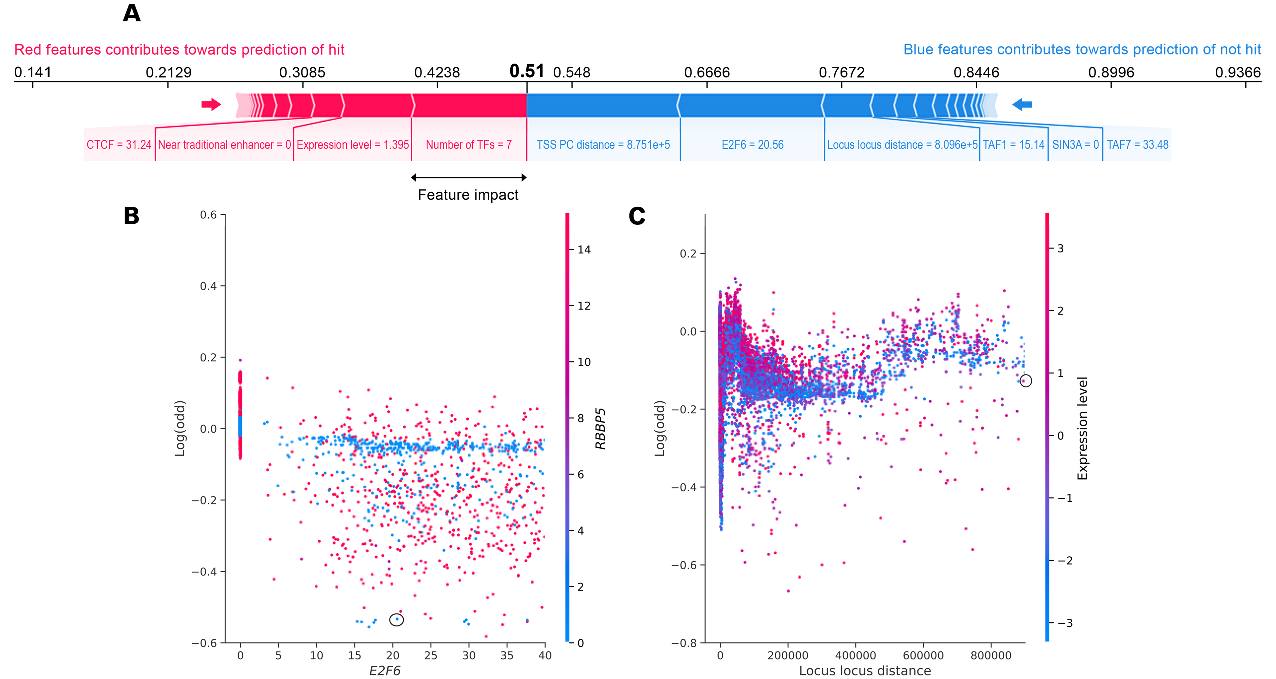
\includegraphics[scale=0.6]{plots/results/ml/model.exp.linc00798.pdf}
  \caption[Model explainability for \textit{LINC00879}]{\textbf{Model explainability for \textit{LINC00879}}. \textbf{(A)} Explained hit probability for \textit{LINC00879}. \textbf{(B)} SHAP dependence plots for \textit{E2F6}, and \textbf{(C)} lncRNA-PC distance distance versus their SHAP values. Circles highlight \textit{LINC00879}.}
  \label{fig:model-exp-lnc}
\end{figure}

The mild increased in hit probability shown in \autoref{fig:model-exp-lnc}A was driven mainly by 4 features: \textbf{1)} "\textit{number of TFs}", \textbf{2)} "\textit{expression level}", \textbf{3)} "\textit{distance from a traditional enhancer}", and \textbf{4)} \textit{CTCF}. The risk explanation bar in \autoref{fig:model-exp-lnc}A has red features that push the hit probabilities higher (to the right) and blue features that push the probabilities lower (to the left). Each group of features is sorted by the magnitude of their impact and the features with the greatest impact were labelled. Through this representation, we found that many of the 71 features had a small impact on \textit{LINC00879} case and the hit probabilities for \textit{LINC00879} were predominantly driven by 10 features. 

The reason \textit{LINC00879} obtained a 0.51 hit probability was mainly for being isolated from PCGs, the closest one being \textit{NSUN3}. This explains "\textit{TSS-PC}" and "\textit{lncRNA-PC distance}" features. Notably, transcription factors \textit{E2F6}, \textit{TAF1}, and \textit{TAF7} showed a negative effect. Next, to understand the role of these TFs SHAP dependence plots reported a correlation between \textit{E2F6} and \textit{RBBP5} (\autoref{fig:model-exp-lnc}B) , and "\textit{locus-locus distance}" and "\textit{expression}" (\autoref{fig:model-exp-lnc}C). For "\textit{locus-locus distance}" and "\textit{transcript expression}" two clusters were reveleaded, if "\textit{locus-locus distance}" increased on average the hit probability decreased unless transcripts presented an expression level > 0 FPKMs. For \textit{E2F6} and \textit{RBBP5} the clustering was less clear.  

\subsection{Further experimental validations to uncover cell-growth related lncRNAs}
\label{sec:list-lncRNA-validate}

The lncRNA \textit{LINC00879} was one example where our XGBoost model predicts a lncRNA transcript to be functional and the CRISRPRi library\autocite{liu_2017_crispri} labelled as not functional (false positive case). After thoughtful inspection of false positive transcripts in K562 cell, we selected a list of 40 transcripts to experimentally validate them (\autoref{tab:lncRNA-validate}), as we already validated \textit{LINC00879}.

Our aim is to uncover the maximum number of functional lncRNAs related to cell-growth, in the most efficient way, thus while we validate our candidate genes we could re-train our model. Following this approach, we could further understand the most important features that affect cell-growth and improve sensitivity and specificity values of our model. 

\begin{table}[!htb]
  \caption[List of 40 lncRNAs for experimental validation]{\textbf{List of 40 lncRNAs for experimental validation}}
  \begin{scriptsize}
    \begin{tabulary}{0.95\linewidth}{cccccc}
      \textit{AC005307} & \textit{AC005381} & \textit{AC010601} & \textit{AC012615} & \textit{AC074050} & \textit{AC096559} \\
      \textit{AC097532} & \textit{AC246817} & \textit{AL034397} & \textit{AL035446} & \textit{AL158066} & \textit{AL162413} \\
      \textit{AL691447} & \textit{AP000855}  & \textit{AP006222} & \textit{CUFF5183312} & \textit{FAM157C} & \textit{FAM41C} \\
      \textit{LINC00221} & \textit{LINC00680} & \textit{LINC00861} & \textit{LINC00879} & \textit{LINC01029} & \textit{LINC01203} \\
      \textit{LINC01410} & \textit{LINC01420} & \textit{LINC01608} & \textit{LINC02062} & \textit{LINC02154} & \textit{LINC02432} \\
      \textit{MINCR} & \textit{MIR4435-2HG} & \textit{NUTM2A-AS1} & \textit{NUTM2B-AS1} & \textit{PDXDC2P} & \textit{RP11-706O15} \\
      \textit{RP11-94P11} & \textit{SNHG1} & \textit{SNHG6} & \textit{ZFHX4-AS1} \\
    \end{tabulary}
  \end{scriptsize}
  \label{tab:lncRNA-validate}
\end{table}

\clearpage

\subsection{Discussion: XGBoost classifier to uncover the function of lncRNAs in cell-growth}
\label{sec:ml-discussion}

CRISPRi (CRISPR interference) is an established genome-wide technology to knockdown lncRNA transcripts in diverse cellular contexts. While the idea to inhibit lncRNA transcription in a high-throughput level is not novel,\autocite{liu_2020_crispri,Haswell_2021_crispri} the present work brings novelty in the field by combining: \textbf{1)} the supervised extreme gradient boosting (XGBoost) algorithm, \textbf{2)} transcription factor (TF) ChIP-seq data, and \textbf{3)} high-throughput screens to uncover the function of lncRNAs in the following human cell lines: iPSC, K562, U87, MCF7, MDA-MB-231, HeLa, and HEK293T. 

More importantly, our work added value by unveiling the cell-growth role of \textit{LINC00879} in the K562 cell line, with the aid of our cost-sensitive XGBoost classifier trained with Liu \textit{et al.} CRISPRi and ENCODE TF ChIP-seq datasets.\autocite{liu_2020_crispri,encode_2011_user,encode_2004} We were able to quantify the advantage of adding TF narrow-peaks around lncRNA core promoters, using XGBoost, and recursively eliminate non-contributing features based on Shapley values. We obtained a performance of mean AUROC of 0.8250 with our approach, which overperformed when compared to previous results (mean AUROC of 0.753\autocite{liu_2020_crispri}). Additionally, we obtained balanced sensitivity and specificity values (0.8227 and 0.7292, respectively) across all seven studied cells, even with a clearly under-representation of hits compared to not hits (on the order of 1:55). As a result of our satisfactory hit-classifier performance plus an association of the previously unknown \textit{LINC00879} with K562 cell-growth rate; 40 lncRNA genes with unknown function were selected as candidates for experimental validation in the K562 cell type. 

By obtaining the local and global explanations of our trained classifier with the 71 selected features (16 from the CRISPRi screening, and 55 from ENCODE TFs) based on Shapley values, our study showed that "\textit{distance between lncRNA-TSS and its nearby coding gene}", "\textit{expression level}", and "\textit{number of TFs with ChIP-seq signal}" features were the top 3 most important for our tree-based model. The feature "\textit{number of TFs}", to the best of our knowledge, is the first time that is highlighted to be relevant, using ML algorithms. In contrast, the importance of "\textit{expression level}" to link functionality to a noncoding locus, is a well-recognized result.\autocite{liu_2020_crispri,Haswell_2021_crispri} Moreover, Shapley values suggested that some genomic features, that globally may not be relevant, may actually be important for some specific transcripts. This suggests that lncRNAs involved in cell-growth follow a non-linear relationship with the described features, implying the necessity for functional screenings.

Nonetheless, CRISPRi  screens display non-negligible off-target effects. Additionally, a number of publications have reported that reverse-genetics assays show discrepancies among the cellular phenotypes and the number of differentiated genes obtained with different inhibition methods.\autocite{stojic_2018_specificity} More importantly, a very large gap exists between reporting biological function of lncRNAs in cell lines and the difficulty in obtaining such evidence in \textit{in-vivo} studies; this is true even for the lncRNAs considered as "\textit{gold standard}", such as \textit{Malat1}, \textit{Neat1}, etc.\autocite{gao_2020_reverse_genetics}  We obtained increased power to discriminate between hits and not hits by adding TF ChIP-seq data. This indicates that there is still room for improvement. For instance, conservation information (\textit{e.g.} sequence-conservation of promoters, transcripts and exon transcripts; plus synteny data) should be incorporated to understand how this feature plays a role to uncover noncoding transcripts involved in cell-growth; and adding more biological interpretability. Further, as distance between lncRNA TSS and its nearby protein-coding gene was ranked as the most important feature for our work, a more comprehensive lncRNA genomic-classification (\textit{i.e.} divergent lincRNA, convergent lincRNA, nested genic-exonic or intronic, etc.) should be included. Additionally, including splicing efficiency across ENCODE cell lines could be beneficial for our mode, as it has been for Haswell \textit{et al.}\autocite{Haswell_2021_crispri} Moreover, as the \textit{LINC00879 UCSC} plot reported, ENCODE epigenetic features should also be incorporated.  

In future implementations, our work could benefit from new available functional screenings based on CRISPRi and individual experimental validations from lncRNA candidate genes to re-train our model (\textit{e.g.} the results of our 40 lncRNA candidates); achieving a dynamic process. For instance, the new available CRISPRi library produced from Haswell \textit{et al.}\autocite{Haswell_2021_crispri} could be used as a validation-set for a robustness assessment of our algorithm; in addition to increasing the lncRNA hit percentage. This dynamic process could lead to the development of a web interface available to the community to serve as a predictive-tool to uncover functional lncRNAs in the context of cell-growth, and eventually other phenotypes, in human cell lines. All our analyses were based on supervised ML methods. However, we could harness the  weakly-unsupervised and the unsupervised strategies to allow the ML models to learn from the data itself. One analysis that can be performed is using the entire highly dimensional dataset and performing a k-means clustering; collapsing the data into two dimensions. Subsequently, visualizing the results through a t-SNE or UMAP plot. What we would expect to see is two different clusters, hits and not hits, nonetheless this result is unlikely because hit and not hits share a lot of common features, the latter result was observed by.\autocite{Haswell_2021_crispri}

At the early stage of our study, we tried to use the data from the \textit{LnCompare} database,\autocite{carlevaro_2019_lncompare} which contains interesting features full of biological richness, such as subcellular localization, expression across human tissues, tissue specificity (using the $\tau$ metric), etc. Nevertheless, the information is at the gene level instead of the transcript level, consequently we could not use that dataset. So collaborating with the \textit{LnCompare} developers to achieve transcript level data could be relevant for this project and for the lncRNA field.  

\clearpage

\section[LncRNA analysis of the \textit{Drosophila} genome during regeneration]{LncRNA analysis of the \textit{Drosophila} genome during regeneration}
\label{sec:results-dme}

\subsection{Characterization of cell-damage lncRNAs}
\label{sec:ge-reg-results}

To elucidate the role of lncRNAs within the \textit{Drosophila melanogaster} genome after cell-death induction, Vizcaya-Molina \textit{et al.}\autocite{vizcaya_2018} data was analyzed, using three time points after cell-damage: early (0h), mid (15), and late (25h). QC results demonstrated problems with replicate: \textit{control-0h-r2}, with a variability > 3 standard deviations from the rest of replicates (\autoref{supp-fig:connectivity-reg}) . In consequence, replicate \textit{control-0h-r2} was removed.

131 differentially expressed (DE) lncRNAs were identified. DE results revealed the early time point with the highest number of upregulated lncRNAs (\autoref{fig:dge-pc-lncRNA}A). Interestingly, downregulated lncRNAs at 15h obtained the highest number of DEGs, with 56 cases (see \autoref{tab:deg_complete}). As expected, lncRNAs demonstrated a time point specific expression, with 4 and 7 DEGs in all time points (\autoref{fig:dge-pc-lncRNA}B). 

\begin{figure}[!htb]
  \centering
  \includegraphics[scale=0.33]{plots/results/dme/PC.lncRNA.results.pdf}
  \caption[DE genes after cell-death induction]{\textbf{DE genes after cell-death induction}. \textbf{(A)} Number of lncRNA and PC DEGs. \textbf{(B)} LncRNA venn diagrams in early, mid, and late time-points. \textbf{(C)} PCG venn diagrams.}
  \label{fig:dge-pc-lncRNA}
\end{figure}

For PCGs, 1,627 DE genes were identified among them the \textit{reaper} (\textit{rpr}) and the \textit{Growth arrest and DNA damage-inducible 45} (\textit{Gadd45}) genes were found upregulated at 0h. \textit{Gadd45} is known to be required in response to stress, apoptosis, and proper regeneration of wing imaginal discs,\autocite{camilleri_2019,blanco_2010} and \textit{rpr} was the gene used to induce cell-damage.\autocite{vizcaya_2018} PCGs compared with lncRNAs showed a higher overlap of DEGs in the three time points (\autoref{fig:dge-pc-lncRNA}C).

LncRNA time-point and regeneration-specificity results revealed the early time-point with the highest number of genes experimenting with a time-point-specific expression with 14 and 8 genes expressed only at 0h or at 0h and 15h, respectively (\autoref{fig:time-point-reg-specific}A).  Same pattern was observed for regeneration specific expression (\autoref{fig:time-point-reg-specific}B). Increased time-point specificity at the early time point was preserved by dividing the genes by their DE status (\autoref{fig:time-point-specific-up-down}). 

\begin{figure}[ht!]
  \centering
  \includegraphics[scale=0.6]{plots/results/dme/time.point.reg.specificity.pdf}
  \caption[Time-point and regeneration-specificity results]{\textbf{Time-point and regeneration-specificity results}. \textbf{(A)} Time-point specificity analysis of the 131 DE lncRNAs. Time Point (TP) specific= lncRNA expressed only on the analyzed time-point. \textbf{(B)} Regeneration analysis of lncRNAs upregulated. Reg specific= not expressed in control.}
  \label{fig:time-point-reg-specific}
\end{figure}

We explored the DE status of the 131 DE lncRNAs across regeneration; identifying that 4 up and 7 down genes were DE in all time points, and that the vast majority of upregulated and downregulated genes were DE at the early time point and then not differentially expressed (NDE) in other time points (\autoref{fig:chracterization-lncRNAs}A). For lncRNAs NDE at 0h the majority were downregulated at 15h and then NDE at 25h. Two hairpin genes and \textit{CR40469} were the top 3 most expressed genes that were upregulated at 0h. Moreover, \textit{CR34335} and \textit{rox2} were the most expressed downregulated genes at 0h. To evaluate whether our differentially expressed lncRNAs were indeed not coding, coding potential assessment tool (CPAT) was used to score for coding potential.\autocite{wang_2013_cpat} Comparing the CPAT score of our DE lncRNAs to FlyBase annotated lncRNAs and PCGs expressed indicated that our DE lncRNAs reported a very low coding potential (\autoref{fig:chracterization-lncRNAs}B). None of our genes exceeded the threshold of 0.39, calibrated for discriminating coding from noncoding genes in \textit{Drosophila melanogaster} (\textit{D. melanogaster}).\autocite{wang_2013_cpat}

The 2,455 lncRNAs annotated within \textit{D. melanogaster} were dispersed throughout the genome, including intergenic (56.54\%), genic intronic (17.11\%) or genic exonic (26.35\%), with respect to neighboring PCGs (\autoref{fig:gw_lncRNA_class}).  In our DE set, intergenic was the most frequent class for early up with 44.83\% and for ealry down with 57.58\% (\autoref{fig:chracterization-lncRNAs}C); genome-wide intergenic lncRNAs were also the most common class. Interestingly, for upregulated genes at 15h genic intronic was the most frequent group (\autoref{supp-fig:mid-late-class}A; \textit{p-value}= 1.17e$^{-4}$; \textit{two-sided Fisher exact test}). On average, the percentage of overlapping between DE genic-exonic and their PCGs was 27.9\%, which was significantly lower than the rest of annotated genic-exonic genes (\textit{Wilcoxon test}, \textit{p-value}= 2.08e$^{-6}$).

\begin{figure}[ht!]
  \centering
  \includegraphics[scale=0.37]{plots/results/dme/chr.lncRNA.early.v2.pdf}
  \caption[LncRNA patterns after cell-damage]{\textbf{LncRNA patterns after cell-damage}. \textbf{(A)} Behavior of the 131 DE lncRNAs across regeneration. \textbf{(B)} Coding potential of the 131 DE lncRNAs, all annotated lncRNAs, and PCGs. \textbf{(C)} LncRNA classification of early DE lncRNAs. }
  \label{fig:chracterization-lncRNAs}
\end{figure}

Subclassification of lncRNAs highlighted divergent lincRNAs (long intervening noncoding RNAs) and intronic nested genes as the most representative subgroups of intergenic and intronic classes, respectively (\autoref{tab:lncRNAs-subclass}). Distance analysis between lncRNA TSS and PCG demonstrated that our DE subgroup of divergent lincRNAs (2,499 bp) presented a significantly lower distance compared to genome-wide divergent lincRNAs (4,153 bp; \textit{Wilcoxon test}, \textit{p-value}= 0.012), which may reflect a biological importance to be near from a PCG. Further, ATAC-seq results consistently with gene expression and DE analyses, indicated that in the early stage the TSS of upregulated lncRNAs were more accessible in regeneration compared to downregulated, and NDE lncRNA genes (\autoref{fig:atac-seq}). 

\begin{figure}[ht!]
  \centering
  \includegraphics[scale=0.7]{plots/results/dme/atac.seq.agg.early.pdf}
  \caption[ATAC-seq profiles for DE and NDE lncRNAs at the early time point]{\textbf{ATAC-seq profiles for DE and NDE lncRNAs at the early time point}. Aggregation plots around the TSS of up, down, and NDE lncRNAs ($\pm$400 bp) at the early stage of cell-death induction (0h). NDE= not differentially expressed lncRNAs.}
  \label{fig:atac-seq}
\end{figure}

\subsubsection{PCGs associated to the DE lncRNAs are enriched in cell-death and developmental terms}
\label{sec:go-lncRNAs}

Gene ontology (GO) enrichment of neighboring and overlapping PCGs (see \nameref{sec:gene_ontology_enrichment}) was used to assess the potential biological function of lncRNA genes within regeneration. After correction for multiple testing, overlapping PCGs showed significant GO terms for: programmed cell death, regulation of cell cycle and development (\autoref{fig:go_genic_intergenic}A). Subsequently, we combined neighboring and overlapping PCGs identifying more biological terms, such as: wing imaginal disc morphogenesis and development, \textit{Jak-STAT} cascade, and developmental processes (\autoref{fig:go_genic_intergenic}B). The \textit{Jak-STAT} pathway is required for regenerative growth and interestingly is not likely to occur in development, which may indicate that PCGs associated with the DE lncRNAs are involved in regeneration pathways and wound healing processes.\autocite{katsuyama_2015,santabarbara_2015}

\begin{figure}[ht!]
  \centering
  \includegraphics[scale=0.65]{plots/results/dme/go.genic.intergenic.pdf}
  \caption[GO terms of PCGs associated with the DE lncRNAs]{\textbf{GO terms of PCGs associated with the DE lncRNAs}. \textbf{(A)} GO of PCGs which overlapped a genic DEG. \textbf{(B)} GO based on the combination of PCGs which overlapped a genic DEG, and the two closer PCGs (up and down stream) from a lincRNA DEG. Size of circles denote number of genes of each term.}
  \label{fig:go_genic_intergenic}
\end{figure}

\subsubsection{Relationships between lncRNAs and nearby PCGs}
\label{sec:lncRNA-PC-correlation}

The relationship between lncRNAs and their neighboring PCGs during regeneration was assessed by following two approaches. First, by analyzing the DE status of each gene type (\nameref{paragraph:de-status}). Second, by classifying their expression pattern during wound healing (\nameref{paragraph:expression-classification}).

Each lncRNA was assigned to its overlapping or closest PGC (see \nameref{sec:lncRNA_pc_co-expression}), forming lncRNA-PCG pairs that were used to evaluate their association. We obtained 134 pairs for lincRNA-PCG, with a maximum of 1 lincRNA (\textit{CR42868}) neighboring 10 PCGs. On average, the divergent-lincRNA class was the closest subgroup to their neighboring PCGs (\autoref{supp-fig:lincRNA-distance}). Subsequently, we combined the 134 lincRNA-PCG pairs with 76 genic-PCG pairs obtaining a total of 210 lncRNA-PCG pairs. We allowed multiple-overlaps for genic lncRNAs; the genic-exonic \textit{CR45600} overlapped with 3 PCGs, which was the locus with the highest overlap number.

\paragraph{The DE status of lncRNA-PCG pairs reveal low relationship}
\label{paragraph:de-status}

Investigation of the DE status of lncRNA-PCG pairs demonstrated a low relationship between them. On average, 90\% of PCGs were flat while the lncRNAs were DE. At the early time point in regeneration, and at the mid time point in control were the highest and lowest percentages of relationship, respectively (\autoref{fig:co-exp-cat-2}A,B). Interestingly, \autoref{fig:co-exp-cat-2} reported more concordant cases in all our studied conditions.

\begin{figure}[ht!]
  \centering
  \includegraphics[scale=0.55]{plots/results/dme/co.expression.cat.pdf}
  \caption[DE status of PCGs nearby DE lncRNAs]{\textbf{DE status of PCGs nearby DE lncRNAs}. \textbf{(A,B)} In regeneration or in control, respectively.}
  \label{fig:co-exp-cat-2}
\end{figure}

At the early time point, 16\% relationship represented 8 concordant cases (5 genic-exonic, 2 genic-intronic and 1 intergenic) and 1 discordant case (1 intergenic). Additionally, 44\% of neighboring PCGs were uncharacterized, and characterized PCGs were involved in metabolic processes.

\begin{figure}[ht!]
  \centering
  \includegraphics[width=1\textwidth]{plots/appendix/dme/cr43611.ucsc.plot.pdf}
  \caption[\textit{CR43611 UCSC} plot]{\textbf{\textit{CR43611 UCSC} plot}. RNA-seq data, gene structure, conservation, and repeats of \textit{CR43611} lncRNA. Blue boxes represent coding and noncoding genes. .}
  \label{fig:cr43611-ucsc}
\end{figure}

An interesting concordant case was the \textit{CR3611}-\textit{chaski} (\textit{chk}) pair (genic-intronic and PCG, respectively) which both were upregulated at all time points (\autoref{fig:cr43611-ucsc}). The \textit{chk} gene has been observed to be involved under stress conditions in glial cells.\autocite{delgado_2018} For the discordant case, the intergenic \textit{CR44899} was only upregulated at the early time point and its neighboring PCG \textit{CG13258} was downregulated at the three time points (\autoref{supp-fig:cr43611-ucsc}). To the best of our knowledge, the role of \textit{CG13258} is unknown. These analyses allowed us to establish a relationship between \textit{CR3611} and \textit{CR44899} lncRNAs and their neighboring PCGs ("\textit{guilt-by-association}" \textit{in-cis}\autocite{signal_2016_computational}), although more analyses are needed to confirm their relationship. 

\paragraph{Classification of lncRNA-PCG expression show higher relationship}
\label{paragraph:expression-classification}

Using our expression classification approach (see \nameref{sec:lncRNA_pc_co-expression}) resulted in 33\% more lncRNA PCG relationships compared to observing the DE status of lncRNA PCG pairs. Focusing on regeneration, we identified that most of the DE lncRNAs were labeled as decreasing, followed by valley, peak and increasing classification (\autoref{fig:co-exp}A), in contrast peak and valley were the top 2 more common classes in control (\autoref{supp-fig:co-exp-ctrl}A).  

\begin{figure}[ht!]
  \centering
  \includegraphics[scale=0.6]{plots/results/dme/co.expression.results.pdf}
  \caption[Co-expression results]{\textbf{Co-expression results}. \textbf{(A)} Co-expression classification in regeneration. \textbf{(B)} Co-expression results in regeneration. \textbf{(C)} Summarization of different co-expression associations in control and in regeneration.}
  \label{fig:co-exp}
\end{figure}

On average, we identified 44\% of gene expression association between lncRNA-PCG pairs. As well as with our previous analysis, we found more concordant cases (36 cases for control and regeneration conditions; \autoref{fig:co-exp}B and \autoref{supp-fig:co-exp-ctrl}B). We observed a higher number of lncRNA-PCG associations using this approach compared to the former approach (observing the DE status of lncRNA-PCG pairs), the reason is this approach is less restrictive. 

Interestingly, by focusing in regeneration and by their genomic position, the relationship frequencies order changed, for genic-intronic the most common case was concordant instead of no association, suggesting a higher probability of \textit{cis-acting}  mechanism between genic intronic and their overlapping PCGs\autocite{perez_blister, pelechano_2013} (see \autoref{fig:co-exp-supp-fig}A). Peak and valley were the most common classes for concordant and discordant scenarios, respectively (\autoref{fig:co-exp-supp-fig}B). Combining regeneration and control relationship results demonstrated as expected no-association between lncRNA-PCG pairs as the most common case (\autoref{fig:co-exp}C). Additionally, a higher association in control compared to regeneration was reported. However, we were more interested in cases where we observed positive and negative associations both in control and in regeneration (\autoref{fig:co-exp}C). Hence, we thoroughly examined 15 and 10 positive and negative associations, respectively.

\begin{figure}[ht!]
  \centering
  \includegraphics[scale=0.6]{plots/results/dme/co.expression.examples.pdf}
  \caption[\textit{CR40469} and \textit{CR43956} co-expression]{\textbf{\textit{CR40469} and \textit{CR43956} co-expression}. \textbf{(A)} Concordant in control and discordant in regeneration. \textbf{(B)} Concordant in control and in regeneration. Expression= log$_{10}$(TPM+0.1).}
  \label{fig:co-exp-examples}
\end{figure}

\textit{CR40469}-\textit{RhoGAP1A} and \textit{CR43956}-\textit{anne} pairs were two examples of a positive-negative and a positive-positive association in control and in regeneration, respectively. The lincRNA \textit{CR40469} has a distance of 4.7 Kb from its neighbor PCG \textit{RhoGAP1A}, \textit{CR40469} was upregulated at 0h and 25h, and \textit{RhoGAP1A} was expressed but NDE in all time points. In control, the  \textit{CR40469}-\textit{RhoGAP1A} pair displayed the same expression pattern, with higher expression at the mid time point. By contrast, during regeneration \textit{CR40469} changed its expression from peak to valley (opposite expression pattern); and \textit{RhoGAP1A} maintained the same expression pattern (\autoref{fig:co-exp-examples}A). These results suggest a relationship between \textit{CR40469} and \textit{RhoGAP1A}, thus are an interesting pair to experimentally validate this initial hypothesis. 

The genic-intronic \textit{CR43956} overlaps in antisense with the PCG \textit{anne}, \textit{CR43956} was downregulated at 15h, and \textit{anne} was downregulated at 25h. The \textit{CR43956}-\textit{anne} pair demonstrated the same pattern of expression both in control and in regeneration (\autoref{fig:co-exp-examples}B). In consequence, there could be other interesting pairs to further analyze. 


\subsubsection{Functional and non-functional genomic features for our DE lncRNAs}
\label{sec:genomic-features}

DE lncRNAs presented an over-representation of genes with multiexons on their longest transcript compared to NDE (\textit{Fisher exact test}, \textit{p-value}= 0.0104; \autoref{supp-fig:number-exons}). According to Liu \textit{et al.} logistic regression model,\autocite{liu_2017_crispri} number of exons is a mild feature for lncRNA functionality (odds= 1.1 and \textit{p-value}= 5.74e$^{-3}$). Additionally, lncRNAs with multiple isoforms were more present in DE lncRNAs, compared to NDE (\textit{Fisher exact test}, \textit{p-value}= 4.36e$^{-5}$; \autoref{supp-fig:isoform-analysis}). 

Overall, lncRNA exons showed a lower GC content compared to PCG exons (\textit{Wilcoxon test}, \textit{p-value}= 1.56e$^{-7}$) as observed by.\autocite{lopez_2017} In addition, analyzing GC\% of promoters, genes, and the longest transcript from DE and NDE lncRNAs, significant lower GC content was observed with 0.0185, 1.09e$^{-6}$, and 2.44e$^{-5}$ adjusted \textit{p-values}, respectively (\textit{Wilcoxon test}; \autoref{supp-fig:gc-content}). Next to better understand GC content results, analyses based on lncRNA classification, and comparing DE to lncRNA expressed and not expressed (NE) were performed. We Iidentified significant differences among intergenic lncRNAs, with 0.01 and 6.01e$^{-4}$ adjusted \textit{p-values}, respectively (\textit{Wilcoxon test}; \autoref{fig:genomic-cha}A). High GC content has been observed in functional lncRNAs with more stable secondary structures,\autocite{lopez_2017} however GC\% is not the most determinant feature to assign functionality to lncRNAs.\autocite{haswell_2020}

Finally, length analyses based on the longest transcript reported a lower length contrasting DE genic intronic to NDE genic intronic (\textit{Wilcoxon test}, adjusted \textit{p-value}= 0.031; \autoref{fig:genomic-cha}B). 

\begin{figure}[ht!]
  \centering
  \includegraphics[scale=0.6]{plots/results/dme/gc.length.pdf}
  \caption[Genomic features of our lncRNA DE list]{\textbf{Genomic features of our lncRNA DE list}. \textbf{(A)} GC\% between DE, expressed, and NE. \textbf{(B)} Length analysis based on the longest transcript, \textit{y-axis} in log$_{10}$(bp). Expressed= lncRNA expressed in control or/and regeneration, NE= not expressed, and n.s.= not significant.}
  \label{fig:genomic-cha}
\end{figure}

\subsubsection{Low sequence-conservation for our DE lncRNAs in 27 insect species}
\label{sec:sequence-conservation}

Sequence-conservation was defined as homology higher than 0.25 in at least \textit{D.melanogaster} and other insect species (\autoref{fig:seq-conser-early}C).  Conservation analyses were performed at two levels: gene, and transcript with 35.88\%, and 59.54\% of lncRNAs conserved from the 131 group of DE genes, respectively. As expected, at transcript level lncRNAs were more conserved compared to gene level, where lncRNA introns are less conserved.\autocite{lopez_2017,nitsche_2017,ulitsky_2016_evolution}

No statistical difference was observed between DE and NDE genes. Moreover, by their location classification, the lincRNA (lincRNA and intergenic terms were used indistinctly) group was the most conserved at gene and transcript level, with 24 and 39 conserved lincRNAs, respectively. To observe in more detail the conservation of lncRNAs within their time point and DE status, we plotted each conserved lncRNA by early (\autoref{fig:seq-conser-early}A), mid (\autoref{supp-fig:lncRNA-seq-conservation}A), and late (\autoref{supp-fig:lncRNA-seq-conservation}B) time points.

At the early time point, 38.71\% and 61.29\% were conserved at gene and transcript level, respectively; from which 11 exonic, 6 intronic and 21 intergenic were conserved at the transcript level (\autoref{fig:seq-conser-early}A). \textit{CR45182} (4 species, 0.833 homology, and downregulated), \textit{CR44993} (24 species, 0.698 homology, and upregulated), and \textit{CR45433} (3 species, 1 homology, and upregulated) were the most conserved by exonic, intronic, and intergenic classification, respectively. Highlighting by DE status and lncRNA classification, genic-exonic up (58.33\%) and intergenic down (78.95\%) were the most conserved subgroups (\autoref{fig:seq-conser-early}B). Unclear sequence conservation clustering was observed between up and down genes, except for genic-intronic at the late time point (\autoref{supp-fig:lncRNA-seq-conservation}B).

\begin{figure}[ht!]
  \centering
  \includegraphics[scale=0.75]{plots/results/dme/seq.by.exon.pdf}
  \caption[Sequence-conservation of early DE lncRNAs at the transcript level]{\textbf{Sequence-conservation of early DE lncRNAs at the transcript level}. \textbf{(A)} Dots represent a lncRNA, and \textit{y-axis} reports the number of species that present the lncRNA conserved. \textbf{(B)}. Conserved and not conserved genes by DE status, and classification. \textbf{(C)} Phylogenetic tree with the 27 insect species used for the conservation analysis.}
  \label{fig:seq-conser-early}
\end{figure}

\clearpage

\subsection{LncRNA developmental and tissue signatures}
\label{sec:dme-results-second-part}

From the 131 DE lncRNAs in regeneration, we explored their general expression properties through development, using \textit{D. melanogaster} embryonic, larval, and pupal developmental stages obtained from the modENCODE project\autocite{celniker_2009,modencode_2010} (\autoref{fig:t-sne-mode-encode}A). Five well-known developmental PCGs were analyzed to assess a correct developmental pattern.\autocite{batut_2017} \autoref{supp-fig:markers-dev} confirmed an expected behavior from these five genes across embryonic development. The developmental markers \textit{Pgc}, \textit{Prd}, \textit{Gsb}, \textit{Mas} and \textit{Edg78E} showed an expression peak at 0-2h, 2-4h, 4-6h, 12-14h, and 18-20h, respectively. The same developmental oscillation was observed by Batut \textit{et al.}\autocite{batut_2017} In consequence, these results confirm the quality of the analyses and the developmental data.

\begin{figure}[ht!]
  \centering
  \includegraphics[scale=0.6]{plots/results/dme/modencode.fist.fig.pdf}
  \caption[t-SNE of developmental samples]{\textbf{t-SNE of developmental samples}. \textbf{(A)} Developmental time points analyzed. \textbf{(B)} t-SNE based on expressed genes, coding and noncoding, in log$_{10}$(TPM+0.1) within the developmental dataset.}
  \label{fig:t-sne-mode-encode}
\end{figure}

t-SNE based on expressed PCGs and lncRNAs revealed a clear cluster separation between embryonic and larval stages relative to pupal stages (\autoref{fig:t-sne-mode-encode}B), the same results were observed using a PCA (\autoref{supp-fig:pca-modencode}). Additionally, a timeline pattern and clustering among replicates were reported. 

Most of our DE lncRNAs in regeneration at the early time point showed dynamic expression patterns across development (\autoref{fig:heatmap-mod-dev}), 17.24\% and 24.24\% of lncRNAs upregulated and downregulated in regeneration, respectively were not expressed in the developmental time points used in our analysis. Hierarchical clustering of lncRNAs upregulated at the early time point highlighted 3 main clusters. In the first lncRNA cluster, genes were mainly expressed during embryonic time points (0h-24h). In the second cluster, genes were developmental-specific. Finally, the third cluster which represented the 8.3\% of lncRNAs, genes were highly expressed in all developmental time points (\autoref{fig:heatmap-mod-dev})

\begin{figure}[ht!]
  \centering
  \includegraphics[scale=0.6]{plots/results/dme/two.heatmaps.modencode.pdf}
  \caption[DE lncRNAs expressed through development]{\textbf{DE lncRNAs in cell-death conditions expressed through \textit{D. melanogaster} development}. Heatmaps based on gene expression (log$_{10}$ transformation plus 0.1 as a pseudo-count) of lncRNAs up and downregulated in regeneration (left and right plot, respectively). Developmental samples were collapsed by their mean expression and ascendingly sorted.}
  \label{fig:heatmap-mod-dev}
\end{figure}

Interestingly, the top 2 most expressed DE lncRNAs in regeneration were: \textit{hpRNA:CR33940} and \textit{hpRNA:CR32207}, which were also the top 2 most expressed in development from the 131 DE group. Similarly, \textit{CR34335}, \textit{rox2}, and \textit{CR43264} downregulated lncRNAs in regeneration were also the top 3 most expressed across development from the DE group. High gene expression of \textit{hpRNA:CR32207}, \textit{hpRNA:CR33940}, and \textit{rox2} within the regeneration and the developmental datasets can be linked to their stem-loop structure. LncRNA hairpin structures are linked to post-translational modifications and elevated gene expression,\autocite{statello_2021_lncRNA_reg} and lncRNA \textit{rox2} is part of the male-specific lethal complex (MSL) which is a key player in fruit fly dosage compensation.\autocite{flintoft_2013_rox,ilik_2013_rox} Single-cell analyses from Davie \textit{et al.} in \textit{Drosophila} brain highlight the lncRNA \textit{CR34335} as the few genes with no signals of decline with age and high mean expression,\autocite{davie_2018} these results are in agreement with our observations. 

Summarizing the three time-points analyzed in regeneration (early, mid and late), 24.76\% from the 131 DE lncRNAs were not expressed in the selected developmental samples, and 78\% of the DE genes in regeneration demonstrated condition-specific expression patterns. At the genome-wide level, 55.32\% of annotated lncRNAs were not expressed in any analyzed developmental stage, with the exception of 4\% of lncRNAs and the pupal stage, lncRNA presented condition-specific expression patterns (\autoref{fig:heatmap-modencode-dev-all}). Higher expression for lncRNAs in the pupal stage compared to embryonic and larval stages was also observed by.\autocite{chen_2016_lncRNA}

\subsubsection{DE lncRNAs present dynamic expression across development}
\label{paragraph:modENCODE-clusters}

K-means clustering was applied to more formally assess the dynamic expression of the DE lncRNAs in regeneration during development. According to the results from \autoref{fig:t-sne-mode-encode}B and \autoref{supp-fig:pca-modencode}, the clustering-analysis was applied dividing the developmental dataset in two groups: \textbf{1)} the embryo-larvae group and  \textbf{2)} the pupae group.

\begin{figure}[ht!]
  \centering
  \includegraphics[scale=0.6]{plots/results/dme/embryo.clusters.pdf}
  \caption[Six embryonic and pupal developmental clusters]{\textbf{Six embryonic and pupal developmental clusters}. K-means clustering based on embryonic and pupal gene-expression (blue and brown lines, respectively). \textit{Y-axis} shows the normalized and scaled gene-expression levels. \textit{X-axis} denotes the developmental time-points ascendingly sorted. Left-numbers show the number of the 131 DE lncRNAs contained in each developmental cluster.}
  \label{fig:k-means}
\end{figure}

Six clusters were obtained from the embryo-larvae group, containing 30 of the 131 DE lncRNA genes, with highly correlated expression during development (\autoref{fig:k-means}; mean \textit{Pearson's correlation}= 0.87). All embryonic-larval clusters contained lncRNAs DE in regeneration, the frequency of the DE lncRNAs within the clusters was balanced, although cluster 3 and cluster 5 contained the highest number of the DE lncRNAs with 6 genes in both clusters. Cluster 3 contained lncRNAs lowly expressed across all time points, and cluster 5 contained genes with a decreased expression trend and after embryo 22-24h an increase was observed. 

The larvae-group revealed nine robust-clusters, containing 49 of the 131 DE lncRNA genes, from which clusters 4, 5, 7, 8, and 9 (\autoref{fig:k-means-pupae}) presented more dynamics compared to clusters 1, 2, 3, and 6 (\autoref{supp-fig:pupae-clustering}), which were clustered for their expression level. The nine pupal-clusters contained at least one DE lncRNA; cluster 2 and cluster 4 contained the highest number of DE lncRNAs, with 14 and 8, respectively. In cluster 2, lncRNAs presented a mild decrease of expression during pupal development, and cluster 4 contained genes that decreased their expression from pupae 24h. 

\begin{figure}[ht!]
  \centering
  \includegraphics[scale=0.6]{plots/results/dme/pupae.clusters.pdf}
  \caption[Pupal developmental clusters]{\textbf{Pupal developmental clusters}. K-means clustering based on pupal developmental expression (green line). \textit{Y-axis} shows the normalized and scaled gene expression levels. \textit{X-axis} denotes the developmental time-points ascendingly sorted. Left-numbers show the number of the 131 DE lncRNAs contained in each cluster.}
  \label{fig:k-means-pupae}
\end{figure}

Clustering analyses of embryonic-larval and pupal groups highlighted the dynamic expression of the DE lncRNAs across development. Any over-representation was observed from our group of DE lncRNAs within a specific embryonic-larval cluster. In contrast, pupal clusters 9, 8, and 7 presented an under-representation of DE lncRNAs suggesting, on average, a steady and higher expression levels relative to the embryonic-larval group. 

\subsubsection{LncRNA tissue-specific expression patterns}
\label{sec:erc}

An imaginal-disc analysis was performed to observe the expression patterns of our 131 DE lncRNAs. \textit{D. melanogaster} antenna, eye, leg and wing imaginal discs RNA-seq data at three developmental time points\autocite{perez_blister} (L3, WPP and late pupae) was used (\autoref{fig:erc-tsne}A).

t-SNE results based on expressed genes (coding and noncoding) reported that the developmental time points were the most important factor for sample clustering (\autoref{fig:erc-tsne}B); the same pattern was observed using a PCA analysis (\autoref{supp-fig:pca-erc}). Differences between larval and pupal developmental time-points are in agreement with our prior developmental results (see \autoref{fig:t-sne-mode-encode}). Moreover, we visualized a clustering between antenna and eye imaginal disc samples in the three time points; these results are expected as antenna and eye imaginal discs come from the eye-antenna imaginal disc.\autocite{aldaz_2010_imaginal,spratford_2014_dissection} Thus, our exploratory results are in agreement with the literature. 

\begin{figure}[ht!]
  \centering
  \includegraphics[scale=0.6]{plots/results/dme/erc.scheme.t.sne.pdf}
  \caption[Imaginal disc data]{\textbf{Imaginal disc data}. \textbf{(A)} Retrieved imaginal discs at L3, WPP, and late pupae developmental time points. Scheme inspired by.\autocite{perez_blister} \textbf{(B)} t-SNE based on expressed genes in log$_{10}$(TPM+0.1) within the antenna, eye, leg, and wing imaginal disc data.}
  \label{fig:erc-tsne}
\end{figure}

110 of the 131 DE lncRNA genes were expressed at least in one imaginal disc. Focusing in the early time point after cell-death induction, 79.31\% and 78.79\% of lnRNAs upregulated and downregulated in regeneration were expressed within the imaginal disc data, respectively. Hierarchical clustering based on expression levels of genes upregulated at the early time point reported 4 clusters (\autoref{fig:erc-data}). Interestingly, the last two clusters presented a tissue and/or time point specific expression; and genes were on average only expressed at L3 and WPP or at late pupae time points, respectively. The lncRNA \textit{CR40469} showed the highest expression level at L3 time point in wing imaginal disc. Moreover, \textit{CR40469} was within a tissue and time-point specific-cluster.

On average, 38\% of lncRNAs upregulated were expressed in all imaginal discs and time-points without showing a specific pattern. Additionally, hairpin genes were highly expressed, except on the late pupae time point, where their expression decreased compared to the L3 and the WPP time points.

Within the imaginal-disc dataset expressed downregulated genes presented a higher expression level relative to upregulated lncRNAs (\autoref{fig:erc-data}), the same behaviour was observed within the developmental dataset. In addition, 24.2\% and 33.3\% of downregulated genes were highly expressed, and demonstrated tissue and/or time-point specific-expression patterns, respectively. Surprisingly, \textit{CR34335} at L3 in wing imaginal disc revealed its lowest expression compared to other imaginal discs and developmental stages.  

\begin{figure}[ht!]
  \centering
  \includegraphics[scale=0.6]{plots/results/dme/two.heatmaps.erc.pdf}
  \caption[Imaginal disc profiles of the DE lncRNAs in regeneration]{\textbf{Imaginal disc profiles of the DE lncRNAs in regeneration}. Expression heatmaps from lncRNAs upregulated and downregulated in the early time point of regeneration (left and right plot, respectively) in each imaginal disc and sorted from larval to late pupal developmental stages.}
  \label{fig:erc-data}
\end{figure}

At the genome-wide level, lncRNAs reported low expression within the imaginal disc dataset with 24\% of the 2,455 annotated lncRNAs expressed in at least one imaginal disc at any time point (\autoref{fig:heatmap-erc-all}). Higher gene expression was observed at the latest time point, these results are in line with.\autocite{chen_2016_lncRNA}

\clearpage

\subsection{Assessing the lncRNA:\textit{CR40469} function during \textit{D. melanogaster} imaginal-disc regeneration process}
\label{sec:results-cr40469}

To uncover the function of lncRNAs during regeneration, we selected the lncRNA \textit{CR40469} for targeted deletion using ends-out homologous recombination.\autocite{baena_2013} \textit{CR40469} was selected for KO for its increased expression after cell-damage at the early time point, where it was upregulated. Moreover, it was the top 3 most expressed noncoding locus from our DE list. Finally, \textit{CR40469} is an intergenic lncRNA isolated from coding genes. In consequence, its transcriptional inhibition could be more easily associated with \textit{CR40469} role instead of a characterized coding gene. Our target locus is located at the beginning of the X chromosome; the PCG \textit{CG17636} is \textit{CR40469} closest coding neighbor with a locus-locus distance of $\sim$1.7 Kb.  

\textit{CR40469} was homozygously knocked-out, next its transcriptome was sequenced in control and in regeneration conditions only at 0h after genetically inducing cell-damage. In addition, the \textit{CR40469} locus without genetic perturbation (\textit{CR40469}$^{Wt}$) was also sequenced in control and regeneration conditions at the early time point, to serve as a basis of comparison. Hence, we obtained 4 combinations: \textbf{1)} \textit{CR40469}$^{KO}$ in control at 0h, \textbf{2)} \textit{CR40469}$^{KO}$ in regeneration at 0h, \textbf{3)} \textit{CR40469}$^{Wt}$ in control at 0h and \textbf{4)} \textit{CR40469}$^{Wt}$ in regeneration at 0h (see \autoref{fig:cr40469-results}).


\begin{figure}[!htb]
  \centering
  \includegraphics[width=0.65\textwidth]{img/results/dme/CR40469-KO-results.png}
  \caption[\textit{CR40469} KO dataset]{\textbf{\textit{CR40469} KO dataset}. RNA-seq samples produced to study the role of \textit{CR40469} during imaginal disc regeneration.}
  \label{fig:cr40469-results}
\end{figure}

We obtained a high correlation among the RNA-seq replicates (mean Pearson correlation= 0.951; see \autoref{supp-fig:wgcna-cr40469} and \autoref{fig:qc-cr404-rna-seq}), and a high percentage of mapped reads (on average 98.32\%; see \autoref{supp-tab:cr40469-num-reads}). 

\subsubsection{Perturbation of \textit{CR40469} during regeneration display significant transcriptomic alterations}
\label{sub-sub-sec:cr40469-de-results}

534, 95, 159, and 255 differentially expressed coding and long noncoding genes were identified for the following comparisons: \textit{CR40469}$^{KO}$ vs. \textit{CR40469}$^{Wt}$ in control, \textit{CR40469}$^{KO}$ vs. \textit{CR40469}$^{Wt}$ in regeneration, regeneration vs. control with \textit{CR40469}$^{KO}$, and regeneration vs. control with \textit{CR40469}$^{Wt}$, respectively (\autoref{fig:cr40469-volcano-plots}). Upregulated genes were the most abundant class in the 4 comparisons, this proportion was maintained by inspecting by gene-biotype. Except for \textit{CR40469}$^{KO}$ vs. \textit{CR40469}$^{Wt}$ in regeneration, where downregulated genes were more present for lncRNAs (\autoref{supp-tab:cr40-ko-de}). \textit{Cacophony} (\textit{cac}), lncRNA \textit{CR44042}, and \textit{CG6701} were the only common DE genes in the 4 comparisons (the first two genes were up, and the last one was downregulated). 

\begin{figure}[ht!]
  \centering
  \includegraphics[scale=0.65]{plots/results/dme/condition.2.volcano.heatmap.pdf}
    \caption[DE results for \textit{CR40469}-KO vs. \textit{CR40469}-Wt in regeneration]{\textbf{DE results for \textit{CR40469}$^{KO}$ vs. \textit{CR40469}$^{Wt}$ in regeneration}. \textbf{(A)} DE between \textit{CR40469}$^{KO}$ and \textit{CR40469}$^{Wt}$ both in regeneration at 0h. \textit{Y-axis} displays significance for the comparison. Left and right numbers show down and up genes, respectively. \textbf{(B)} Top 15 upregulated coding and noncoding genes, based on their log$_2$ fold change. Columns represent the KO and Wt replicates, after cell-damage at 0h.}
  \label{fig:cr40469-de-volcano-2}
\end{figure}

The fourth comparison, which is comparing the expression profile between control and regeneration conditions without affecting \textit{CR40469} acted as a comparison framework (\autoref{fig:cr40469-volcano-plots}D). As expected, the \textit{rpr} pro-apoptotic gene (responsible for genetically induced cell-damage) was upregulated. Additionally, the \textit{Gadd45}, \textit{unpaired 3} (\textit{upd3}), \textit{moladietz} (\textit{mol}), and the \textit{LaminC} (\textit{LamC}) PCGs were upregulated; these genes were identified and validated in previous studies of wing disc regeneration.\autocite{vizcaya_2018, khan_2017_dme} On average, we observed $\sim$22\% of overlap between our comparison framework and previous reported results.\autocite{vizcaya_2018} This could be explained by different sequencing chemistry, number of replicates, sequencing depth, and DE methods.

Next, we are going to focus on the second comparison, where we assess the \textit{CR40469} role in regeneration (\textit{CR40469}$^{KO}$ vs. \textit{CR40469}$^{Wt}$ in regeneration). Deletion of the \textit{CR40469} locus caused significant changes in gene expression, compared with previous reported results for fruit fly lncRNA KO.\autocite{schor_2018} \textit{CR40469} significantly affected the expression of 95 genes (75 coding and 20 lncRNAs with an adjusted \textit{p-value} < 0.05), and obtained a median fold change of $\sim$1.41. Forty-eight of these were overexpressed in the KO line, and the remaining 47 genes showed decreased expression levels (\autoref{fig:cr40469-de-volcano-2}A and \autoref{supp-tab:cr40-ko-de}). GO results reported an enrichment for developmental pathways, which include the \textit{t} coding gene (\autoref{fig:cr40469-de-volcano-2}B).  

More importantly, after deleting \textit{CR40469} after inducing cell-death we observed a decreased wing area and aberrant pattering from wings (data not shown). These observations in addition to significant changes in gene expression suggest a role for \textit{CR40469} in wing discs during regeneration. 

\clearpage

\subsubsection{\textit{CR40469} shows a \textit{trans-acting} mechanisms within the X chromosome}
\label{sub-sub-sec:cis-acting}

After analyzing the global and local effects caused by \textit{CR40469} deletion, we identified an over-representation of DE genes across the X chromosome (\textit{Fisher exact test}, \textit{p-value}= 1.02e$^{-4}$), where our targeted locus is annotated (\autoref{fig:cr40469-cis-acting}A and \autoref{fig:cr40469-cis-acting}B). This over-representation was specific for \textit{CR40469}$^{KO}$ in regeneration; the rest of the comparisons reported an even distribution across \textit{Drosophila} chromosomes (\autoref{supp-fig:cr40469-cis-acting}). Further, non-significant genes were disrupted around $\sim$550 Kb, the closest one was the PCG \textit{CG42259}, which is 554 Kb away from the knocked-out gene. Interestingly, \textit{CG42259} is involved in response to wounding.\autocite{tattikota_2020_CG42259}

These preliminary results suggest \textit{CR40469} could act as a \textit{trans-acting} lncRNA on the X chromosome. Although, further analyses are required to confirm a modulation between the knocked-out locus and \textit{CG42259}, or other loci DE located on the X chromosome. 

\begin{figure}[ht!]
  \centering
  \includegraphics[scale=0.6]{plots/results/dme/cis.acting.pdf}
    \caption[\textit{CR40469} \textit{cis-acting} assessment]{\textbf{\textit{CR40469} \textit{cis-acting} assessment}. \textbf{(A)} Local impact of \textit{CR40469}$^{KO}$ on genes in proximity. \textbf{(Aa)} Across the X chromosome and \textbf{(Ab)} between the closest DE gene (\textit{CG42259}) and \textit{CR40469} locus. \textit{X-axis}= chromosomal distance; \textit{y-axis}= log$_2$ fold change. Only DE and expressed genes were plotted. \textbf{(B)} \textit{X-axis} shows the fruit fly chromosomes, where DEGs were observed. Percentage was calculated based on the number of DEGs by each chromosome divided by the number of expressed genes.}
  \label{fig:cr40469-cis-acting}
\end{figure}

\clearpage

\subsection{Discussion: LncRNA analysis of the \textit{Drosophila} genome during regeneration}
\label{sec:dme-discussion}

Our work brings novelty to the literature by studying the role of long noncoding RNAs (lncRNAs) in \textit{Drosophila} imaginal disc regeneration process, which even presenting an elevated homology to human biological processes and displaying elevated regeneration capacities,\autocite{vizcaya_2020_chromatin,ji_2019_understanding} the systematic study of lncRNAs in this regeneration model is poorly explored. We identified 131 differentially expressed (DE) lncRNAs comparing regeneration and control conditions from a public available RNA-seq dataset, using 3 time points (early: 0h, mid: 15h, and late: 25h time points after inducing cell-damage). Our results are in agreement with the lncRNA field, observing time-point and condition specific-expression. Moreover, we observed that the early time point showed the highest number of upregulated noncoding genes (29 lncRNAs), and an increased number of time-point and regeneration-specific genes (22 and 13 lncRNAs, respectively). Additionally, our DE lncRNAs demonstrated an over-representation of genes with multiple exons and isoforms compared to expressed and not differentially expressed (NDE) genes (0.0104 and 4.36e$^{-5}$ \textit{p-values}, respectively). Next, GC\% content and sequence-conservation in 27 insect-species was analyzed, comparing our 131 DE lncRNAs to expressed and NDE lncRNAs. For GC\%, we observed a significantly lower content (\textit{p-value}= 6.01e$^{-4}$), where higher GC\% is associated with functional genes.\autocite{liu_2017_crispri} Notably, we reported a non-association between DE-status and sequence-conservation; this contradictory mixture of functional (multiple number of exons and isoforms) and non-functional (GC\% and sequence-conservation) genomic features observed in our DE list, highlights the importance of reverse-genetic assays (\textit{e.g.} knockout and knockdown) to uncover lncRNA functionality.

After conducting an analysis observing the DE status of lncRNA-PCG pairs, we observed a low rate of relationship among them. However the \textit{CR3611}-\textit{chk} pair, (lncRNA and PCG, respectively) both were upregulated in the three analyzed time points, and could be an interesting pair to further study; assessing a possible "\textit{cis-regulatory effect}" of \textit{CR3611} on \textit{chk}, which is involved in stress conditions.\autocite{delgado_2018} We investigated the gene-expression behaviour of our 131 DE lncRNAs in developmental (from embryo to late pupae) and imaginal discs (antenna, eye, leg and wing imaginal discs) datasets, where we observed that $\sim$51.5\% were only expressed in cell-death conditions. Although, this result could also be linked with non-biological conditions, such as the available and the selected developmental time-points used in our study. On average, 91.7\% of the DE lncRNAs in regeneration which were expressed in the developmental or in the imaginal-discs datasets displayed a time-point expression pattern. This highly temporally restricted expression of lncRNAs during \textit{Drosophila} development was also observed by Chen \textit{et al.}, where as well as our study they reported the late embryonic and larval stages with higher lncRNA expression, reflecting the regulatory role of lncRNAs for the onset of metamorphosis.\autocite{chen_2016_lncRNA}

The lncRNA \textit{CR40469} was selected for a knockout experiment, as a consequence of our previous analyses within the regeneration dataset. The \textit{CR40469} genetic deletion showed significant transcriptomic alterations; we identified 95 genes with modified expression, when we compared \textit{CR40469}$^{KO}$ vs. \textit{CR40469}$^{Wt}$ in regeneration conditions at the early time-point. In addition, after studying the percentage of differentially expressed genes (DEGs) with expressed-genes by each fruit fly chromosome, we noticed an enrichment of DEGs in the X chromosome (\textit{p-value}= 1.02e$^{-4}$), where \textit{CR40469} is located. We hypothesize that \textit{CR40469} could act \textit{in trans}, affecting the expression of genes in the X chromosome, however further experiments need to be performed to confirm this. Interestingly, these findings based on genetic knockout are in contrast to previous publications on observing significant transcriptomics alterations. For instance, Shor \textit{et al.} after conducting an analysis based on RNA-seq data and CAGE data during fruit fly embryogenesis, they selected and knocked-out 2 lncRNAs, finding modest changes in expression (19 and 40 genes).\autocite{schor_2018} Moreover, one locus analyzed by the team was located in a gene-poor region, which the team suggested this lncRNA could act \textit{in trans}. Similarly, the lncRNA \textit{CR40469} is located in a gene-poor region (at the beginning of the X chromosome) and we suggested a similar mechanism for \textit{CR40469} during regeneration, in consequence our hypothesis to suggest a lncRNA mechanism is in agreement with prior studies.

In terms of limitations, although \textit{CR40469} was not conserved at the sequence-level using 27 insect-species, further conservation analyses are needed, such as a positional-conservation analysis, which have been reported could detect a higher rate of conserved genes,\autocite{ulitsky_2016_evolution} even between distant related species. Other limitation our work possesses is its number of mapped reads (on average $\sim$46 million reads), which is enough to explore annotated genes and perform differential expression analyses.\autocite{sims_2014_sequencing} However, it is not deep enough to uncover "\textit{novel lncRNAs}" or to explore the regeneration profile at the transcript-level (it is required > 100 million reads\autocite{zhao_2011_optimizing}), which could be interesting to study. Nowadays, there is an increasing number of pipelines to unveil "\textit{novel lncRNAs}". For instance, the \textit{lncEvo} pipeline\autocite{bryzghalov_2021_lncevo} allows to automatically identify "\textit{novel lncRNAs}" following an "\textit{align-then-assembly}" strategy (using \textit{Stringtie}), and its tailor for High-Performance-Computing (HPC) environments using Docker containers to allow reproducibility. Although, CAGE data is not available for cell-death conditions in \textit{Drosophila} wing imaginal disc, there is CAGE data available during fruit fly embryogenesis,\autocite{schor_2018} which could shed some light for our lncRNA-TSS. However, these findings should be considered with caution, as lncRNA transcription is a condition-specific event. Moreover, our genetic-deletion presented the limitation to be non-specific for \textit{CR40469}, this could lead to disruption of an undetected regulatory element (\textit{e.g.} enhancer or promoter), although H3K4me1 ChIP-seq signals in cell-death conditions were not detected.  Additionally, there have been reported discrepancies between the number of DEGs based on the knockout technology (\textit{e.g.} CRISPRi, RNAi, and AOs); in consequence confirmation with other knockout technology could add more strength to our findings. 

For future steps, a 3C-analysis could add meaningful information to confirm an interaction between \textit{CR40469} with nearby DEGs, such as the following genes: \textit{CG42259}, \textit{png}, and \textit{CG4313}, which are the top 3 closest DEGs nearby \textit{CR40469}. With these results, we can even start to hypothesize a mechanism of action for \textit{CR40469} during regeneration in \textit{Drosophila} imaginal disc. Additionally, sharing our RNA-seq data could be beneficial to the community; by using our transcriptome profile as a comparison frame-work for future investigations, the same applies to our code/bioinformatic-pipeline, which could be implemented in similar biological contexts. Our study could also be benefited with Fluorescent \textit{in situ} hybridization (FISH) images of the lncRNA \textit{CR40469} during regeneration (for the experimental condition without deleting \textit{CR40469}) to explore its cellular location during cell-death. As the lncRNA role in \textit{Drosophila} imaginal disc during regeneration is poorly explored and understood, generate a deep long-reads RNA-seq library, with rRNA-depletion instead of polyA as selection methodology (to capture lncRNAs without polyA), with more time-points after inducing cell-death, and regeneration CAGE data could be a very powerful tool to explore "\textit{novel lncRNAs}"  in the process of regeneration. With a list of annotated and \textit{novel} DE lncRNAs in regeneration, we could take advantage of \textit{Drosophila} features, including a life cycle well-studied, complex and well-characterized morphology and abundant gene editing tools (\textit{e.g.} CRISPRi, CRISPRa, CRISPR-Cas9) to conduct phenotypic experiments for the selected lncRNAs. 



\clearpage

\chapter{Conclusions}
\clearpage
The main conclusion of the present Thesis Project are the following: 

\begin{enumerate}

\item Adding cell-specific ENCODE TF ChIP-seq data to CRISPRi functional screen data improves ML model performance and increases the biological explainability for hit predictions. Moreover, for our hit dataset, acting on the cost-function instead of under-sampling the majority class (not hit) shows better performance for AUROC, sensitivity, and specificity metrics.

\item Cost-sensitive XGBoost classifier with 71 features (16 genomic features plus 55 TF ChIP-seq related features) is 10\% more reliable, in terms of AUROC, than other algorithms in discerning between hits and not hits. Additionally, sensitivity and specificity values are balanced across the seven human cell lines. 
  
\item Hit predictions from our trained classifier are a valuable tool to uncover lncRNAs affecting cell-growth rates. The lncRNA \textit{LINC00879} is a successful example for our ML algorithm. Further, "\textit{Distance between lncRNA-TSS and PC}", "\textit{expression level}", and "\textit{number of TFs with ChIP-seq signal}" are the top 3 most important features for our classifier.

\item There are key lncRNAs involved during \textit{Drosophila} wing imaginal disc regeneration process. Such lncRNAs are mainly present at the early stage with low sequence-conservation; presenting time point and condition specific expression patterns.

\item Upon \textit{CR40469} genetic deletion in regeneration conditions, there is a significant transcriptomic alteration. Such differentially expressed genes are mostly localized in the X chromosome, suggesting a \textit{trans-acting} mechanism of the lncRNA \textit{CR40469} in the fruit fly X chromosome.  

\end{enumerate}




\chapter{Bibliography}
\clearpage
\begin{multicols}{2}
\printbibliography[heading=none]
\end{multicols}

\chapter{Appendix}
\clearpage
\beginsupplement

\section[Supplementary figures]{Supplementary figures}
\label{sec:supp_fig}

\subsection{XGBoost classifier to uncover the function of lncRNAs in cell-growth}
\label{sec:sup_fig_part_2}

\begin{figure}[!htb]
  \centering
  \includegraphics[scale=0.44]{plots/appendix/ml/hits.lncRNAs.intersections.pdf}
  \caption[Intersections of hits and targeted genes]{\textbf{Intersections of hits and targeted genes}. \textbf{(A)} LncRNA hits intersections. \textbf{(B)} Intersection of targeted lncRNAs from CRISPRi dataset.  Vertical bars represent the number of hits and targeted lncRNAs, respectively. Number of hits and lncRNAs are indicated in the horizontal bars.}
  \label{supp-fig:hit-lncRNA-intersection}
\end{figure}

The following figure represents  \textit{UCSC} genome browser plots of two transcript hit examples in hg19 assembly version. Exons are represented as solid red boxes, introns are depicted as thin arrowed lines and black boxes represent the selected promoters.

\begin{figure}[!htb]
    \centering
    \includegraphics[width=0.98\textwidth]{img/appendix/appendix_fig/ml/ucsc.lncRNA.promoters.v2.pdf}
    \caption[\textit{UCSC} promoter plots]{\textbf{\textit{UCSC} promoter plots}. \textbf{(A)} \textit{ENST00000607332} transcript on the positive strand. \textbf{(B)} \textit{ENST00000606707} on the negetive strand. Purple shaded regions denote promoter regions.}
    \label{supp-fig:ucsc_promoters_examples}
\end{figure}

\begin{figure}[!htb]
  \centering
  \includegraphics[width=0.9\textwidth]{plots/appendix/ml/pca.hit.percell.png}
  \caption[PCA of CRISPRi data]{\textbf{PCA of CRISPRi data}. PCA based on the 5 numeric variables from the 18 CRISPIRi features. (Expression level, number of exons, transcript length, locus locus distance, and TSS PC distance). Red dots= hit; grey dots= not hit.}
  \label{fig:pca-hits}
\end{figure}

\begin{figure}[ht!]
  \centering
  \includegraphics[scale=0.3]{plots/appendix/ml/pca.random.us.with.replacement.pdf}
  \caption[Under-sampling with replacement PCA]{\textbf{Under-sampling with replacement PCA}. PCA of random under-sampling of the majority class (\textit{i.e.} not hit) with replacement, plotting the complete dataset (upper-left plot) plus 8 sampling strategies. PCA values based on 130 numeric features showing the removed not hit transcripts. Red dots= hit; grey dots= not hit.}
  \label{supp-fig:pca-under-sampling-with-r}
\end{figure}

\begin{figure}[!htb]
  \centering
  \includegraphics[width=0.95\textwidth]{plots/appendix/ml/first.residual.tree.png}
  \caption[XGBoost first residual-tree]{\textbf{XGBoost first residual-tree}. Tree nodes are represented as rounded grey boxes, and squared white boxes are the tree leafs.}
  \label{supp-fig:decision-tree}
\end{figure}

\begin{figure}[ht!]
  \centering
  \includegraphics[scale=0.4]{plots/appendix/ml/xgboost.predict.prob.pdf}
  \caption[XGBoost predicted probabilities]{\textbf{XGBoost predicted probabilities}. \textbf{(A)} Probability distribution aggregated across the 7 cell types. \textbf{(B)} iPSC probabilities. \textbf{(C)} K562 probabilities.}
  \label{supp-fig:xgb-prob}
\end{figure}

\begin{figure}[ht!]
  \centering
  \includegraphics[scale=0.65]{plots/appendix/ml/cm.for.cell.pdf}
  \caption[Cell-type confusion matrix]{\textbf{Cell-type confusion matrix}. Confusion matrix based on model prediction for each cell line. Bar plots are sorted by percentage.}
  \label{supp-fig:cm-cell}
\end{figure}

\begin{figure}[!htb]
  \centering
  \includegraphics[width=0.9\textwidth]{plots/appendix/ml/shap.dep.interactions.png}
  \caption[SHAP dependence plots with interactions]{\textbf{SHAP dependence plots with interactions}. \textbf{(A)} Model explainability for lncRNA expression, blue dots represent lncRNAs whose transcript bodies reside not near from a FANTOM enhancer, and red dots near. \textbf{(B)} Dependence plot for number of TFs, each dot indicates a lncRNA loci with its associated expression value.}
  \label{supp-fig:shap-dep-interact}
\end{figure}

\begin{figure}[ht!]
  \centering
  \includegraphics[scale=0.55]{plots/appendix/ml/linc00789.gene.expression.pdf}
  \caption[Tissue expression for \textit{LINC00879}]{\textbf{Tissue expression for \textit{LINC00879}}. Top 22 tissues with more gene expression and sorted by their medians. Expression values (log$_{10}$(TPM+1)) were based on GTEx v8.}
  \label{supp-fig:linc-gene-expression}
\end{figure}

\begin{figure}[ht!]
  \centering
  \includegraphics[scale=0.9]{plots/appendix/ml/qPCR.josh.results.pdf}
  \caption[\textit{LINC00879} qPCR]{\textbf{\textit{LINC00879} qPCR}. qPCR confirmation of \textit{LINC00879} knockdown in K562 cell. NT= non-targeting sgRNA.}
  \label{supp-fig:qpcr-kd-linc}
\end{figure}

\clearpage

\subsection{LncRNA analysis of the \textit{Drosophila} genome during regeneration}
\label{sec:sup_fig_part_1}

\begin{figure}[ht!]
  \centering
  \includegraphics[scale=0.6]{plots/appendix/dme/connectivity.reg.pdf}
  \caption[WGCNA of regeneration data]{\textbf{WGCNA of regeneration data}. Horizontal dashed line highlights 2 standard deviations from a normal distribution. Ctrl= uninjured replicates; reg= injured; r= replicate.}
  \label{supp-fig:connectivity-reg}
\end{figure}

\begin{figure}[ht!]
  \centering
  \includegraphics[scale=0.75]{plots/appendix/dme/time.point.specificity.pdf}
  \caption[Time-point specificity by DE status]{\textbf{Time-point specificity by DE status}. LncRNAs up and downregulated. TP specific= expressed only on the analyzed time-point; 2 TP and 3 TP expressed on 2 and 3 time-points, respectively.}
  \label{fig:time-point-specific-up-down}
\end{figure}

\begin{figure}[!htb]
  \centering
  \includegraphics[width=0.8\textwidth]{img/appendix/dme/lncRNA_gw_classification.png}
  \caption[Genome-wide lncRNA classification]{\textbf{Genome-wide lncRNA classification}. \textbf{(A)} Intergenic classification. \textbf{(B,C)} Genic intronic and genic exonic, respectively. Numbers on the right represent the total for that classification, and numbers below show subclass frequencies. Nomenclature inspired by \autocite{wucher_2017}}
  \label{fig:gw_lncRNA_class}
\end{figure}

\begin{figure}[ht!]
  \centering
  \includegraphics[scale=0.5]{plots/appendix/dme/lncRNA.class.mid.late.tp.pdf}
  \caption[Mid and late lncRNA classification]{\textbf{Mid and late lncRNA classification}. \textbf{(A)} LncRNA classification for genes up and downregulated at mid time-point. \textbf{(B)} Classification for late DEGs. }
  \label{supp-fig:mid-late-class}
\end{figure}

\begin{figure}[ht!]
  \centering
  \includegraphics[scale=0.65]{plots/appendix/dme/number.exons.pdf}
  \caption[Number of exons]{\textbf{Number of exons}. \textbf{(A)} Number of exons of the 131 DE and not differentially expressed (NDE) lncRNAs. \textbf{(B)} Proportion of mono and multi-exonic transcripts. Analysis based on the longest transcript, multi-exonic $\ge$ 2 exons.}
  \label{supp-fig:number-exons}
\end{figure}

\begin{figure}[ht!]
  \centering
  \includegraphics[scale=0.65]{plots/appendix/dme/isoform.analysis.pdf}
  \caption[Isoform analysis]{\textbf{Isoform analysis}. \textbf{(A)} Number of isoform comparison among the 131 DE and NDE lncRNAs. \textbf{(B)} Proportions of genes with one isoform and genes with $\ge$ 2 isoforms.}
  \label{supp-fig:isoform-analysis}
\end{figure}

\begin{figure}[ht!]
  \centering
  \includegraphics[scale=0.65]{plots/appendix/dme/gc.content.pdf}
  \caption[LncRNA GC content]{\textbf{LncRNA GC content}. \textbf{(A)} Promoter GC\%. \textbf{(B)} GC content of genes (\textit{i.e.} introns and exons). \textbf{(C)} GC\% based on the longest transcript.}
  \label{supp-fig:gc-content}
\end{figure}

\begin{figure}[ht!]
  \centering
  \includegraphics[scale=0.65]{plots/appendix/dme/seq.conservation.mid.late.pdf}
  \caption[Sequence conservation of mid and late lncRNAs]{\textbf{Sequence conservation of mid and late lncRNAs}. \textbf{(A,B)} DE lncRNAs at mid and late time-point, respectively.  Each dot represents a conserved lncRNA, and \textit{y-axis} shows the number of species that present the lncRNA conserved.}
  \label{supp-fig:lncRNA-seq-conservation}
\end{figure}

\begin{figure}[ht!]
  \centering
  \includegraphics[scale=0.6]{plots/appendix/dme/linc.PCG.distance.pdf}
  \caption[LincRNA-PCG pairs distance]{\textbf{LincRNA-PCG pairs distance}. Intergenic subclassification boxplots sorted by higher to lower locus-locus distance. Dashed red line depicts the distance cutoff to assign a lincRNA-PCG pair.}
  \label{supp-fig:lincRNA-distance}
\end{figure}


\begin{figure}[ht!]
  \centering
  \includegraphics[width=1\textwidth]{plots/appendix/dme/cr44899.ucsc.plot.pdf}
  \caption[\textit{CR44899 UCSC} plot]{\textbf{\textit{CR44899 UCSC} plot}. RNA-seq data, gene structure, conservation, and repeats of \textit{CR44899} lncRNA. Blue boxes represent coding and noncoding genes. .}
  \label{supp-fig:cr43611-ucsc}
\end{figure}

\begin{figure}[ht!]
  \centering
  \includegraphics[scale=0.6]{plots/appendix/dme/co.expression.ctrl.pdf}
  \caption[Co-expression results in control]{\textbf{Co-expression results in control}. \textbf{(A)} Co-expression classification in control. \textbf{(B)} Co-expression results in control.}
  \label{supp-fig:co-exp-ctrl}
\end{figure}

\begin{figure}[ht!]
  \centering
  \includegraphics[scale=0.6]{plots/appendix/dme/co.expression.within.reg.pdf}
  \caption[Co-expression within regeneration]{\textbf{Co-expression within regeneration}. \textbf{(A)} Co-expression classification by lncRNA genomic position. \textbf{(B)} LncRNA defines co-expression classification labels for concordant and discordant cases.}
  \label{fig:co-exp-supp-fig}
\end{figure}

\begin{figure}[ht!]
  \centering
  \includegraphics[scale=0.65]{plots/appendix/dme/markers.pdf}
  \caption[Developmental markers]{\textbf{Developmental markers}. Expression profiles in log$_{10}$(TPM+0.1) for five developmental marker genes.}
  \label{supp-fig:markers-dev}
\end{figure}

\begin{figure}[ht!]
  \centering
  \includegraphics[scale=0.7]{plots/appendix/dme/modencode.pca.pdf}
  \caption[PCA of developmental samples]{\textbf{PCA of developmental samples}. PCA based on expressed genes, coding and noncoding, in log$_{10}$(TPM+0.1) within the developmental dataset.}
  \label{supp-fig:pca-modencode}
\end{figure}

\begin{figure}[ht!]
  \centering
  \includegraphics[scale=0.5]{plots/appendix/dme/all.lncRNA.exp.dev.pdf}
  \caption[Developmental profile of lncRNAs]{\textbf{Developmental profile of lncRNAs}. LnRNAs (rows) expressed across development (columns) from 0h-2h embryo to 4 days pupae.}
  \label{fig:heatmap-modencode-dev-all}
\end{figure}

\begin{figure}[ht!]
  \centering
  \includegraphics[scale=0.75]{plots/appendix/dme/puape.supp.clusters.pdf}
  \caption[Pupal developmental clusters]{\textbf{Pupal developmental clusters}. K-means clustering based on pupal developmental expression. \textit{Y-axis} shows the normalized and scaled gene expression levels.}
  \label{supp-fig:pupae-clustering}
\end{figure}

\begin{figure}[ht!]
  \centering
  \includegraphics[scale=0.9]{plots/appendix/dme/erc.pca.pdf}
  \caption[PCA of imaginal discs]{\textbf{PCA of imaginal discs}. PCA based on expressed genes, coding and noncoding, in log$_{10}$(TPM+0.1) within the antenna, eye, leg, and wing imaginal disc data.}
  \label{supp-fig:pca-erc}
\end{figure}

\begin{figure}[ht!]
  \centering
  \includegraphics[scale=0.7]{plots/appendix/dme/all.lncRNA.exp.erc.pdf}
  \caption[Imaginal disc profile of lncRNAs]{\textbf{Imaginal disc profile of lncRNAs}. LncRNAs (rows) expressed across antenna, eye, leg and wing imaginal discs (columns) in three developmental time points: L3, WPP, and late pupae. Samples are sorted by developmental time point.}
  \label{fig:heatmap-erc-all}
\end{figure}

\begin{figure}[ht!]
  \centering
  \includegraphics[scale=0.6]{plots/appendix/dme/cr40469.ko.wgcna.pdf}
  \caption[WGCNA of \textit{CR40469} KO replicates]{\textbf{WGCNA of \textit{CR40469} KO replicates}. Horizontal dashed line highlights 2 standard deviations from a normal distribution. Ctrl= uninjured replicates; reg= injured.}
  \label{supp-fig:wgcna-cr40469}
\end{figure}

\begin{figure}[ht!]
  \centering
  \includegraphics[scale=0.7]{plots/appendix/dme/qc.cr40469.pdf}
  \caption[Correlation of \textit{CR40469} KO replicates]{\textbf{Correlation of \textit{CR40469} KO replicates}. Pearson correlation among RNA-seq replicates.}
  \label{fig:qc-cr404-rna-seq}
\end{figure}

\begin{figure}[ht!]
  \centering
  \includegraphics[scale=0.65]{plots/results/dme/volcano.plots.pdf}
  \caption[DE results of \textit{CR40469} KO]{\textbf{DE results of \textit{CR40469} KO}. \textbf{(A)} \textit{CR40469}$^{KO}$ vs. \textit{CR40469}$^{Wt}$ in control at 0h. \textbf{(B)} \textit{CR40469}$^{KO}$ vs. \textit{CR40469}$^{Wt}$ in regeneration at 0h. \textbf{(C)} Regeneration vs. control at 0h with \textit{CR40469}$^{KO}$. \textbf{(D)} Regeneration vs. control at 0h with \textit{CR40469}$^{Wt}$. Left and right numbers show down and up genes, respectively.}
  \label{fig:cr40469-volcano-plots}
\end{figure}

\begin{figure}[ht!]
  \centering
  \includegraphics[scale=0.5]{plots/appendix/dme/cis.acting.cr40469.pdf}
  \caption[Distribution of DEGs by chromosome]{\textbf{Distribution of DEGs by chromosome}.  \textit{X-axis} shows the fruit fly chromosomes where DEGs were observed. Percentage  was calculated based on the number of DEGs by each chromosome divided by the number of expressed genes. Red and blue bars denote up and downregulated genes, respectively; for the following 4 combinations: \textbf{(A)} \textit{CR40469}$^{KO}$ vs. \textit{CR40469}$^{Wt}$ in control at 0h. \textbf{(B)} \textit{CR40469}$^{KO}$ vs. \textit{CR40469}$^{Wt}$ in regeneration at 0h. \textbf{(C)} Regeneration vs. control at 0h with \textit{CR40469}$^{KO}$. \textbf{(D)} Regeneration vs. control at 0h with \textit{CR40469}$^{Wt}$.}
  \label{supp-fig:cr40469-cis-acting}
\end{figure}

\clearpage

\section[Supplementary tables]{Supplementary tables}
\label{sec:supp_tables}

\subsection{XGBoost classifier to uncover the function of lncRNAs in cell-growth}
\label{sec:sup_tables_part_2}

\begin{table}[!htb]
  \caption[Cost-sensitive model metrics]{\textbf{Cost-sensitive model metrics}. Values based on the mean of 3 randomization seeds of the test set.}
  \begin{scriptsize}
    \begin{tabulary}{0.95\linewidth}{ccccccc}
      \textbf{Model} & \textbf{Sensitivity} & \textbf{Specificity} & \textbf{AUROC} & \textbf{F1}  & \textbf{Precision} & \textbf{Brier score}\\ \hline
      XGBoost & 0.7245 & 0.8224 & 0.8236 & 0.1264 & 0.0693 & 0.1638 \\
      Balanced random forest & 0.7603 & 0.8084 & 0.8335 & 0.1240 & 0.0675 & 0.1460 \\
      Logistic regression & 0.6165 & 0.8569 & 0.7788 & 0.1304 & 0.0629 & 0.1442 \\
    \end{tabulary}
  \end{scriptsize}
  \label{tab:summary_cost-sensitive_models}
\end{table}

\begin{table}[!htb]
  \caption[Under-sampling strategies without replacement]{\textbf{Under-sampling strategies without replacement}. Preprocessing sampling strategies applied before XGBoost training.}
  \begin{scriptsize}
    \begin{tabulary}{0.95\linewidth}{ccccccc}
      \multicolumn{6}{c}{ \textbf{Without replacement}} \\
      \textbf{Sampling strategy} & \textbf{Sensitivity} & \textbf{Specificity} & \textbf{AUROC} & \textbf{F1}  & \textbf{Precision}\\ \hline
      3\% & 0.1627 & 0.9961 & 0.8250 & 0.2360 & 0.4363 \\
      4\% & 0.2001 & 0.9942 & 0.8270 & 0.2621 & 0.3868  \\
      5\% & 0.2341 & 0.9924 & 0.8281 & 0.2818 & 0.3583 \\
      10\% & 0.3556 & 0.9826 & 0.8270 & 0.3073 & 0.2716 \\
      20\% & 0.4946 & 0.9588 & 0.8292 & 0.2633 & 0.1797 \\
      30\% & 0.5638 & 0.9342 & 0.8302 & 0.2182 & 0.1354 \\
      40\% & 0.6114 & 0.9111 & 0.8289 & 0.1888 & 0.1117 \\
      50\% & 0.6458 & 0.8894 & 0.8269 & 0.1679 & 0.0966 \\
    \end{tabulary}
  \end{scriptsize}
  \label{supp-tab:under-sampling-without-replacement}
\end{table}

\begin{table}[!htb]
  \caption[Under-sampling strategies with replacement]{\textbf{Under-sampling strategies with replacement}. Preprocessing sampling strategies applied before XGBoost training.}
  \begin{scriptsize}
    \begin{tabulary}{0.95\linewidth}{ccccccc}
      \multicolumn{6}{c}{ \textbf{With replacement}} \\
      \textbf{Sampling strategy} & \textbf{Sensitivity} & \textbf{Specificity} & \textbf{AUROC} & \textbf{F1}  & \textbf{Precision}\\ \hline
      3\% & 0.1895 & 0.9945 & 0.8238 & 0.2531 & 0.3858 \\
      4\% & 0.2301 & 0.9928 & 0.8257 & 0.2815 & 0.3665 \\
      5\% & 0.2594 & 0.9906 & 0.8258 & 0.2918 & 0.3356 \\
      10\% & 0.3604 & 0.9807 & 0.8307 & 0.2980 & 0.2546 \\
      20\% & 0.4873 & 0.9589 & 0.8316 & 0.2609 & 0.1784 \\
      30\% & 0.5675 & 0.9337 & 0.8301 & 0.2183 & 0.1353 \\
      40\% & 0.6172 & 0.918 & 0.8306 & 0.1915 & 0.1134 \\
      50\% & 0.6312 & 0.8897 & 0.8253 & 0.1646 & 0.0947 \\
    \end{tabulary}
  \end{scriptsize}
  \label{supp-tab:under-sampling-with-replacement}
\end{table}

\begin{table}[!htb]
  \caption[Features without predictive value]{\textbf{Features without predictive value}. Features with zero SHAP values.}
  \begin{scriptsize}
    \begin{tabulary}{0.95\linewidth}{ccccccc}
      Near VISTA enhancer & Locus is homozygous deleted & \textit{CBX8} & \textit{CEBPZ} & \textit{CHD7} & \textit{CUX1} \\
      \textit{EZH2} & \textit{FOSL2} & \textit{GATA1} & \textit{GATA2} & \textit{HDAC6} & \textit{MEF2A} \\
      \textit{MYBL2} & \textit{NANOG} & \textit{NFE2} & \textit{NFYB} & \textit{RELA} & \textit{RXRA} \\
      \textit{SETDB1} & \textit{SMARCB1} & \textit{SRF} & \textit{STAT5A} & \textit{SUPT20H} & \textit{TAL1} \\
      \textit{TRIM2} & \textit{ZC3H11A} & \textit{ZKSCAN1} & \textit{ZMIZ1} & \textit{ZNF217} & \textit{ZNF274} \\
    \end{tabulary}
  \end{scriptsize}
  \label{tab:init-removed-features}
\end{table}

\begin{table}[!htb]
  \caption[Performance of 10-fold CV]{\textbf{Performance of 10-fold CV}. Each column represents one randomization seed.}
  \begin{scriptsize}
    \begin{tabulary}{0.95\linewidth}{ccccccc}
      \textbf{10-fold CV} & \textbf{AUROC-1} & \textbf{AUROC-2} & \textbf{AUROC-3}\\ \hline
      1 & 0.78 & 0.80 & 0.80\\
      2 & 0.82 & 0.85 & 0.84\\
      3 & 0.83 & 0.82 & 0.82\\
      4 & 0.83 & 0.80 & 0.82\\
      5 & 0.79 & 0.85 & 0.82\\
      6 & 0.83 & 0.82 & 0.83\\
      7 & 0.82 & 0.85 & 0.85\\
      8 & 0.83 & 0.82 & 0.82\\
      9 & 0.84 & 0.85 & 0.84\\
      10 & 0.87 & 0.84 & 0.81\\
    \end{tabulary}
  \end{scriptsize}
  \label{tab:mode-cv-results}
\end{table}

\begin{table}[!htb]
  \caption[Cell probability comparisons]{\textbf{Cell probability comparisons}. First 5 columns compare iPSC with the rest of cell types, and last columns for K562. \textit{Bonferroni} method was used to adjust the \textit{p-value} from the \textit{Wilcoxon} test. N2= number of lncRNA transcript for compared cell.}
  \begin{scriptsize}
    \begin{tabulary}{0.95\linewidth}{cccccccc}
      \multicolumn{4}{c}{\textbf{iPSC}} & \multicolumn{4}{c}{\textbf{K562}} \\
      \multicolumn{1}{c}{\textbf{Cell}} & \textbf{N1} & \textbf{N2} & \textbf{Adj. \textit{p-value}} & \multicolumn{1}{|c}{\textbf{Cell}} & \textbf{N1} & \textbf{N2} & \textbf{Adj. \textit{p-value}} \\ \hline
      K562 & \multicolumn{1}{r}{5,534} & \multicolumn{1}{r}{16,401} & \multicolumn{1}{r}{$1.82490e^{-287}$} & \multicolumn{1}{|c}{iPSC} & \multicolumn{1}{r}{16,401} & \multicolumn{1}{r}{5,534} & \multicolumn{1}{r}{$2.1020e^{-212}$} \\ 
      MDAMB231 & \multicolumn{1}{r}{5,534} & \multicolumn{1}{r}{5,725} & \multicolumn{1}{r}{$4.9514e^{-283}$} & \multicolumn{1}{|c}{HEK293T} & \multicolumn{1}{r}{16,401} & \multicolumn{1}{r}{5,615} & \multicolumn{1}{r}{$1.854e^{-201}$} \\
      HEK293T & \multicolumn{1}{r}{5,534} & \multicolumn{1}{r}{5,615} & \multicolumn{1}{r}{$2.874e^{-278}$} & \multicolumn{1}{|c}{HeLa} & \multicolumn{1}{r}{16,401} & \multicolumn{1}{r}{6,158} & \multicolumn{1}{r}{$1.0014e^{-193}$} \\ 
      HeLa & \multicolumn{1}{r}{5,534} & \multicolumn{1}{r}{6,158} & \multicolumn{1}{r}{$3.618e^{-212}$} & \multicolumn{1}{|c}{MCF7} & \multicolumn{1}{r}{16,401} & \multicolumn{1}{r}{5,725} & \multicolumn{1}{r}{$1.1458e^{-174}$} \\
      U87 & \multicolumn{1}{r}{5,534} & \multicolumn{1}{r}{5,689} & \multicolumn{1}{r}{$3.57e^{-193}$} & \multicolumn{1}{|c}{MDAMB231} & \multicolumn{1}{r}{16,401} & \multicolumn{1}{r}{5,725} & \multicolumn{1}{r}{$1.412e^{-156}$} \\
      MCF7 & \multicolumn{1}{r}{5,534} & \multicolumn{1}{r}{5,725} & \multicolumn{1}{r}{$1.860e^{-154}$} & \multicolumn{1}{|c}{U87} & \multicolumn{1}{r}{16,401} & \multicolumn{1}{r}{5,689} & \multicolumn{1}{r}{$1.012e^{-101}$} \\
    \end{tabulary}
  \end{scriptsize}
  \label{tab:cell-comparisons}
\end{table}

\begin{table}[!htb]
  \caption[The 71 selected features]{\textbf{The 71 selected features}. Features are sorted by importance according to Shapley values. Categorical features are underlined. Locus deleted$^*=$ locus is heterozygous deleted.}
  \begin{scriptsize}
    \begin{tabulary}{0.95\linewidth}{ccccccc}
      TSS-PC distance & Expression level &  Number of TFs & \textit{SIN3A} & \underline{Near FANTOM enhancer} \\
      \underline{Within \textit{Pol2} loop} & Transcript length & Locus-locus distance & \textit{TAF1} & \underline{Within \textit{CTCF} loop} \\
      \underline{Is antisense} & \underline{Near traditional enhancer} &  \textit{PHF8} & \textit{RBBP5} & Number of exons \\
      \underline{Locus is amplified} & \textit{YY1} & \textit{SAP30} & \textit{E2F6} & \textit{KDM5B} \\
      \textit{POLR2A} & \textit{REST} & \textit{TAF7} & \textit{FOSL1} & \textit{HCFC1} \\
      \textit{IKZF1} &  \underline{Has mouse ortholog} & \textit{ELF1} & \textit{EP300} & \textit{MYC} \\
      \textit{GTF2F1} & \textit{ESRRA} & \textit{SP1} & \textit{ZBTB33} & \textit{GABPA} \\
      \textit{NR2C2} & \underline{Near cancer associated SNP} & \textit{HDAC1} & \underline{Is intergenic} & \textit{CEBPB} \\
      \textit{MAZ} & \textit{RAD21} & \textit{TEAD4} & \underline{Locus deleted^*} & \textit{UBTF} \\
      \textit{JUND} & \textit{RNF2} & \underline{Near super enhancer} & \textit{ZBTB7A} & \textit{CHD2} \\
      \textit{FOS} & \textit{CBX3} & \textit{IRF1} & \textit{MAFK} & \textit{NCOR1} \\
      \textit{EGR1} & \textit{SPI1} & \textit{FOXM1} & \textit{CTCF} & \textit{CREB1} \\
      \textit{NFIC} & \textit{THAP1} & \textit{SMARCA4} & \textit{ZNF384} & \textit{MAFF} \\
      \textit{TBP} & \textit{MTA3} & \textit{ATF2} & \textit{E2F1} & \textit{SREBF2} \\
      \textit{ATF1} \\
    \end{tabulary}
  \end{scriptsize}
  \label{tab:71-features}
\end{table}

\clearpage

\subsection{LncRNA analysis of the \textit{Drosophila} genome during regeneration}
\label{sec:sup_tables_part_1}

\begin{table}[!ht]
  \caption[DEGs in regeneration]{\textbf{DEGs in regeneration}. Number of DEGs comparing injured with uninjured samples. NDE= not differentially expressed.}
  \begin{tabulary}{1.0\textwidth}{CCCCCCCCCC}
    \multicolumn{1}{c}{} & \multicolumn{3}{c}{\textbf{Early}} &  \multicolumn{3}{c}{\textbf{Mid}} & \multicolumn{3}{c}{\textbf{Late}} \\ 
    \textbf{} & \textbf{Up} & \textbf{NDE} & \textbf{Down} & \textbf{Up} & \textbf{NDE} &  \textbf{Down} & \textbf{Up} & \textbf{NDE} &  \textbf{Down}\\ \hline
    PCGs & 397 & 13,413 & 147 & 375 & 13,391 & 191 & 451 & 12,955 & 551 \\
    LncRNAs & 29  & 2,393  & 33 & 11 & 2,388 & 56 & 22 & 2,403 & 30 \\ \hline
    \textbf{Total} & 426  & 15,806  & 180 & 386 & 15,779 & 247 & 473 & 15,358 & 581
  \end{tabulary}
  \label{tab:deg_complete}
\end{table}

\begin{table}[!ht]
  \caption[LncRNA subclassification]{\textbf{LncRNA subclassification}. All= all Flybase annotated lncRNAs, DE= differentially expressed, A= antisense, and S= sense.}
  \begin{scriptsize}
    \begin{tabulary}{0.95\linewidth}{cccccccc}
      \multicolumn{3}{c}{\textbf{Intergenic}} & \multicolumn{1}{c}{\textbf{}} & \multicolumn{2}{c}{\textbf{Intronic}}  & \multicolumn{2}{c}{\textbf{Exonic}}\\
      \multicolumn{1}{c}{\textbf{}} & \textbf{All} & \textbf{DE} &
      \multicolumn{1}{|c}{} & \textbf{All} & \textbf{DE} & \textbf{All} & \textbf{DE} \\
      Same strand & 686 & 24 & \multicolumn{1}{|c}{Overlapping-A} & 3 & 0 & 299 & 23  \\
      Divergent & 387 & 25 &  \multicolumn{1}{|c}{Overlapping-S} & 0 & 0 & 31 & 5  \\
      Convergent & 315 & 15 & \multicolumn{1}{|c}{Containing-A} & 3 & 0 & 32 & 2  \\
      &  &  & \multicolumn{1}{|c}{Containing-S} & 4 & 0 & 3 & 0  \\
      &  &  & \multicolumn{1}{|c}{Nested-A} & 263 & 18 & 239 & 6  \\
      &  &  & \multicolumn{1}{|c}{Nested-S} & 147 & 10 & 43 & 3  \\
    \end{tabulary}
  \end{scriptsize}
  \label{tab:lncRNAs-subclass}
\end{table}

\begin{table}[!htb]
  \begin{tabulary}{1.0\textwidth}{lCCCCCCCCC}
    \textbf{Replicate ID} & \textbf{Num mapped reads} & \textbf{Num unique reads} & \textbf{Per mapped reads} & \textbf{Per unique reads} \\ \hline
    \textit{CR40469$^{KO}$} Ctrl 0h rep 1 & 45,509,841 & 42,269,540 & 98.62\% & 92.88\% \\
    \textit{CR40469$^{KO}$} Ctrl 0h rep 2 & 45,241,998 & 40,767,564 & 98.67\% & 90.11\% \\
    \textit{CR40469$^{KO}$} Ctrl 0h rep 3 & 47,798,604 & 44,275,846 & 98.56\% & 92.63\% \\
    \textit{CR40469$^{KO}$} Reg 0h rep 1 & 44,361,094 & 41,317,922 & 98.39\% & 93.14\% \\
    \textit{CR40469$^{KO}$} Reg 0h rep 2 & 45,919,096 & 42,672,615 & 98.31\% & 92.93\% \\
    \textit{CR40469$^{KO}$} Reg 0h rep 3 & 47,365,674 & 43,870,087 & 98.47\% & 92.62\% \\
  \end{tabulary}
  \label{supp-tab:cr40469-num-reads-part1}
\end{table}

\begin{table}[!htb]
  \caption[\textit{CR40469} KO RNA-seq statistics]{\textbf{\textit{CR40469} KO RNA-seq statistics}. Number and percentage of mapped reads and unique mapped reads.}
  \begin{tabulary}{1.0\textwidth}{lCCCCCCCCC}
    \textbf{Replicate ID} & \textbf{Num mapped reads} & \textbf{Num unique reads} & \textbf{Per mapped reads} & \textbf{Per unique reads} \\ \hline
    \textit{CR40469$^{Wt}$} Ctrl 0h rep 1 & 47,224,504 & 44,093,519 & 98.48\% & 93.37\% \\
    \textit{CR40469$^{Wt}$} Ctrl 0h rep 2 & 48,990,370 & 45,017,250 & 96.71\% & 91.89\% \\
    \textit{CR40469$^{Wt}$} Ctrl 0h rep 3 & 47,837,261 & 44,990,943 & 98.77\% & 94.05\% \\
    \textit{CR40469$^{Wt}$} Reg 0h rep 1 & 44,522,506 & 41,410,382 & 98.43\% & 93.01\% \\
    \textit{CR40469$^{Wt}$} Reg 0h rep 2 & 45,405,499 & 41,741,275 & 98.36\% & 91.93\% \\
    \textit{CR40469$^{Wt}$} Reg 0h rep 3 & 45,899,544 & 42,548,877 & 98.50\% & 92.70\% \\
  \end{tabulary}
  \label{supp-tab:cr40469-num-reads}
\end{table}

\begin{table}[!htb]
  \caption[DE results of \textit{CR40469} KO]{\textbf{DE results of \textit{CR40469} KO}. \textbf{(A)} \textit{CR40469}$^{KO}$ vs. \textit{CR40469}$^{Wt}$ in control at 0h. \textbf{(B)} \textit{CR40469}$^{KO}$ vs. \textit{CR40469}$^{Wt}$ in regeneration at 0h. \textbf{(C)} Regeneration vs. control at 0h with \textit{CR40469}$^{KO}$. \textbf{(D)} Regeneration vs. control at 0h with \textit{CR40469}$^{Wt}$.}
  \begin{tabulary}{1.0\textwidth}{CCCCCCCCCC}
    \multicolumn{10}{c}{\textbf{4 comparisons}} \\
    \textbf{} & \textbf{A} & \textbf{B} & \textbf{C} & \textbf{D} & \textbf{} & \textbf{A} & \textbf{B} & \textbf{C} & \textbf{D}  \\ \hline
    \multirow{2}*{Up} & \multirow{2}*{316} & \multirow{2}*{48} & \multirow{2}*{106} & \multirow{2}*{150} & \multicolumn{1}{|c}{PCG up} & 275 & 39 & 89 & 129 & & & & & & \multicolumn{1}{|c}{LncRNA up} & 41 & 9 & 17 & 21 \\
        \multirow{2}*{Down} & \multirow{2}*{218} & \multirow{2}*{47} & \multirow{2}*{53} & \multirow{2}*{105} & \multicolumn{1}{|c}{PCG down} & 190 &  36 & 49 & 95 & & & & & & \multicolumn{1}{|c}{LncRNA down} & 28  & 11 & 4 & 10 \\ \hline
    \textbf{Total} & 534  & 95  & 159 & 255 & \multicolumn{1}{|c}{\textbf{Total}} & 534  & 95  & 159 & 255
  \end{tabulary}
  \label{supp-tab:cr40-ko-de}
\end{table}

\clearpage

\section[Other contributions]{Other contributions}
\label{sec:other_contributions}

\subsection{List of publications}
\label{sec:other_publications}

\begin{enumerate}
\item Ferreira P.G., Muñoz-Aguirre M., Reverter F., Godinho C.P.S., Sousa A., Amadoz A., Sodaei R., Hidalgo  M.R., Pervouchine D., Carbonell-Caballero J., Nurtdinov R., Breschi A., \textbf{\underline{Amador R.}}, ..., Guigó R. \textit{The effects of death and post-mortem cold ischemia on human tissue transcriptomes}. \textit{\textbf{Nature communications}} 2018 Jan; 9(1):1-15. \newline\newline
\textbf{URL}: \url{https://doi.org/10.1038/s41467-017-02772-x}  
\begin{center}
\textbf{Abstract:}
\end{center}
\textit{Post-mortem tissues samples are a key resource for investigating patterns of gene expression. However, the processes triggered by death and the post-mortem interval (PMI) can significantly alter physiologically normal RNA levels. We investigate the impact of PMI on gene expression using data from multiple tissues of post-mortem donors obtained from the GTEx project. We find that many genes change expression over relatively short PMIs in a tissue-specific manner, but this potentially confounding effect in a biological analysis can be minimized by taking into account appropriate covariates. By comparing ante- and post-mortem blood samples, we identify the cascade of transcriptional events triggered by death of the organism. These events do not appear to simply reflect stochastic variation resulting from mRNA degradation, but active and ongoing regulation of transcription. Finally, we develop a model to predict the time since death from the analysis of the transcriptome of a few readily accessible tissues.}

\textbf{My contributions}: building and training a support vector machine (SVM) model to infer cellular composition from GTEx samples. Reporting significant difference for NK-cells-resting and T-cells-CD8 in neutrophils composition from pre to post-mortem blood samples. 

\item Wucher V., Sodaei R., \textbf{\underline{Amador R.}}, Irimia M., Guigó R. \textit{Day-night and seasonal variation of human gene expression across tissues}. 2021 Feb. \newline\newline
\textbf{URL}: \url{https://doi.org/10.1101/2021.02.28.433266}
\begin{center}
\textbf{Abstract:}
\end{center}
\textit{Circadian and circannual cycles trigger physiological changes whose reflection on human transcriptomes remains largely uncharted. We used the time and season of death of 932 individuals from GTEx to jointly investigate transcriptomic changes associated with those cycles across multiple tissues. For most tissues, we found little overlap between genes changing expression during day-night and among seasons. Although all tissues remodeled their transcriptomes, brain and gonadal tissues exhibited the highest seasonality, whereas those in the thoracic cavity showed stronger day-night regulation. Core clock genes displayed marked day-night differences across multiple tissues, which were largely conserved in baboon and mouse, but adapted to their nocturnal or diurnal habits. Seasonal variation of expression affected multiple pathways and were enriched among genes associated with SARS-CoV-2 infection. Furthermore, they unveiled cytoarchitectural changes in brain subregions. Altogether, our results provide the first combined atlas of how transcriptomes from human tissues adapt to major cycling environmental conditions.
}

\textbf{My contributions}: Gene expression analyses based on 932 individuals from GTEx to investigate transcriptomic changes associated with circadian and circannual cycles across multiple human tissues. Reporting brain and gonadal tissues with the highest seasonal oscillations. 

\end{enumerate}  

\subsection{Conferences and other activities}
\label{sec:conferences_and_other_activities}

\subsubsection{Talks}
\label{sec:talks}

\begin{enumerate}
\item CRG PhD Symposium. Nov 23-26, 2020. Barcelona, Spain. Talk: Unravelling the role of long non-coding RNAs in the context of regeneration. 
\end{enumerate}

\subsubsection{Posters}
\label{sec:posters}

\begin{enumerate}
\item CRG PhD Symposium. Nov 18-21, 2019. Barcelona, Spain. Poster: The non-coding genome of \textit{Drosophila} regeneration.
\item European Drosophila Research Conference. Sep 5-8, 2019. Lausanne, Switzerland. Poster: The non-coding genome of \textit{Drosophila} regeneration.
\item Biology of Genomes. May 6-10, 2019. Cold Spring Harbor, NY, USA. Poster: The regulatory landscape underlying epithelial regeneration in \textit{Drosophila}. 
\end{enumerate}    

\subsubsection{Other}
\label{sec:other}

\begin{enumerate}
\item Barcelona Citython 2019: Rethinking mobility in cities. Winner of the Comprehensive Cities category. Using deep Q-learning to propose a traffic and pedestrian mobility solution. Results presented at the Smart City Expo World Congress. 
\item Accenture Digital Healthcare Hackaton 2019. Survival analysis in melanoma patients: Finalist (4th place), developed a XGBoost algorithm to calculate patient survival probabilities. 
\item Barcelona Citython 2018: Winner of the CISCO tech prize. Anonymously count people crowds through deep learning. 
\item Accenture Digital Healthcare Hackaton 2018. Classification of multidrug resistent patients: Finalist (4th place), implemention of a random forest classifier.
\end{enumerate}    

\clearpage

\section{Relevant software written by the author}
\label{sec:extra_soft}

\begin{itemize}
\item \textbf{{\fontfamily{qcr}\selectfont Utils}}
\begin{itemize}
\item \textbf{Description}: Bioinformatic tools to parse gtf files, obtain RNA-seq quality metrics, analyze bigWig files and \textit{nextflow}\autocite{paolo_nextflow} configurations.
\item \textbf{URL}: \url{https://github.com/razielar/Utils}
\end{itemize}

\item \textbf{{\fontfamily{qcr}\selectfont R-scripts}}
\begin{itemize}
\item \textbf{Description}: Scripts to generate plots for data analysis.
\item \textbf{URL}: \url{https://github.com/razielar/R-scripts}
\end{itemize}

\item \textbf{{\fontfamily{qcr}\selectfont R-functions}}
\begin{itemize}
\item \textbf{Description}: Automatically build dataframes from diverse formats and color palettes for plots and figures. 
\item \textbf{URL}: \url{https://github.com/razielar/R-functions}
\end{itemize}

\item \textbf{{\fontfamily{qcr}\selectfont Tidyverse-examples}}
\begin{itemize}
\item \textbf{Description}: A toolbox of \textit{tidyverse} functions to process and aggregate data. 
\item \textbf{URL}: \url{https://github.com/razielar/Tidyverse-examples}
\end{itemize}

\item \textbf{{\fontfamily{qcr}\selectfont Machine-learning-functions}}
\begin{itemize}
\item \textbf{Description}: Collection of \textit{scikit-learn}\autocite{pedregosa_2011_scikit} functions to implement in machine learning projects. 
\item \textbf{URL}: \url{https://github.com/razielar/ml-functions}
\end{itemize}

\end{itemize}

\clearpage

\section{Image credits}
\label{sec:image_credits}

\begin{itemize}

\item Cover designed by the author.

\item \autoref{fig:lncRNA-time-line}, \autoref{fig:transcriptional_reg}, \autoref{fig:post-trans-reg}, \autoref{fig:crispri}, \autoref{fig:imaginal-disc}, \autoref{fig:thesis-layout}, \autoref{fig:ml-process}, \autoref{fig:ml-workflow}, \autoref{fig:co-expression}, \autoref{fig:reg-ge-workflow}, \autoref{fig:cr40469-workflow}, \autoref{fig:t-sne-mode-encode}, \autoref{fig:cr40469-results}  were generated (either partially or totally) using BioRender\footnote{\url{https://biorender.com/}}. 

\item The rest of the figures were generated with R (ggplot2\footnote{\url{https://ggplot2.tidyverse.org/}}), Python (matplotlib\footnote{\url{https://matplotlib.org/}}/seaborn\footnote{\url{https://seaborn.pydata.org/}}) and Inkscape\footnote{\url{https://inkscape.org/}}. 

\end{itemize}

\clearpage

\section[Miscellaneous]{Miscellaneous}

This work was written with emacs\footnote{\url{https://www.gnu.org/software/emacs/}} using  \LaTeX\/\footnote{\url{https://www.latex-project.org/}}, with Zotero\footnote{\url{https://www.zotero.org/}} as the reference manager, using only Free and Open Source software. 
All the computational analysis were carried out using Linux-based distributions, with computing resources provided by the Center for Genomic Regulation (CRG).  The research carried out in this thesis work was supported by Consejo Nacional de Ciencia y Tecnología (CONACyT) from the Mexican government with predoctoral fellowship CVU 706788.  

\begin{center}
Contact: \href{mailto:razielar@gmail.com}{razielar@gmail.com}
\end{center}

\vspace*{\fill}
\begin{center}
\includegraphics[width=0.35\textwidth]{img/appendix/qr_code/razielar-PhD-thesis-qrc-code.png}
\end{center}
\vspace*{\fill}


\clearpage

\end{document}
